\documentclass[12pt,a4paper]{article}
\usepackage[a4paper, margin=0.8in, headheight=14pt]{geometry}
\usepackage{fontspec}
\usepackage{unicode-math}
\setmainfont{TeX Gyre Pagella}
\setmonofont[Scale=0.88]{TeX Gyre Cursor}
\setmathfont{Latin Modern Math}
\usepackage{xcolor}
\usepackage{colortbl}
\usepackage{titlesec}
\usepackage{enumitem}
\usepackage{tabularx}
\usepackage{booktabs}
\usepackage{array}
\usepackage{amsmath}
\usepackage{tikz}
\usetikzlibrary{shapes.geometric, arrows.meta, positioning, calc, fit, decorations.pathreplacing, decorations.pathmorphing}
\usepackage{tcolorbox}
\tcbuselibrary{skins, breakable}
\usepackage{hyperref}
\usepackage{fancyhdr}
\usepackage{graphicx}
\usepackage{microtype}
\hyphenpenalty=10000
\exhyphenpenalty=10000
\sloppy
\usepackage{caption}
\usepackage{setspace}
\usepackage{multirow}
\usepackage{tocloft}
\newcommand{\Q}[1]{\textbf{#1}\par\noindent\ignorespaces}
\definecolor{myred}{RGB}{196,30,58}
\definecolor{mydark}{RGB}{30,30,50}
\definecolor{mygreen}{RGB}{14,120,80}
\definecolor{myteal}{RGB}{0,130,140}
\definecolor{myamber}{RGB}{180,100,0}
\definecolor{mypurple}{RGB}{100,30,160}
\definecolor{mygray}{RGB}{246,247,249}
\definecolor{mgframe}{RGB}{180,185,200}
\definecolor{watermark}{RGB}{145,150,170}
\definecolor{hdrred}{RGB}{250,232,235}
\definecolor{hdrgreen}{RGB}{220,244,233}
\definecolor{hdrteal}{RGB}{220,242,244}
\definecolor{hdramber}{RGB}{253,242,215}
\definecolor{hdrpurple}{RGB}{238,228,255}
\definecolor{hdrgray}{RGB}{238,240,245}
\definecolor{rowalt}{RGB}{250,251,253}

\titleformat{\section}{\large\bfseries\color{myred}}{\thesection.}{0.5em}{}[\vspace{1pt}{\color{myred}\rule{\linewidth}{0.8pt}}]
\titleformat{\subsection}{\normalsize\bfseries\color{myteal}}{\thesubsection}{0.5em}{}
\titlespacing*{\section}{0pt}{18pt}{7pt}
\titlespacing*{\subsection}{0pt}{11pt}{4pt}
\setlength{\parindent}{0pt}
\setlength{\parskip}{4pt}
\renewcommand{\cfttoctitlefont}{\large\bfseries\color{myred}}
\renewcommand{\cftaftertoctitle}{\par\noindent{\color{myred}\rule{\linewidth}{0.8pt}}}
\setlength{\cftbeforetoctitleskip}{0pt}
\setlength{\cftaftertoctitleskip}{6pt}
\renewcommand{\cftsecfont}{\normalsize\bfseries\color{mydark}}
\renewcommand{\cftsecpagefont}{\normalsize\bfseries\color{mydark}}
\renewcommand{\cftsecleader}{\cftdotfill{\cftdotsep}}
\setlength{\cftbeforesecskip}{7pt}
\renewcommand{\cftsubsecfont}{\small\color{mydark}}
\renewcommand{\cftsubsecpagefont}{\small\color{mydark}}
\setlength{\cftbeforesubsecskip}{3pt}
\setlength{\cftsubsecindent}{1.4em}
\renewcommand{\cftpartfont}{\normalsize\bfseries\color{myteal}}
\renewcommand{\cftpartpagefont}{\normalsize\bfseries\color{myteal}}
\setlength{\cftbeforepartskip}{14pt}
\renewcommand{\arraystretch}{1.45}
\setlength{\tabcolsep}{6pt}
\arrayrulecolor{mydark}
\newcolumntype{B}[1]{>{\small\bfseries\raggedright\arraybackslash}m{#1}}
\newcolumntype{C}[1]{>{\centering\arraybackslash}m{#1}}
\newcolumntype{Y}{>{\small\raggedright\arraybackslash}X}
\renewcommand{\tabularxcolumn}[1]{m{#1}}
\newcommand{\currmodule}{Module 1}
\pagestyle{fancy}
\fancyhf{}
\fancyhead[L]{\small\color{myred}\textbf{PE-EC801A}\;\color{mydark}--- Antennas and Propagation}
\fancyhead[R]{\small\color{myteal}\textbf{\currmodule\ Notes}}
\fancyfoot[C]{\small\color{mydark}\thepage}
\fancyfoot[R]{\small\color{watermark}\textit{\copyright\ Biraj}}
\renewcommand{\headrulewidth}{0.5pt}
\renewcommand{\footrulewidth}{0.3pt}

\hypersetup{colorlinks=true, linkcolor=myteal, urlcolor=myteal,
  pdfauthor={Biraj Sarkar},
  pdftitle={PE-EC801A --- Combined Notes}}

\tcbset{
  tikzbox/.style={
    colback=mygray, colframe=mgframe, boxrule=0.6pt, arc=4pt,
    left=8pt, right=8pt, top=6pt, bottom=6pt,
    colbacktitle=mgframe, coltitle=mydark,
    fonttitle=\small\bfseries
  },
  defbox/.style={
    colback=hdrgreen, colframe=mygreen, boxrule=0.8pt, arc=4pt,
    left=9pt, right=9pt, top=6pt, bottom=6pt,
    colbacktitle=mygreen, coltitle=white,
    fonttitle=\small\bfseries
  },
  formulabox/.style={
    colback=hdrteal, colframe=myteal, boxrule=0.8pt, arc=4pt,
    left=9pt, right=9pt, top=7pt, bottom=7pt,
    colbacktitle=myteal, coltitle=white,
    fonttitle=\small\bfseries
  },
  examplebox/.style={
    colback=hdramber, colframe=myamber, boxrule=0.8pt, arc=4pt,
    left=9pt, right=9pt, top=6pt, bottom=6pt,
    colbacktitle=myamber, coltitle=white,
    fonttitle=\small\bfseries
  },
  masonbox/.style={
    colback=hdrpurple, colframe=mypurple, boxrule=0.8pt, arc=4pt,
    left=9pt, right=9pt, top=6pt, bottom=6pt,
    colbacktitle=mypurple, coltitle=white,
    fonttitle=\small\bfseries
  },
  exambox/.style={
    colback=hdrpurple, colframe=mypurple, boxrule=1pt, arc=5pt,
    left=10pt, right=10pt, top=8pt, bottom=8pt,
    colbacktitle=mypurple, coltitle=white,
    fonttitle=\bfseries,
    breakable, title after break={\textbf{Frequently Asked / Viva Questions (contd.)}}}
}
\tcbset{breakable}
\tcbset{after={\color{black}}}

\tikzset{
  block/.style={rectangle, draw=myteal, fill=hdrteal,
    text width=2.4cm, align=center, minimum height=0.95cm,
    font=\small, rounded corners=3pt, line width=0.7pt},
  redblock/.style={rectangle, draw=myred, fill=hdrred,
    text width=2.4cm, align=center, minimum height=0.95cm,
    font=\small, rounded corners=3pt, line width=0.7pt},
  netnode/.style={rectangle, draw=myteal, fill=hdrteal,
    text width=1.5cm, align=center, minimum height=0.8cm,
    font=\small, rounded corners=3pt, line width=0.7pt},
  sumjunc/.style={circle, draw=myamber, fill=hdramber,
    minimum size=0.62cm, font=\small, line width=0.8pt},
  snode/.style={circle, draw=mypurple, fill=hdrpurple,
    minimum size=0.55cm, font=\footnotesize, line width=0.7pt},
  arrow/.style={-Stealth, thick, color=mydark},
  redarrow/.style={-Stealth, thick, color=myred},
  line/.style={thick, color=mydark}
}

\newcommand{\modulestart}[2]{%
  \clearpage
  \renewcommand{\currmodule}{Module #1}%
  \renewcommand{\theHsection}{mod#1.\arabic{section}}%
  \renewcommand{\theHsubsection}{\theHsection.\arabic{subsection}}%
  \renewcommand{\theHsubsubsection}{\theHsubsection.\arabic{subsubsection}}%
  \phantomsection
  \addcontentsline{toc}{part}{Module #1: #2}%
  \setcounter{section}{0}%
  \begin{center}
    \vspace*{1.0cm}
    {\Huge\bfseries\color{myred} Module #1}\\[10pt]
    {\Large\bfseries\color{mydark} #2}\\[10pt]
    {\color{myred}\rule{0.55\linewidth}{1.2pt}}
  \end{center}
  \vspace{14pt}
}
\begin{document}

\thispagestyle{empty}
\vspace*{1.0cm}
\begin{center}
  {\Huge\bfseries\color{myred} PE-EC801A}\\[10pt]
  {\LARGE\bfseries\color{mydark} Antennas and Propagation}\\[20pt]
  {\color{myred}\rule{0.7\linewidth}{1.5pt}}\\[18pt]
  {\Large\color{myteal}\textbf{Combined Module Notes}}\\[8pt]
  {\large\color{mydark} Modules 1 -- 7}\\[40pt]
  {\normalsize\color{mydark} Semester VIII \quad$\bullet$\quad 3L:0T:0P \quad$\bullet$\quad 3 Credits}\\[12pt]
  {\normalsize\color{mydark} CGEC \;$|$\; B.Tech ECE (2023--27)}\\[6pt]
  {\normalsize\color{mydark}\textit{Biraj Sarkar}}
\end{center}
\vspace{1.0cm}
\begin{center}
  \begin{tcolorbox}[colback=mygray, colframe=mgframe, boxrule=0.5pt, arc=3pt, width=0.85\linewidth]
    \centering\small\color{mydark}
    \textbf{Disclaimer / Study Guide Notice:}\\
    These are condensed \textbf{Short Notes} focusing on core theory, key formulas, block/circuit diagrams, and standard viva Q\&As for university exam revision. Exhaustive numerical practice problems and derivation edge cases are not covered. This serves as a quick-revision reference guide for students.
  \end{tcolorbox}
\end{center}
\vfill
\begin{center}{\small\color{watermark}\textit{Exam-Ready Notes}}\end{center}
\clearpage

\hypersetup{linkcolor=mydark}
\tableofcontents
\hypersetup{linkcolor=myteal}
\clearpage

% -- Module 1 -----------------------------------------------------------------
\modulestart{1}{Physical Concept of Radiation}

\section{Physical Concept of Radiation}
% ===============================================================================

\begin{tcolorbox}[defbox, title={\textbf{Definition of an Antenna}}]
An \textbf{antenna} is a metallic device (transducer) that transitions guided electromagnetic waves on a transmission line into free-space electromagnetic waves in the transmitting mode, or vice versa in the receiving mode. It serves as an impedance-matching interface between transmission lines and free space.
\end{tcolorbox}

\subsection{Mechanism of Radiation}
Radiation occurs when electromagnetic energy is detached from a source and propagates into free space. The basic conditions for radiation are:
\begin{itemize}[leftmargin=*, itemsep=3pt]
  \item \textbf{Stationary Charge:} A stationary charge produces a static electric field, but does not radiate.
  \item \textbf{Uniformly Moving Charge:} A charge moving at a constant speed along a straight transmission line does not radiate (unless the boundary conditions change, e.g., the wire terminates or bends).
  \item \textbf{Accelerated / Decelerated Charge:} Radiation is created by a time-varying current or by an accelerated or decelerated charge.
\end{itemize}

The acceleration of charge $a_z$ is related to time-varying current by:
\[
\frac{dI_z}{dt} = q \frac{dv_z}{dt} = q a_z
\]
where $q$ is the charge and $v_z$ is the velocity. If a current changes over time, charges accelerate, which creates radiation. 

\subsection{Radiation from Single Wire, Two Wires, and Open-End Transmission Line}
\begin{itemize}[leftmargin=*, itemsep=3pt]
  \item \textbf{Single Wire:} If a charge is accelerated along a curved wire, it radiates.
  \item \textbf{Two Wires (Transmission Line):} In a two-wire parallel transmission line, the spacing between the conductors is much smaller than the wavelength ($d \ll \lambda$). The currents flow in opposite directions, so the radiated fields from the two wires cancel out in the far field. Consequently, the line acts purely as a guide.
  \item \textbf{Bended/Flared Line:} If the two wires are flared outward (bent), the currents are no longer anti-parallel. Their fields do not cancel, and energy is released as radiated waves.
\end{itemize}

% ===============================================================================
\section{Radiation Pattern and Field Regions}
% ===============================================================================

\begin{tcolorbox}[defbox, title={\textbf{Definition of Radiation Pattern}}]
A \textbf{radiation pattern} (or antenna pattern) is a mathematical function or graphical representation of the radiation properties of the antenna as a function of space coordinates (typically spherical coordinates $\theta, \phi$). These properties include power flux density, field intensity, phase, and polarization.
\end{tcolorbox}

\subsection{Lobe Structure of Radiation Pattern}
An antenna radiation pattern typically consists of various lobes:
\begin{itemize}[leftmargin=*, itemsep=3pt]
  \item \textbf{Major Lobe (Main Lobe):} The radiation lobe containing the direction of maximum radiation.
  \item \textbf{Minor Lobe:} Any lobe other than the major lobe. These represent unwanted radiation.
  \item \textbf{Side Lobe:} A minor lobe in any direction other than the intended lobe.
  \item \textbf{Back Lobe:} A minor lobe whose axis is approximately $180^\circ$ from the main beam.
\end{itemize}

\begin{tcolorbox}[tikzbox, title={Antenna Radiation Pattern --- Lobe Structure}]
\centering
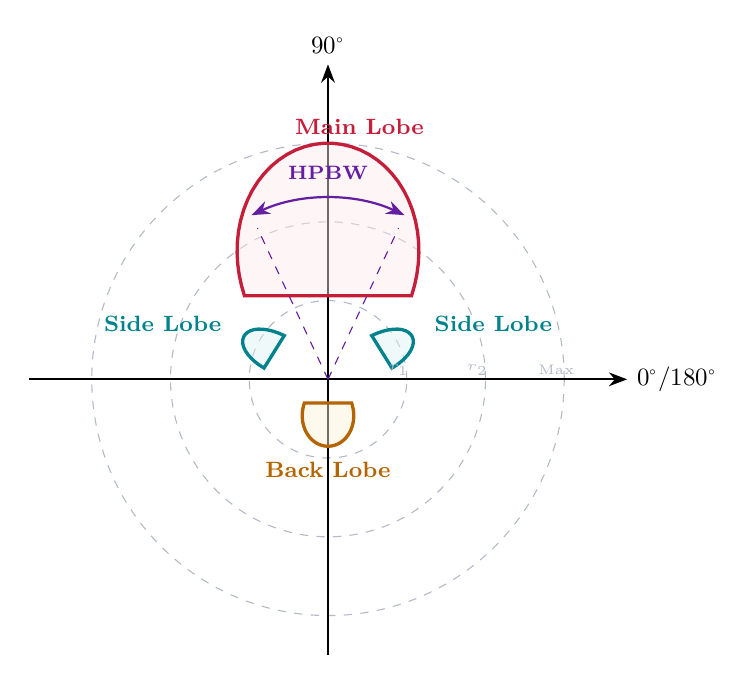
\begin{tikzpicture}[scale=1.0]
  % ── Polar grid ──────────────────────────────────────────────────────────────
  \draw[dashed, color=mgframe, thin] (0,0) circle (1);
  \draw[dashed, color=mgframe, thin] (0,0) circle (2);
  \draw[dashed, color=mgframe, thin] (0,0) circle (3);
  % Axes
  \draw[-Stealth, thick] (-3.8,0) -- (3.8,0) node[right, font=\small] {$0^\circ / 180^\circ$};
  \draw[-Stealth, thick] (0,-3.5) -- (0,4.0) node[above, font=\small] {$90^\circ$};

  % ── Main Lobe (pointing up, $r = 3\cos^2\theta'$, $\theta' = t-90$) ─────────
  \draw[very thick, color=myred, fill=hdrred, fill opacity=0.45, domain=45:135, samples=40, variable=\t]
    plot ({3*cos(\t-90)*cos(\t-90)*cos(\t)}, {3*cos(\t-90)*cos(\t-90)*sin(\t)}) -- cycle;

  % ── Side Lobes ────────────────────────────────────────────────────────────
  % Right side lobe
  \draw[very thick, color=myteal, fill=hdrteal, fill opacity=0.45, domain=10:45, samples=20, variable=\t]
    plot ({1.2*cos(2*(\t-27))*cos(2*(\t-27))*cos(\t)}, {1.2*cos(2*(\t-27))*cos(2*(\t-27))*sin(\t)}) -- cycle;
  % Left side lobe
  \draw[very thick, color=myteal, fill=hdrteal, fill opacity=0.45, domain=135:170, samples=20, variable=\t]
    plot ({1.2*cos(2*(\t-153))*cos(2*(\t-153))*cos(\t)}, {1.2*cos(2*(\t-153))*cos(2*(\t-153))*sin(\t)}) -- cycle;

  % ── Back Lobe ─────────────────────────────────────────────────────────────
  \draw[very thick, color=myamber, fill=hdramber, fill opacity=0.45, domain=225:315, samples=40, variable=\t]
    plot ({0.85*cos(\t-270)*cos(\t-270)*cos(\t)}, {0.85*cos(\t-270)*cos(\t-270)*sin(\t)}) -- cycle;

  % ── HPBW annotation ────────────────────────────────────────────────────────
  \draw[dashed, thin, color=mypurple] (0,0) -- ({2.12*cos(115)},{2.12*sin(115)});
  \draw[dashed, thin, color=mypurple] (0,0) -- ({2.12*cos(65)},{2.12*sin(65)});
  \draw[Stealth-Stealth, thick, color=mypurple]
    ({2.3*cos(115)},{2.3*sin(115)}) arc (115:65:2.3)
    node[midway, above=3pt, font=\scriptsize\bfseries\color{mypurple}] {HPBW};

  % ── Labels ──────────────────────────────────────────────────────────────────
  \node[font=\footnotesize\bfseries\color{myred}] at (0.4, 3.2) {Main Lobe};
  \node[font=\footnotesize\bfseries\color{myteal}] at (2.1, 0.7) {Side Lobe};
  \node[font=\footnotesize\bfseries\color{myteal}] at (-2.1, 0.7) {Side Lobe};
  \node[font=\footnotesize\bfseries\color{myamber}] at (0, -1.15) {Back Lobe};
  % Scale labels
  \node[font=\tiny\color{mgframe}] at (0.9, 0.12) {$r_1$};
  \node[font=\tiny\color{mgframe}] at (1.9, 0.12) {$r_2$};
  \node[font=\tiny\color{mgframe}] at (2.9, 0.12) {Max};
\end{tikzpicture}
\end{tcolorbox}

\subsection{Half-Power Beamwidth (HPBW) and First-Null Beamwidth (FNBW)}
\begin{itemize}[leftmargin=*, itemsep=3pt]
  \item \textbf{Half-Power Beamwidth (HPBW):} The angular width of the main beam between two directions where the radiation intensity is half ($3\,\text{dB}$ below) the maximum value.
  \item \textbf{First-Null Beamwidth (FNBW):} The angular width between the first two nulls (where the radiation intensity drops to zero) on either side of the main beam.
\end{itemize}

\subsection{Antenna Field Regions}
The space surrounding an antenna is divided into three regions depending on the distance $r$ from the antenna. Let $D$ be the maximum dimension of the antenna, and $\lambda$ be the wavelength.

\begin{tcolorbox}[tikzbox, title={Antenna Field Regions}]
\centering
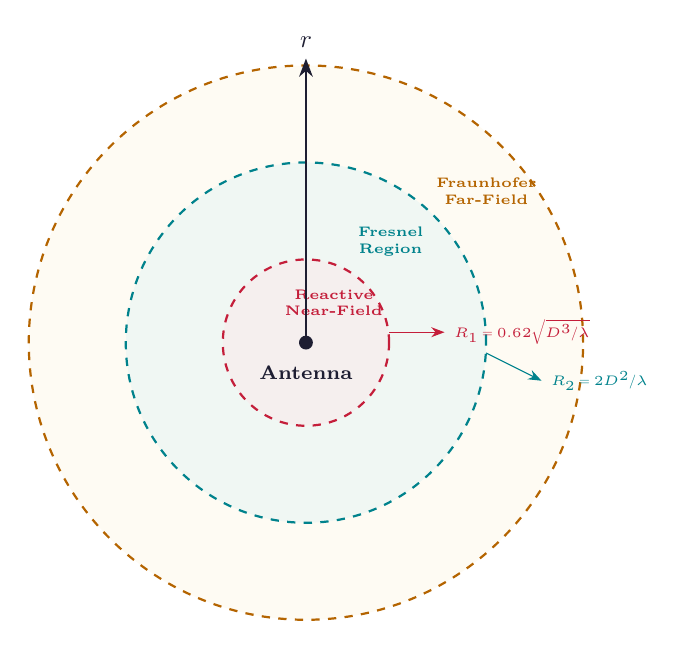
\begin{tikzpicture}[scale=0.88]
  \coordinate (O) at (0,0);

  % Fill regions from outside in (painter's algorithm)
  \fill[hdramber, fill opacity=0.3] (O) circle (4.0);
  \fill[hdrteal, fill opacity=0.4] (O) circle (2.6);
  \fill[hdrred, fill opacity=0.5] (O) circle (1.2);

  % Dashed boundary circles
  \draw[thick, color=myred, dashed] (O) circle (1.2);
  \draw[thick, color=myteal, dashed] (O) circle (2.6);
  \draw[thick, color=myamber, dashed] (O) circle (4.0);

  % Antenna at center
  \fill[mydark] (O) circle (0.1);
  \node[below=5pt, font=\scriptsize\bfseries\color{mydark}] at (O) {Antenna};

  % Region name labels (inside each band)
  \node[align=center, font=\tiny\bfseries\color{myred}] at (55:0.7) {Reactive\\Near-Field};
  \node[align=center, font=\tiny\bfseries\color{myteal}] at (50:1.9) {Fresnel\\Region};
  \node[align=center, font=\tiny\bfseries\color{myamber}] at (40:3.4) {Fraunhofer\\Far-Field};

  % Boundary annotation arrows on horizontal axis
  \draw[thin, -Stealth, color=myred] (1.2, 0.15) -- (2.0, 0.15);
  \node[right, font=\tiny\color{myred}] at (2.0, 0.15) {$R_1 = 0.62\sqrt{D^3/\lambda}$};

  \draw[thin, -Stealth, color=myteal] (2.6, -0.15) -- (3.4, -0.55);
  \node[right, font=\tiny\color{myteal}] at (3.4, -0.55) {$R_2 = 2D^2/\lambda$};

  % Radial axis
  \draw[-Stealth, thick, color=mydark] (0,0) -- (0, 4.1) node[above, font=\small] {$r$};
\end{tikzpicture}
\end{tcolorbox}

\begin{enumerate}[label=\textbf{\arabic*.}, leftmargin=*, itemsep=4pt]
  \item \textbf{Reactive Near-Field Region:} The region immediately surrounding the antenna where the reactive fields (non-radiating, storing energy like a capacitor or inductor) are dominant. The boundary is:
  \[
  r < R_1 = 0.62\sqrt{\frac{D^3}{\lambda}}
  \]
  \item \textbf{Radiating Near-Field (Fresnel) Region:} The region between the reactive near-field and far-field where radiation fields dominate, but the angular field distribution depends on the distance from the antenna (because phase variations across the aperture are significant). The boundary is:
  \[
  0.62\sqrt{\frac{D^3}{\lambda}} \le r < R_2 = \frac{2D^2}{\lambda}
  \]
  \item \textbf{Far-Field (Fraunhofer) Region:} The region where the angular distribution of the electromagnetic fields is independent of the distance. The wave behaves as a local transverse electromagnetic (TEM) plane wave, where the electric and magnetic fields are orthogonal to the direction of propagation. The boundary is:
  \[
  r \ge \frac{2D^2}{\lambda} \quad (\text{provided } D \gg \lambda \text{ and } r \gg \lambda)
  \]
\end{enumerate}

% ===============================================================================
\section{Reciprocity, Directivity, and Gain}
% ===============================================================================

\subsection{Reciprocity Theorem}
The reciprocity theorem states that the electrical characteristics (such as radiation pattern, directivity, input impedance, and effective length) of an antenna remain identical whether it is operated as a transmitter or a receiver.

\textbf{Mathematical Formulation:} Let two antennas $A$ and $B$ exist in a linear, isotropic, and homogenous medium. If a voltage source $V_1$ applied at the terminals of antenna $A$ produces a current $I_2$ at the short-circuited terminals of antenna $B$, and a voltage source $V_2$ applied at the terminals of antenna $B$ produces a current $I_1$ at the short-circuited terminals of antenna $A$, then:
\[
\text{If } V_1 = V_2 \implies I_1 = I_2 \quad (\text{or } Z_{12} = Z_{21})
\]

\subsection{Directivity and Gain}
\begin{itemize}[leftmargin=*, itemsep=3pt]
  \item \textbf{Radiation Intensity ($U$):} The power radiated per unit solid angle (expressed in Watts/steradian).
  \[
  U(\theta, \phi) = r^2 W_{rad}(\theta, \phi)
  \]
  where $W_{rad}$ is the radial component of the Poynting vector.
  \item \textbf{Directivity ($D$):} The ratio of the radiation intensity in a given direction to the average radiation intensity (which is equal to the intensity of an isotropic radiator).
  \[
  D = \frac{U(\theta, \phi)}{U_0} = \frac{4\pi U(\theta, \phi)}{P_{rad}}
  \]
  where $P_{rad} = \int_{0}^{2\pi}\int_{0}^{\pi} U(\theta, \phi) \sin\theta \, d\theta \, d\phi$ is the total radiated power.
  \item \textbf{Gain ($G$):} The ratio of the radiation intensity in a given direction to the radiation intensity that would be obtained if the total power accepted by the antenna ($P_{in}$) was radiated isotropically.
  \[
  G = \frac{4\pi U(\theta, \phi)}{P_{in}}
  \]
  \item \textbf{Relationship between Gain and Directivity:}
  \[
  G = \eta_{cd} D
  \]
  where $\eta_{cd}$ is the antenna radiation efficiency ($0 \le \eta_{cd} \le 1$), representing conduction and dielectric losses.
  \item \textbf{Narrow-Beam Directivity Approximation:} For antennas with a well-defined beam in both principal planes, directivity can be estimated directly from the half-power beamwidths (in degrees):
  \[
  D \approx \frac{41253}{\Theta_{E} \cdot \Theta_{H}}
  \]
  where $\Theta_E$ and $\Theta_H$ are the HPBW in the E-plane and H-plane respectively (in degrees). This formula is accurate to within $\pm 1\,\text{dB}$ for most practical antennas.\end{itemize}

% ===============================================================================
\section{Effective Aperture and Polarization}
% ===============================================================================

\subsection{Effective Aperture (\texorpdfstring{$A_e$}{Ae})}
The \textbf{effective aperture} (or effective area) of a receiving antenna is a measure of its ability to extract power from a passing electromagnetic wave. It is defined as the ratio of the delivered power $P_L$ at the load terminals (matched condition) to the power density $W_{inc}$ of the incident wave.

\begin{tcolorbox}[formulabox, title={\textbf{Effective Aperture and Directivity Relation}}]
The delivered power is $P_L = A_e W_{inc}$. The relationship between the maximum effective aperture $A_{em}$ and the maximum directivity $D_0$ for any antenna is:
\[
A_{em} = \frac{\lambda^2}{4\pi} D_0
\]
\end{tcolorbox}

\subsection{Polarization}
The \textbf{polarization} of an antenna is defined as the polarization of the electromagnetic wave radiated by the antenna in a given direction. It describes the orientation of the electric field vector $\vec{E}$ as a function of time.

There are three main types of polarization:
\begin{itemize}[leftmargin=*, itemsep=3pt]
  \item \textbf{Linear Polarization:} The electric field vector oscillates along a straight line. This occurs when the two orthogonal field components $E_x$ and $E_y$ are in-phase (phase difference $\Delta \psi = 0$ or $180^\circ$).
  \item \textbf{Circular Polarization:} The electric field vector traces out a circle. This requires $E_x = E_y$ and $\Delta \psi = \pm 90^\circ$ ($\pm \pi/2$ rad).
  \item \textbf{Elliptical Polarization:} The electric field vector traces an ellipse. This is the general case when $E_x \neq E_y$ and/or the phase difference is arbitrary (excluding linear/circular conditions).
\end{itemize}

\begin{tcolorbox}[tikzbox, title={Traces of Polarization States}]
\centering
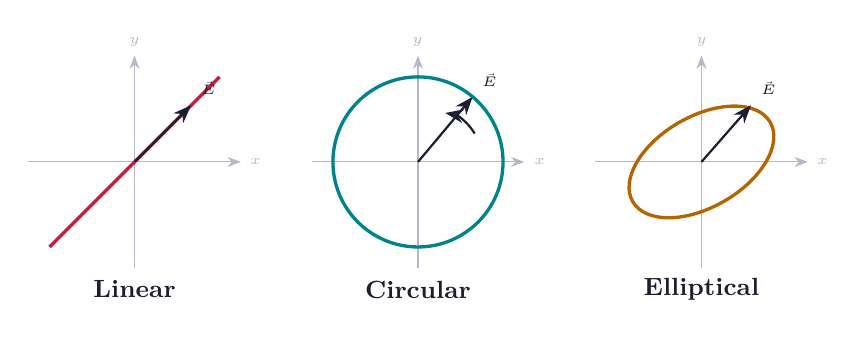
\begin{tikzpicture}[scale=0.9]
  % Linear Polarization
  \begin{scope}[xshift=-4cm]
    \draw[-Stealth, color=mgframe] (-1.5,0) -- (1.5,0) node[right, font=\tiny] {$x$};
    \draw[-Stealth, color=mgframe] (0,-1.5) -- (0,1.5) node[above, font=\tiny] {$y$};
    \draw[very thick, color=myred] (-1.2,-1.2) -- (1.2,1.2);
    \draw[-Stealth, thick, color=mydark] (0,0) -- (0.8,0.8) node[above right, font=\tiny] {$\vec{E}$};
    \node[font=\small\bfseries\color{mydark}] at (0,-1.8) {Linear};
  \end{scope}

  % Circular Polarization
  \begin{scope}[xshift=0cm]
    \draw[-Stealth, color=mgframe] (-1.5,0) -- (1.5,0) node[right, font=\tiny] {$x$};
    \draw[-Stealth, color=mgframe] (0,-1.5) -- (0,1.5) node[above, font=\tiny] {$y$};
    \draw[very thick, color=myteal] (0,0) circle (1.2);
    \draw[-Stealth, thick, color=mydark] (0,0) -- ({1.2*cos(50)}, {1.2*sin(50)}) node[above right, font=\tiny] {$\vec{E}$};
    \draw[-Stealth, thick, color=mydark] (0.8, 0.4) arc (30:80:0.6);
    \node[font=\small\bfseries\color{mydark}] at (0,-1.8) {Circular};
  \end{scope}

  % Elliptical Polarization
  \begin{scope}[xshift=4cm]
    \draw[-Stealth, color=mgframe] (-1.5,0) -- (1.5,0) node[right, font=\tiny] {$x$};
    \draw[-Stealth, color=mgframe] (0,-1.5) -- (0,1.5) node[above, font=\tiny] {$y$};
    \draw[very thick, color=myamber, rotate=30, xscale=1.4, yscale=0.8] (0,0) circle (0.8);
    \draw[-Stealth, thick, color=mydark] (0,0) -- (0.7,0.8) node[above right, font=\tiny] {$\vec{E}$};
    \node[font=\small\bfseries\color{mydark}] at (0,-1.8) {Elliptical};
  \end{scope}
\end{tikzpicture}
\end{tcolorbox}

% ===============================================================================
\section{Input Impedance, Efficiency, and Friis Transmission Equation}
% ===============================================================================

\subsection{Input Impedance}
The \textbf{input impedance} ($Z_{in}$) of an antenna is the impedance presented by the antenna at its terminals. It consists of a real part (input resistance $R_{in}$) and an imaginary part (input reactance $X_{in}$):
\[
Z_{in} = R_{in} + j X_{in}
\]
The input resistance $R_{in}$ is composed of:
\[
R_{in} = R_r + R_L
\]
where $R_r$ is the \textbf{radiation resistance} (representing the power converted into radiated waves) and $R_L$ is the \textbf{loss resistance} (representing conduction and dielectric heating losses).

\subsection{Antenna Efficiency}
The total antenna efficiency ($\eta_0$) accounts for all losses in the system:
\[
\eta_0 = \eta_r \eta_c \eta_d = \eta_r \eta_{cd}
\]
where:
\begin{itemize}[leftmargin=*, itemsep=1pt]
  \item $\eta_r = 1 - |\Gamma|^2$ is the reflection (mismatch) efficiency ($\Gamma$ is the reflection coefficient).
  \item $\eta_c$ is the conduction efficiency.
  \item $\eta_d$ is the dielectric efficiency.
  \item $\eta_{cd} = \eta_c \eta_d = \frac{R_r}{R_r + R_L}$ is the radiation efficiency.
\end{itemize}

\subsection{Friis Transmission Equation}
The Friis transmission equation relates the power received by an antenna ($P_r$) to the power transmitted by another antenna ($P_t$), separated by a distance $r$ in free space.

\begin{tcolorbox}[formulabox, title={\textbf{Friis Transmission Formula}}]
Let $G_t$ be the gain of the transmitting antenna and $G_r$ be the gain of the receiving antenna. The received power is:
\[
P_r = P_t G_t G_r \left( \frac{\lambda}{4\pi r} \right)^{\!2} (PLF)
\]
where $PLF = |\hat{\rho}_t \cdot \hat{\rho}_r|^2$ is the Polarization Loss Factor ($0 \le PLF \le 1$). For matched polarizations, $PLF = 1$.
\end{tcolorbox}

\textbf{Derivation:}
\begin{enumerate}[label=\textbf{\arabic*.}, leftmargin=*, itemsep=3pt]
  \item The power density $W_t$ radiated by an isotropic source at distance $r$ is:
  \[
  W_{isotropic} = \frac{P_t}{4\pi r^2}
  \]
  \item For a directive transmitting antenna with gain $G_t$, the power density in its direction of maximum radiation is:
  \[
  W_t = \frac{P_t G_t}{4\pi r^2}
  \]
  \item The receiving antenna collects this energy using its effective aperture $A_{er}$:
  \[
  P_r = W_t A_{er} = \left( \frac{P_t G_t}{4\pi r^2} \right) A_{er}
  \]
  \item Using the relationship between effective aperture and gain ($A_{er} = G_r \frac{\lambda^2}{4\pi}$):
  \[
  P_r = \left( \frac{P_t G_t}{4\pi r^2} \right) \left( G_r \frac{\lambda^2}{4\pi} \right) = P_t G_t G_r \left( \frac{\lambda}{4\pi r} \right)^{\!2}
  \]
\end{enumerate}

% ===============================================================================
\section{Radiation Integrals and Potential Functions}
% ===============================================================================

To calculate the fields radiated by an antenna, we use auxiliary potential functions rather than solving Maxwell's equations directly. The most common vector potentials are:
\begin{itemize}[leftmargin=*, itemsep=3pt]
  \item $\vec{A}$ (Magnetic Vector Potential): Created by electric current sources $\vec{J}$.
  \item $\vec{F}$ (Electric Vector Potential): Created by magnetic current sources $\vec{M}$ (equivalent currents).
\end{itemize}

\subsection{Relationship between Potentials and Fields}
For a magnetic vector potential $\vec{A}$, the magnetic flux density is:
\[
\vec{B} = \nabla \times \vec{A} \implies \vec{H} = \frac{1}{\mu} \nabla \times \vec{A}
\]
From Maxwell's equation $\nabla \times \vec{E} = -j\omega\mu\vec{H}$, we substitute $\vec{H}$ to get:
\[
\vec{E} = -j\omega\vec{A} - \frac{j}{\omega\mu\epsilon}\nabla(\nabla \cdot \vec{A})
\]

\subsection{Inhomogeneous Helmholtz Wave Equation}
From Maxwell's equations, the potential function $\vec{A}$ satisfies:
\[
\nabla^2 \vec{A} + k^2 \vec{A} = -\mu \vec{J}
\]
where $k = \omega\sqrt{\mu\epsilon} = 2\pi/\lambda$ is the wave number. 

The solution to this inhomogeneous wave equation in free space is:
\[
\vec{A}(x, y, z) = \frac{\mu}{4\pi} \iiint_{V} \vec{J}(x', y', z') \frac{e^{-j k R}}{R} \, dV'
\]
where:
\begin{itemize}[leftmargin=*, itemsep=1pt]
  \item $(x', y', z')$ are the coordinates of the source currents.
  \item $(x, y, z)$ are the coordinates of the observation point.
  \item $R = \sqrt{(x-x')^2 + (y-y')^2 + (z-z')^2}$ is the distance from the source point to the observation point.
\end{itemize}

In the far field, the distance $R$ can be approximated as $R \approx r - r'\cos\psi$ for phase terms, and $R \approx r$ for amplitude terms. This simplifies the vector potential to:
\[
\vec{A} \approx \frac{\mu e^{-jkr}}{4\pi r} \iiint_{V} \vec{J}(x', y', z') e^{jkr'\cos\psi} \, dV'
\]

% ===============================================================================
% MANDATORY QUICK REVISION PAGE
% ===============================================================================
\newpage
\begin{center}
  {\large\bfseries\color{myred} Quick Revision --- Module 1}\\[3pt]
  {\small\color{mydark} Fundamental Concepts of Antennas $|$ PE-EC801A}
\end{center}
\noindent{\color{myred}\rule{\linewidth}{1.2pt}}
\vspace{4pt}

\begin{tcolorbox}[formulabox, title={\textbf{Key Formulas and Metrics at a Glance}}]
\renewcommand{\arraystretch}{1.35}
\begin{tabularx}{\linewidth}{B{5.0cm} X}
Radiation Intensity ($U$) & $U = r^2 W_{rad}$ \quad (Watts/steradian) \\[4pt]
Directivity ($D$) & $D = \frac{4\pi U}{P_{rad}}$ \\[4pt]
Gain ($G$) & $G = \eta_{cd} D = \frac{4\pi U}{P_{in}}$ \\[4pt]
Effective Aperture-Gain Relation & $A_{em} = \frac{\lambda^2}{4\pi} D_0$ \\[4pt]
Narrow-Beam Directivity Approx. & $D \approx \frac{41253}{\Theta_E \cdot \Theta_H}$ \quad ($\Theta$ in degrees) \\[4pt]
Friis Transmission Equation & $P_r = P_t G_t G_r \left( \frac{\lambda}{4\pi r} \right)^{\!2} (PLF)$ \\[4pt]
Helmholtz Equation Solution & $\vec{A} = \frac{\mu}{4\pi} \iiint \vec{J} \frac{e^{-jkR}}{R} dV'$ \\[4pt]
Helmholtz Wave Number ($k$) & $k = \frac{2\pi}{\lambda} = \omega\sqrt{\mu\epsilon}$ \\[4pt]
\end{tabularx}
\end{tcolorbox}

\begin{tcolorbox}[defbox, title={\textbf{One-Line Definitions}}]
\begin{itemize}[leftmargin=*, itemsep=2pt, topsep=0pt]
  \item \textbf{Transducer:} A device that converts energy from one form to another; antennas convert guided electromagnetic waves into free-space waves.
  \item \textbf{Radiation Pattern:} The spatial distribution of physical quantities (like power or field intensity) radiated by an antenna.
  \item \textbf{HPBW:} The angle between the two directions in which the radiation intensity is half of the maximum.
  \item \textbf{Reactive Near-Field:} The region closest to the antenna where reactive non-radiating energy is stored.
  \item \textbf{Far-Field (Fraunhofer) Region:} The region where waves behave as transverse electromagnetic (TEM) plane waves and the pattern does not change with distance.
  \item \textbf{Reciprocity:} The property where transmitting and receiving characteristics of an antenna are identical.
  \item \textbf{Polarization Loss Factor (PLF):} A factor measuring mismatch loss between the polarization of a wave and the receiving antenna.
\end{itemize}
\end{tcolorbox}

\begin{tcolorbox}[exambox, title={\textbf{Frequently Asked / Viva Questions}}]
\begin{enumerate}[topsep=0pt, label=\textbf{Q\arabic*.}, itemsep=5pt]
  \item \Q{What is the physical mechanism of antenna radiation?}
    Radiation is produced by accelerated or decelerated charges, or equivalently, by time-varying currents. Charges oscillating on a conductor generate changing electric and magnetic fields that propagate outward as electromagnetic waves.
  \item \Q{State the three field regions of an antenna and write their boundary equations.}
    \begin{itemize}[leftmargin=*, itemsep=1pt, topsep=2pt]
      \item Reactive near-field: $r < 0.62\sqrt{D^3/\lambda}$
      \item Radiating near-field (Fresnel): $0.62\sqrt{D^3/\lambda} \le r < 2D^2/\lambda$
      \item Far-field (Fraunhofer): $r \ge 2D^2/\lambda$
    \end{itemize}
  \item \Q{Define directivity. How is it different from power gain?}
    Directivity is the ratio of radiation intensity in a given direction to average radiation intensity (purely directional focus). Power gain also accounts for efficiency (conduction and dielectric losses) in addition to directional focus ($G = \eta_{cd} D$).
  \item \Q{State the reciprocity theorem for antennas.}
    The transmitting and receiving properties of an antenna (pattern, impedance, directivity) are identical. A voltage source $V$ at the terminals of antenna $A$ produces current $I$ at antenna $B$, and the same source $V$ at $B$ produces the same current $I$ at $A$.
  \item \Q{What is Polarization Loss Factor (PLF)? What is its value for a vertically polarized antenna receiving a horizontally polarized wave?}
    PLF measures the loss due to polarization mismatch between the incoming wave and the receiving antenna. For orthogonal polarizations (vertical vs. horizontal), $PLF = 0$ (zero power is received).
  \item \Q{Derive the relationship between effective aperture and directivity.}
    Under thermodynamic equilibrium, the ratio of maximum effective aperture to directivity is constant for all antennas: $\frac{A_{em}}{D_0} = \frac{\lambda^2}{4\pi}$. Thus, $A_{em} = \frac{\lambda^2}{4\pi} D_0$.
  \item \Q{Explain the physical meaning of radiation resistance.}
    It is an equivalent resistance that would dissipate the same amount of power as heat as the antenna actually radiates into free space: $R_r = \frac{2 P_{rad}}{I_0^2}$.
  \item \Q{State the Friis transmission equation. What parameters does it relate?}
    $P_r = P_t G_t G_r \left( \frac{\lambda}{4\pi r} \right)^2$. It relates received power ($P_r$) to transmitted power ($P_t$) based on antenna gains ($G_t, G_r$), operating wavelength ($\lambda$), and separation distance ($r$).
  \item \Q{What are auxiliary potential functions? Why are they used?}
    Auxiliary vector potentials ($\vec{A}$ and $\vec{F}$) are mathematical helper functions. They are used because it is much simpler to compute the potentials from the current distributions ($\vec{J}, \vec{M}$) and then take derivatives to get the fields ($\vec{E}, \vec{H}$), rather than solving Maxwell's equations directly.
  \item \Q{Under what conditions does a charge radiate?}
    A charge radiates only if it is accelerated or decelerated. A stationary charge or a charge moving with constant velocity along a straight, infinite transmission line does not radiate.
  \end{enumerate}
\end{tcolorbox}

\begin{tcolorbox}[tikzbox, title={Comparison of Field Regions}]
\centering
\renewcommand{\arraystretch}{1.55}
{\renewcommand{\arraystretch}{1.55}%
\begin{tabularx}{\linewidth}{|B{3.2cm}|Y|Y|Y|}
\hline
\multicolumn{1}{|>{\centering\arraybackslash}m{3.2cm}|}{\textbf{Property}} &
\multicolumn{1}{>{\centering\arraybackslash}Y|}{\textbf{Reactive Near-Field}} &
\multicolumn{1}{>{\centering\arraybackslash}Y|}{\textbf{Radiating Near-Field}} &
\multicolumn{1}{>{\centering\arraybackslash}Y|}{\textbf{Far-Field}} \\
\hline
Dominant Field Type & Reactive fields (energy storage) & Radiating fields (reactive fields decay) & Radiating fields (pure real power) \\
\hline
Pattern Shape & Changes drastically with distance & Varies with distance ($r$) & Independent of distance ($r$) \\
\hline
Phase Fronts & Highly complex & Non-spherical & Spherical (locally planar) \\
\hline
Wave Impedance & Complex (reactive) & Varies & Real ($\approx 377\,\Omega$ in free space) \\
\hline
\end{tabularx}}
\end{tcolorbox}


% -- Module 2 -----------------------------------------------------------------
\modulestart{2}{Infinitesimal Dipole}

\section{Infinitesimal Dipole}
% ===============================================================================

\begin{tcolorbox}[defbox, title={\textbf{Definition of Infinitesimal Dipole}}]
An \textbf{infinitesimal dipole} (also known as a Hertzian dipole) is a thin linear antenna whose length $dl$ is extremely small compared to the wavelength ($dl \ll \lambda$) and whose current is assumed to be uniform ($I(z) = I_0 = \text{constant}$) over its entire length.
\end{tcolorbox}

\subsection{Coordinate System and Potential Derivation}
Consider a wire of length $dl$ placed symmetrically at the origin along the $z$-axis. Since the current is along $z$, the current density is $\vec{J} = \hat{a}_z I_0 \delta(x')\delta(y')$ for $-dl/2 \le z' \le dl/2$. 

\begin{tcolorbox}[tikzbox, title={Infinitesimal Dipole Geometry}]
\centering
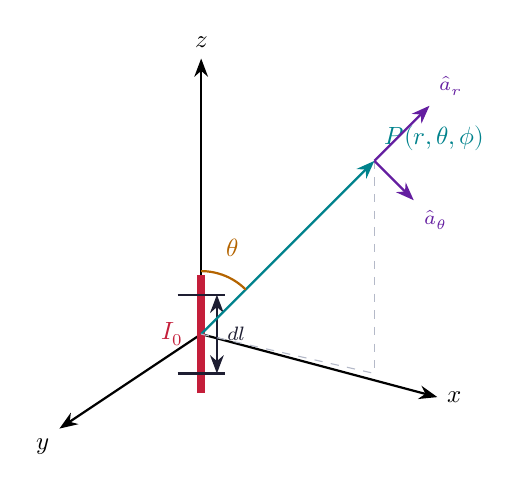
\begin{tikzpicture}[scale=1.0]
  % Spherical coordinates axes
  \draw[-Stealth, thick] (0,0) -- (0,3.5) node[above, font=\small] {$z$};
  \draw[-Stealth, thick] (0,0) -- (3.0,-0.8) node[right, font=\small] {$x$};
  \draw[-Stealth, thick] (0,0) -- (-1.8,-1.2) node[below left, font=\small] {$y$};

  % Dipole wire
  \draw[line width=3pt, color=myred] (0,-0.75) -- (0,0.75);
  \draw[thick, color=mydark] (-0.3, 0.5) -- (0.3, 0.5);
  \draw[thick, color=mydark] (-0.3, -0.5) -- (0.3, -0.5);
  \draw[Stealth-Stealth, thick, color=mydark] (0.2, -0.5) -- (0.2, 0.5) node[midway, right, font=\scriptsize] {$dl$};
  \node[left=3pt, font=\small\bfseries\color{myred}] at (0,0) {$I_0$};

  % Vector to observation point
  \draw[-Stealth, thick, color=myteal] (0,0) -- (2.2,2.2) node[above right, font=\small] {$P(r, \theta, \phi)$};
  \draw[dashed, color=mgframe] (2.2,2.2) -- (2.2,-0.5);
  \draw[dashed, color=mgframe] (0,0) -- (2.2,-0.5);

  % Angles
  \draw[thick, color=myamber] (0,0.8) arc (90:45:0.8);
  \node[color=myamber, font=\small\bfseries] at (0.4, 1.1) {$\theta$};

  % Unit vectors
  \draw[-Stealth, thick, color=mypurple] (2.2,2.2) -- (2.9,2.9) node[above right, font=\scriptsize] {$\hat{a}_r$};
  \draw[-Stealth, thick, color=mypurple] (2.2,2.2) -- (2.7,1.7) node[below right, font=\scriptsize] {$\hat{a}_\theta$};

\end{tikzpicture}
\end{tcolorbox}

The magnetic vector potential $\vec{A}$ at a distance $r$ (since $r \gg dl$) is:
\[
\vec{A}(r) = \hat{a}_z \frac{\mu I_0 dl}{4\pi r} e^{-jkr}
\]
Using coordinate transformations, the spherical components of $\vec{A}$ are:
\[
A_r = A_z \cos\theta = \frac{\mu I_0 dl \cos\theta}{4\pi r} e^{-jkr}
\]
\[
A_\theta = -A_z \sin\theta = -\frac{\mu I_0 dl \sin\theta}{4\pi r} e^{-jkr}
\]
\[
A_\phi = 0
\]

\subsection{Electromagnetic Field Equations}
By applying Maxwell's relations ($\vec{H} = \frac{1}{\mu} \nabla \times \vec{A}$ and $\vec{E} = \frac{1}{j\omega\epsilon} \nabla \times \vec{H}$), we obtain the complete field equations:
\[
H_\phi = j \frac{k I_0 dl \sin\theta}{4\pi r} \left[ 1 + \frac{1}{jkr} \right] e^{-jkr}
\]
\[
E_r = \frac{2 I_0 dl \eta \cos\theta}{4\pi r^2} \left[ 1 + \frac{1}{jkr} \right] e^{-jkr}
\]
\[
E_\theta = j \frac{k I_0 dl \eta \sin\theta}{4\pi r} \left[ 1 + \frac{1}{jkr} - \frac{1}{(kr)^2} \right] e^{-jkr}
\]
where $\eta = \sqrt{\mu/\epsilon} \approx 120\pi \approx 377\,\Omega$ is the intrinsic impedance of free space. Other components $H_r = H_\theta = E_\phi = 0$.

\subsection{Far-Field Approximation and Radiation Resistance}
For the far field ($kr \gg 1$), terms containing $1/(kr)^2$ and $1/(kr)^3$ can be neglected. The fields simplify to:
\[
H_\phi \approx j \frac{I_0 k dl \sin\theta}{4\pi r} e^{-jkr}
\]
\[
E_\theta \approx j \eta \frac{I_0 k dl \sin\theta}{4\pi r} e^{-jkr}
\]
The total power radiated is found by integrating the Poynting vector over a closed sphere:
\[
P_{rad} = \int_{0}^{2\pi}\int_{0}^{\pi} \frac{1}{2} \text{Re}(E_\theta H_\phi^*) r^2 \sin\theta \, d\theta \, d\phi = 40 \pi^2 I_0^2 \left(\frac{dl}{\lambda}\right)^{\!2}
\]
Since $P_{rad} = \frac{1}{2} I_0^2 R_r$, the radiation resistance $R_r$ of an infinitesimal dipole is:
\[
R_r = 80 \pi^2 \left(\frac{dl}{\lambda}\right)^{\!2}
\]

\begin{tcolorbox}[defbox, title={\textbf{Note: The Short Dipole}}]
For a \textbf{short dipole} (length $l \ll \lambda$, but current decreases linearly from $I_0$ at the center to $0$ at the ends), the average current is $I_0/2$. The radiation resistance is $1/4$ of the infinitesimal dipole:
\[
R_r = 20\pi^2 \left(\frac{l}{\lambda}\right)^{\!2}
\]
\end{tcolorbox}

% ===============================================================================
\section{Finite-Length Dipole}
% ===============================================================================

When the antenna length is comparable to the wavelength, the current is no longer uniform. It forms a standing wave with a sinusoidal distribution (assuming thin wire and zero current at the ends).

\subsection{Current Distribution}
For a dipole of length $l$ placed along the $z$-axis, the current distribution is:
\[
I(z') = I_0 \sin\left[ k \left( \frac{l}{2} - |z'| \right) \right], \quad -l/2 \le z' \le l/2
\]

\begin{tcolorbox}[tikzbox, title={Current Distributions on Dipoles}]
\centering
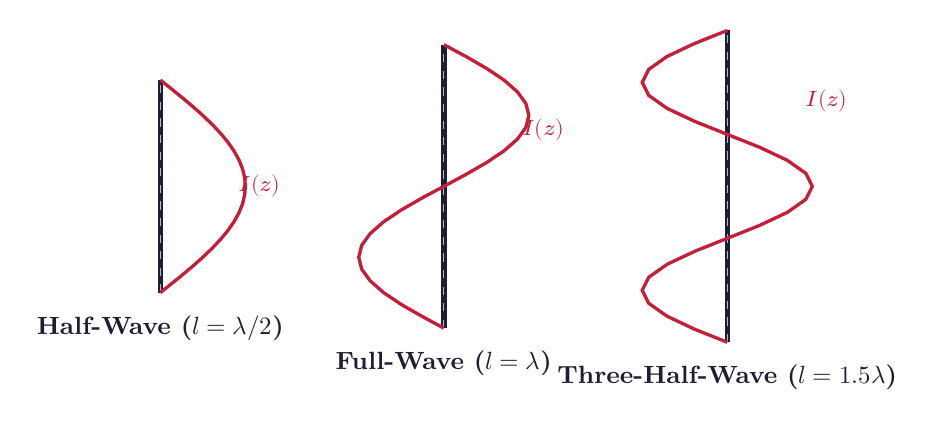
\begin{tikzpicture}[scale=0.9]
  % 1/2 Wave Dipole
  \begin{scope}[xshift=-4cm]
    \draw[line width=2pt, color=mydark] (0,-1.5) -- (0,1.5);
    \draw[dashed, color=mgframe] (0,-1.5) -- (0,1.5);
    % Current curve
    \draw[very thick, color=myred, domain=-1.5:1.5] plot ({1.2*cos(90*\x/1.5)}, \x);
    \node[font=\footnotesize\bfseries\color{myred}] at (1.4,0) {$I(z)$};
    \node[font=\small\bfseries\color{mydark}] at (0,-2.0) {Half-Wave ($l = \lambda/2$)};
  \end{scope}

  % Full Wave Dipole
  \begin{scope}[xshift=0cm]
    \draw[line width=2pt, color=mydark] (0,-2.0) -- (0,2.0);
    \draw[dashed, color=mgframe] (0,-2.0) -- (0,2.0);
    % Current curve
    \draw[very thick, color=myred, domain=-2:2] plot ({1.2*sin(180*\x/2.0)}, \x);
    \node[font=\footnotesize\bfseries\color{myred}] at (1.4,0.8) {$I(z)$};
    \node[font=\small\bfseries\color{mydark}] at (0,-2.5) {Full-Wave ($l = \lambda$)};
  \end{scope}

  % 3/2 Wave Dipole
  \begin{scope}[xshift=4cm]
    \draw[line width=2pt, color=mydark] (0,-2.2) -- (0,2.2);
    \draw[dashed, color=mgframe] (0,-2.2) -- (0,2.2);
    % Current curve
    \draw[very thick, color=myred, domain=-2.2:2.2] plot ({1.2*cos(270*\x/2.2)}, \x);
    \node[font=\footnotesize\bfseries\color{myred}] at (1.4,1.2) {$I(z)$};
    \node[font=\small\bfseries\color{mydark}] at (0,-2.7) {Three-Half-Wave ($l = 1.5\lambda$)};
  \end{scope}
\end{tikzpicture}
\end{tcolorbox}

\subsection{Far-Field Radiation Pattern}
By treating the finite dipole as an infinite sum of infinitesimal dipoles and integrating the contributions, the far-field electric field is:
\[
E_\theta \approx j \eta \frac{I_0 e^{-jkr}}{2\pi r} \left[ \frac{\cos\left(\frac{kl}{2}\cos\theta\right) - \cos\left(\frac{kl}{2}\right)}{\sin\theta} \right]
\]
\[
H_\phi = \frac{E_\theta}{\eta}
\]

\subsection{The Half-Wave Dipole (\texorpdfstring{$l = \lambda/2$}{l = lambda/2})}
Setting $l = \lambda/2$ (and thus $kl/2 = \pi/2$) in the field equations:
\[
E_\theta \approx j \eta \frac{I_0 e^{-jkr}}{2\pi r} \left[ \frac{\cos\left(\frac{\pi}{2}\cos\theta\right)}{\sin\theta} \right]
\]
\begin{itemize}[leftmargin=*, itemsep=3pt]
  \item \textbf{Radiation Resistance:} $R_r \approx 73\,\Omega$.
  \item \textbf{Input Impedance:} $Z_{in} \approx 73 + j 42.5\,\Omega$ (inductive reactant due to end effects).
  \item \textbf{Resonant Length:} To make the input impedance purely real ($Z_{in} \approx 73 + j0\,\Omega$), the dipole is shortened slightly by about $5\%$ ($l \approx 0.47\lambda$–$0.48\lambda$).
  \item \textbf{Directivity ($D_0$):} $1.64$ ($2.15\,\text{dBi}$).
  \item \textbf{HPBW:} $78^\circ$.
\end{itemize}

% ===============================================================================
\section{Linear Elements Near Conductors (Image Theory)}
% ===============================================================================

To analyze antennas placed near flat, perfectly conducting ground planes, we replace the ground plane with an equivalent virtual antenna below the plane. This is called \textbf{Image Theory}.

\begin{tcolorbox}[tikzbox, title={Image Theory Equivalents}]
\centering
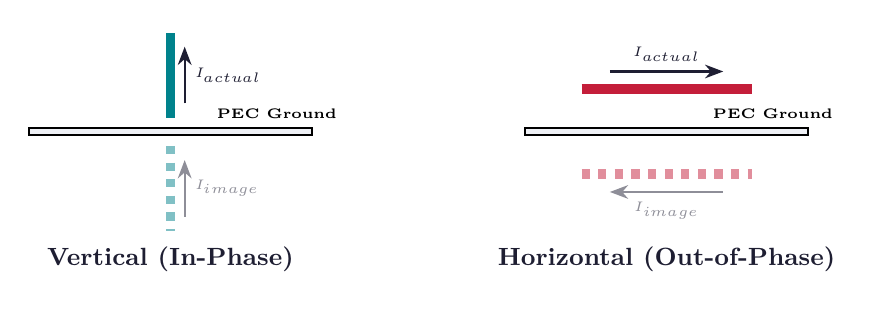
\begin{tikzpicture}[scale=0.9]
  % Vertical antenna case
  \begin{scope}[xshift=-3.5cm]
    \draw[thick, fill=hdrgray] (-2,-0.05) rectangle (2,0.05);
    \node[above, font=\tiny\bfseries] at (1.5,0.05) {PEC Ground};
    
    % Actual dipole
    \draw[line width=3.5pt, color=myteal] (0,0.2) -- (0,1.4);
    \draw[-Stealth, thick, color=mydark] (0.2,0.4) -- (0.2,1.2) node[midway, right, font=\tiny] {$I_{actual}$};
    
    % Image dipole
    \draw[line width=3.5pt, color=myteal!50, dashed] (0,-0.2) -- (0,-1.4);
    \draw[-Stealth, thick, color=mydark!50] (0.2,-1.2) -- (0.2,-0.4) node[midway, right, font=\tiny] {$I_{image}$};
    \node[font=\small\bfseries\color{mydark}] at (0,-1.8) {Vertical (In-Phase)};
  \end{scope}

  % Horizontal antenna case
  \begin{scope}[xshift=3.5cm]
    \draw[thick, fill=hdrgray] (-2,-0.05) rectangle (2,0.05);
    \node[above, font=\tiny\bfseries] at (1.5,0.05) {PEC Ground};
    
    % Actual dipole
    \draw[line width=3.5pt, color=myred] (-1.2,0.6) -- (1.2,0.6);
    \draw[-Stealth, thick, color=mydark] (-0.8,0.85) -- (0.8,0.85) node[midway, above, font=\tiny] {$I_{actual}$};
    
    % Image dipole
    \draw[line width=3.5pt, color=myred!50, dashed] (-1.2,-0.6) -- (1.2,-0.6);
    \draw[Stealth-, thick, color=mydark!50] (-0.8,-0.85) -- (0.8,-0.85) node[midway, below, font=\tiny] {$I_{image}$};
    \node[font=\small\bfseries\color{mydark}] at (0,-1.8) {Horizontal (Out-of-Phase)};
  \end{scope}
\end{tikzpicture}
\end{tcolorbox}

\subsection{Boundary Rules for Image Currents}
\begin{itemize}[leftmargin=*, itemsep=3pt]
  \item \textbf{Vertical Element:} A vertical current element at distance $h$ above a ground plane has an image element of the same length and direction (in-phase) at distance $h$ below the plane.
  \item \textbf{Horizontal Element:} A horizontal current element at distance $h$ above a ground plane has an image element of the same length but opposite direction (out-of-phase) at distance $h$ below the plane.
\end{itemize}

% ===============================================================================
\section{Dipoles for Mobile Communication (Monopoles)}
% ===============================================================================

For mobile handsets and base stations, it is often impractical to use a symmetric double-sided dipole. Instead, a \textbf{monopole antenna} (a single wire placed perpendicular to a conducting ground plane) is used.

\subsection{The Quarter-Wave Monopole (\texorpdfstring{$l = \lambda/4$}{l = lambda/4})}
Using image theory, a monopole of length $l = \lambda/4$ on a perfect ground plane is equivalent to a half-wave dipole ($l = \lambda/2$) in free space, but only for the upper half-space ($z \ge 0$).

\begin{itemize}[leftmargin=*, itemsep=3pt]
  \item \textbf{Fields ($z \ge 0$):} Identical to half-wave dipole fields.
  \item \textbf{Fields ($z < 0$):} Zero (shielded by ground plane).
  \item \textbf{Radiated Power ($P_{rad, mono}$):} Since it radiates only into the upper hemisphere, the radiated power for the same input current is half that of a dipole:
  \[
  P_{rad, monopole} = \frac{1}{2} P_{rad, dipole}
  \]
  \item \textbf{Radiation Resistance ($R_{r, mono}$):}
  \[
  R_{r, monopole} = \frac{1}{2} R_{r, dipole} = \frac{73}{2} \approx 36.5\,\Omega
  \]
  \item \textbf{Directivity ($D_{mono}$):} Since the power is focused into half the volume, the directivity is double that of a dipole:
  \[
  D_{monopole} = 2 \times D_{dipole} = 2 \times 1.64 = 3.28 \quad (5.16\,\text{dBi})
  \]
\end{itemize}

% ===============================================================================
\section{Small Circular Loop Antenna}
% ===============================================================================

\begin{tcolorbox}[defbox, title={\textbf{Definition of Small Circular Loop}}]
A \textbf{small circular loop antenna} is a loop antenna of radius $a$ whose circumference is much smaller than the wavelength ($2\pi a \ll \lambda$), resulting in a uniform current distribution $I(z) = I_0$ along the loop.
\end{tcolorbox}

\subsection{Far-Field Radiated Fields}
By using the magnetic vector potential $\vec{A} = \hat{a}_\phi A_\phi$, the far fields for a loop with area $S = \pi a^2$ are:
\[
E_\phi \approx \frac{\eta k^2 I_0 S \sin\theta}{4\pi r} e^{-jkr}
\]
\[
H_\theta \approx -\frac{E_\phi}{\eta} \approx -\frac{k^2 I_0 S \sin\theta}{4\pi r} e^{-jkr}
\]

\subsection{Radiation Resistance}
The power radiated by the loop is integrated, leading to the radiation resistance:
\[
R_r = 31200 \left( \frac{S}{\lambda^2} \right)^{\!2} = 31200 \left( \frac{\pi a^2}{\lambda^2} \right)^{\!2} \approx 320\pi^4 \left( \frac{a}{\lambda} \right)^{\!4}
\]

\begin{tcolorbox}[defbox, title={\textbf{Important Note: Small Loop as a Magnetic Dipole}}]
The radiation pattern of a small loop has a torus/donut shape ($f(\theta) = \sin\theta$), which is identical to the pattern of an infinitesimal electric dipole. Thus, a small loop behaves as a \textbf{magnetic dipole} perpendicular to the plane of the loop. However, its radiation resistance is much smaller than that of an electric dipole of similar size, making it a less efficient radiator (often used primarily for receiving, e.g., AM radio).
\end{tcolorbox}

% ===============================================================================
% MANDATORY QUICK REVISION PAGE
% ===============================================================================
\newpage
\begin{center}
  {\large\bfseries\color{myred} Quick Revision --- Module 2}\\[3pt]
  {\small\color{mydark} Wire and Loop Antennas $|$ PE-EC801A}
\end{center}
\noindent{\color{myred}\rule{\linewidth}{1.2pt}}
\vspace{4pt}

\begin{tcolorbox}[formulabox, title={\textbf{Key Formulas and Metrics at a Glance}}]
\renewcommand{\arraystretch}{1.35}
\begin{tabularx}{\linewidth}{B{5.2cm} X}
Infinitesimal Dipole $R_r$ & $R_r = 80\pi^2 \left(\frac{dl}{\lambda}\right)^2$ \quad ($dl \ll \lambda$, uniform current) \\[4pt]
Short Dipole $R_r$ & $R_r = 20\pi^2 \left(\frac{l}{\lambda}\right)^2$ \quad ($l \ll \lambda$, linear current) \\[4pt]
Half-Wave Dipole $R_r$ \& $D_0$ & $R_r \approx 73\,\Omega$, \quad $D_0 \approx 1.64$ ($2.15\,\text{dBi}$) \\[4pt]
Quarter-Wave Monopole $R_r$ \& $D_0$ & $R_r \approx 36.5\,\Omega$, \quad $D_0 \approx 3.28$ ($5.16\,\text{dBi}$) \\[4pt]
Small Loop $R_r$ & $R_r \approx 31200 \left(\frac{S}{\lambda^2}\right)^2$ \quad ($S = \pi a^2$) \\[4pt]
Dipole Current Profile & $I(z) = I_0 \sin\left[k(l/2 - |z|)\right]$ \\[4pt]
Resonant Dipole Length & $l_{resonant} \approx 0.47\lambda$–$0.48\lambda$ \quad (removes $+j42.5\,\Omega$ reactance) \\
\end{tabularx}
\end{tcolorbox}

\begin{tcolorbox}[defbox, title={\textbf{One-Line Definitions}}]
\begin{itemize}[leftmargin=*, itemsep=2pt, topsep=0pt]
  \item \textbf{Hertzian Dipole:} A theoretical, infinitely thin dipole antenna of length much smaller than a wavelength, carrying uniform current.
  \item \textbf{Resonant Antenna:} An antenna whose input impedance is purely resistive ($X_{in} = 0$) at its operating frequency.
  \item \textbf{Image Theory:} A mathematical method replacing a conducting boundary with virtual mirror-image current sources.
  \item \textbf{Quarter-Wave Monopole:} A single vertical wire of length $\lambda/4$ placed above a conducting ground plane.
  \item \textbf{Magnetic Dipole:} The dual of an electric dipole; represented physically by a small circular loop antenna.
\end{itemize}
\end{tcolorbox}

\begin{tcolorbox}[exambox, title={\textbf{Frequently Asked / Viva Questions}}]
\begin{enumerate}[topsep=0pt, label=\textbf{Q\arabic*.}, itemsep=5pt]
  \item \Q{What is the difference between an infinitesimal dipole and a short dipole?}
    An infinitesimal dipole has a constant, uniform current along its length ($dl \ll \lambda$). A short dipole has current that drops off linearly from the center to zero at the ends ($l \ll \lambda$). Because of this current profile, the radiation resistance of a short dipole is one-quarter of that of an infinitesimal dipole.
  \item \Q{Why does a half-wave dipole require shortening for resonance?}
    A physical half-wave dipole ($l = 0.5\lambda$) has an input impedance of $Z_{in} \approx 73 + j42.5\,\Omega$. To eliminate the inductive reactance and make it resonant ($X_{in} = 0$), the antenna is shortened slightly to about $0.47\lambda$–$0.48\lambda$.
  \item \Q{Compare a half-wave dipole and a quarter-wave monopole antenna.}
    A quarter-wave monopole on a ground plane has half the radiation resistance ($36.5\,\Omega$ vs. $73\,\Omega$) and twice the directivity ($3.28$ vs. $1.64$, or $5.16\,\text{dBi}$ vs. $2.15\,\text{dBi}$) of a free-space half-wave dipole, because its radiation is restricted to the upper hemisphere.
  \item \Q{Explain how the image of a horizontal dipole differs from a vertical dipole.}
    For a vertical dipole, the image current is in the same direction (in-phase). For a horizontal dipole, the image current is in the opposite direction (out-of-phase), which causes the radiated field to cancel at grazing angles ($0^\circ$ elevation).
  \item \Q{Why are small loop antennas rarely used as transmitting antennas?}
    Small loop antennas have a very small radiation resistance (proportional to $(a/\lambda)^4$). This makes their radiation efficiency extremely low, as most input power is lost as heat in the conductor. They are, however, excellent for receiving applications (like AM radio) where noise levels are high and matching can be tuned.
  \item \Q{Write the far-field expressions for a half-wave dipole.}
    $E_\theta = j 120 I_0 \frac{e^{-jkr}}{2 r} \left[ \frac{\cos\left(\frac{\pi}{2}\cos\theta\right)}{\sin\theta} \right]$ and $H_\phi = \frac{E_\theta}{\eta}$. Other field components are zero.
  \item \Q{What is the input impedance of a practical half-wave dipole at resonance?}
    At resonance, the input reactance is tuned to zero, and the input impedance is purely resistive: $Z_{in} \approx 73\,\Omega$.
\end{enumerate}
\end{tcolorbox}

\begin{tcolorbox}[tikzbox, title={Comparison of Wire and Loop Antennas}]
\centering
\renewcommand{\arraystretch}{1.55}
{\renewcommand{\arraystretch}{1.55}%
\begin{tabularx}{\linewidth}{|B{3.2cm}|Y|Y|Y|}
\hline
\multicolumn{1}{|>{\centering\arraybackslash}m{3.2cm}|}{\textbf{Parameter}} &
\multicolumn{1}{>{\centering\arraybackslash}Y|}{\textbf{Hertzian Dipole}} &
\multicolumn{1}{>{\centering\arraybackslash}Y|}{\textbf{Half-Wave Dipole}} &
\multicolumn{1}{>{\centering\arraybackslash}Y|}{\textbf{Small Loop}} \\
\hline
Length / Size & $dl \ll \lambda$ & $l = \lambda/2$ & Radius $a \ll \lambda / 2\pi$ \\
\hline
Current Profile & Uniform ($I_0$) & Sinusoidal ($I_0 \cos kz$) & Uniform ($I_0$) \\
\hline
Radiation Resistance & $80\pi^2 (dl/\lambda)^2$ & $73\,\Omega$ & $31200 (\pi a^2/\lambda^2)^2$ \\
\hline
Directivity & $1.5$ ($1.76\,\text{dBi}$) & $1.64$ ($2.15\,\text{dBi}$) & $1.5$ ($1.76\,\text{dBi}$) \\
\hline
Field Type & Electric Dipole & Finite Electric Dipole & Magnetic Dipole \\
\hline
\end{tabularx}}
\end{tcolorbox}


% -- Module 3 -----------------------------------------------------------------
\modulestart{3}{Huygens' Principle and Field Equivalence}

\section{Huygens' Principle and Field Equivalence}
% ===============================================================================

\begin{tcolorbox}[defbox, title={\textbf{Huygens' Principle}}]
\textbf{Huygens' Principle} states that each point on a primary wavefront behaves as a source of secondary spherical wavelets. These wavelets propagate outward at the speed of the wave in the medium, and the new wavefront at any subsequent time is the envelope of these secondary wavelets.
\end{tcolorbox}

\subsection{Field Equivalence Principle}
In electromagnetics, Schelkunoff's Equivalence Principle allows us to replace actual source currents inside a closed surface $S$ with equivalent electric ($\vec{J}_s$) and magnetic ($\vec{M}_s$) currents on the surface $S$ such that the fields outside $S$ remain unchanged:
\[
\vec{J}_s = \hat{n} \times \vec{H}
\]
\[
\vec{M}_s = -\hat{n} \times \vec{E}
\]
where $\hat{n}$ is the unit outward normal vector to the surface $S$, and $\vec{E}$, $\vec{H}$ are the fields on $S$. This is critical for solving radiation patterns of aperture antennas.

\begin{tcolorbox}[tikzbox, title={Huygens' Wavelet Propagation}]
\centering
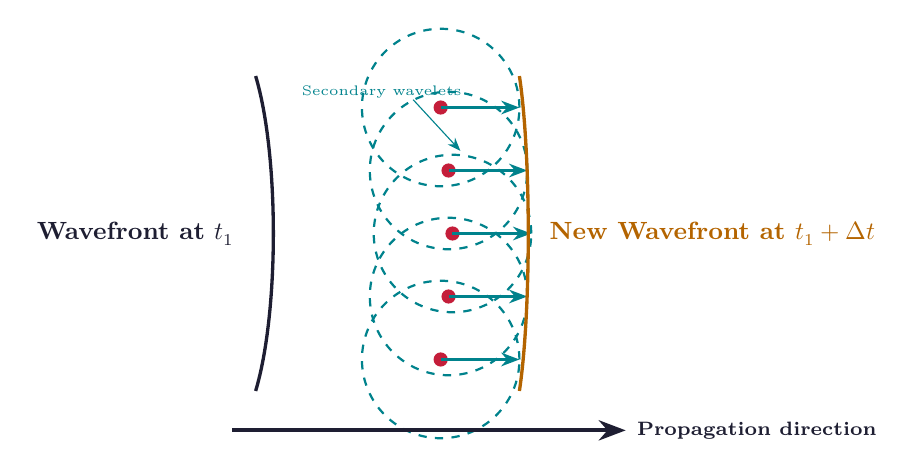
\begin{tikzpicture}[scale=1.0]
  % ── Original wavefront (left, slightly curved) ────────────────────────────
  \draw[very thick, color=mydark] (-2.5,-2.0) .. controls (-2.2,-1.0) and (-2.2,1.0) .. (-2.5,2.0);
  \node[left=4pt, align=right, font=\small\bfseries\color{mydark}] at (-2.5,0) {Wavefront at $t_1$};

  % ── Secondary wavelet sources (5 points on the primary wavefront) ──────────
  \foreach \y/\xo in {-1.6/-0.15, -0.8/-0.05, 0.0/0.0, 0.8/-0.05, 1.6/-0.15} {
    % Source dot
    \fill[myred] (\xo, \y) circle (0.09);
    % Wavelet circle
    \draw[color=myteal, dashed, line width=0.8pt] (\xo, \y) circle (1.0);
    % Arrow showing propagation direction
    \draw[-Stealth, color=myteal, thick] (\xo, \y) -- ++(1.0, 0);
  }

  % ── New wavefront envelope (right, tangent to all wavelets) ─────────────────
  \draw[very thick, color=myamber]
    (0.85,-2.0) .. controls (1.0,-1.0) and (1.0,1.0) .. (0.85,2.0);

  % ── Labels ────────────────────────────────────────────────────────────────
  \node[right=6pt, align=left, font=\small\bfseries\color{myamber}] at (0.9, 0) {New Wavefront at $t_1 + \Delta t$};
  \node[font=\tiny\color{myteal}] at (-0.9, 1.8) {Secondary wavelets};
  \draw[-Stealth, thin, color=myteal] (-0.5, 1.7) -- (0.1, 1.05);

  % ── Propagation direction arrow ────────────────────────────────────────────
  \draw[-Stealth, line width=1.5pt, color=mydark] (-2.8, -2.5) -- (2.2, -2.5)
    node[right, font=\scriptsize\bfseries] {Propagation direction};
\end{tikzpicture}
\end{tcolorbox}

% ===============================================================================
\section{Radiation from Apertures}
% ===============================================================================

Aperture antennas (like waveguides, horns, and reflectors) radiate through an opening in their structure. The radiated fields in the far field are proportional to the spatial Fourier transform of the field distribution across the aperture.

\subsection{Rectangular Aperture (Uniform Distribution)}
Consider a rectangular aperture of dimensions $a$ (along $x$) and $b$ (along $y$) in an infinite ground plane. If the aperture field is uniform and $x$-polarized, $\vec{E}_a = \hat{a}_x E_0$, the far-field pattern is:
\[
E(\theta, \phi) \propto \text{sinc}\left( \frac{ka}{2} \sin\theta \cos\phi \right) \text{sinc}\left( \frac{kb}{2} \sin\theta \sin\phi \right)
\]
where $\text{sinc}(x) = \frac{\sin x}{x}$.
\begin{itemize}[leftmargin=*, itemsep=3pt]
  \item \textbf{Maximum Directivity:}
  \[
  D_{max} = \frac{4\pi}{\lambda^2} A_p = \frac{4\pi}{\lambda^2} (ab)
  \]
  \item \textbf{Beamwidth (HPBW):}
  \[
  \text{HPBW}_{E\text{-plane}} \approx 50.6^\circ \frac{\lambda}{b}, \quad \text{HPBW}_{H\text{-plane}} \approx 50.6^\circ \frac{\lambda}{a}
  \]
\end{itemize}

\subsection{Circular Aperture (Uniform Distribution)}
For a circular aperture of radius $a$ with a uniform field, the far-field pattern is described by a Bessel function:
\[
E(\theta) \propto \frac{J_1(ka \sin\theta)}{ka \sin\theta}
\]
where $J_1$ is the first-order Bessel function.
\begin{itemize}[leftmargin=*, itemsep=3pt]
  \item \textbf{Maximum Directivity:}
  \[
  D_{max} = \frac{4\pi}{\lambda^2} A_p = \frac{4\pi}{\lambda^2} (\pi a^2) = \left( \frac{2\pi a}{\lambda} \right)^{\!2}
  \]
  \item \textbf{First Null Angle:} $\theta_{null} \approx 1.22 \frac{\lambda}{2a}$.
  \item \textbf{First Sidelobe Level:} $17.6\,\text{dB}$ below the main beam peak.
\end{itemize}

% ===============================================================================
\section{Babinet's Principle and Slot Antennas}
% ===============================================================================

\subsection{Babinet's Principle}
In optics, Babinet's Principle states that the sum of the diffraction fields behind two complementary screens (where the transparent areas of one screen correspond to the opaque areas of the other) equals the field of the source when no screen is present.

\subsection{Electromagnetic Extension (Booker's Relation)}
H. G. Booker extended Babinet's principle to account for electromagnetic vector properties (polarization and boundary conditions). It relates the input impedance of a slot antenna ($Z_{slot}$) to the impedance of its complementary metal strip dipole ($Z_{dipole}$):

\begin{tcolorbox}[formulabox, title={\textbf{Booker's Impedance Relation}}]
For complementary slot and dipole antennas in free space:
\[
Z_{slot} Z_{dipole} = \frac{\eta_0^2}{4}
\]
where $\eta_0 \approx 377\,\Omega \approx 120\pi$ is the intrinsic impedance of free space.
\end{tcolorbox}

Substituting $\eta_0 \approx 120\pi$:
\[
Z_{slot} Z_{dipole} = \frac{(120\pi)^2}{4} \approx 35476\,\Omega^2
\]
\textbf{Implications:}
\begin{itemize}[leftmargin=*, itemsep=3pt]
  \item Since a resonant thin dipole has $Z_{dipole} \approx 73\,\Omega$, its complementary slot antenna has a resonant input impedance of:
  \[
  Z_{slot} = \frac{35476}{73} \approx 485\,\Omega
  \]
  \item The polarization of the slot antenna is orthogonal to that of the dipole. A vertical slot antenna radiates horizontally polarized waves, whereas a vertical dipole radiates vertically polarized waves.
\end{itemize}

% ===============================================================================
\section{Horn Antennas}
% ===============================================================================

A \textbf{horn antenna} is a flared waveguide that provides a smooth transition from waveguide impedance to free-space impedance, producing high directivity.

\subsection{Types of Horns}
\begin{itemize}[leftmargin=*, itemsep=3pt]
  \item \textbf{E-Plane Sectoral Horn:} Flared only in the direction of the electric field ($E$-field).
  \item \textbf{H-Plane Sectoral Horn:} Flared only in the direction of the magnetic field ($H$-field).
  \item \textbf{Pyramidal Horn:} Flared in both E and H directions. It has a rectangular aperture.
  \item \textbf{Conical Horn:} Circular waveguide flared into a cone.
\end{itemize}

\begin{tcolorbox}[tikzbox, title={Horn Antenna Structures}]
\centering
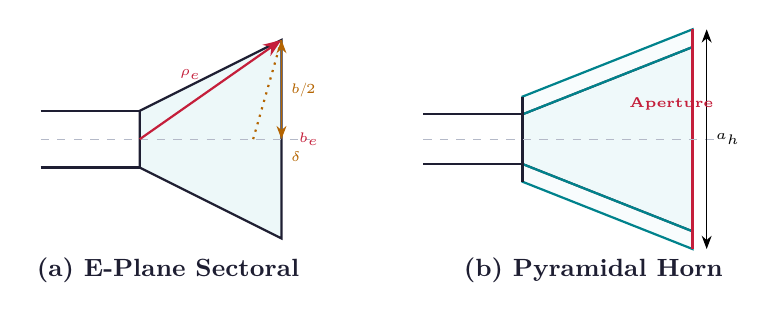
\begin{tikzpicture}[scale=0.9]
  % ── (a) E-Plane Sectoral Horn ──────────────────────────────────────────────
  \begin{scope}[xshift=-4.2cm]
    % Waveguide walls (side view)
    \draw[thick, color=mydark] (-2.0, 0.4) -- (-0.6, 0.4);
    \draw[thick, color=mydark] (-2.0, -0.4) -- (-0.6, -0.4);
    % Flared aperture (E-plane flares vertically)
    \draw[thick, color=mydark, fill=hdrteal, fill opacity=0.5]
      (-0.6, 0.4) -- (1.4, 1.4) -- (1.4, -1.4) -- (-0.6, -0.4) -- cycle;
    % Back wall
    \draw[thick, color=mydark] (-0.6, 0.4) -- (-0.6, -0.4);
    % Center axis
    \draw[dashed, color=mgframe] (-2.0, 0) -- (1.8, 0);
    % Slant length annotation
    \draw[color=myred, -Stealth, thick] (-0.6,0) -- (1.4,1.4) node[midway, above left, font=\tiny] {$\rho_e$};
    % Path difference
    \draw[Stealth-Stealth, thin, color=myamber] (1.4,0) -- (1.4,1.4) node[midway, right, font=\tiny] {$b/2$};
    % Aperture label
    \node[right=3pt, font=\tiny\bfseries\color{myred}] at (1.4, 0) {$b_e$};
    \node[font=\small\bfseries\color{mydark}] at (-0.2,-1.85) {(a) E-Plane Sectoral};
    % Phase error arrows
    \draw[dotted, thick, color=myamber] (1.0,0) -- (1.4, 1.4);
    \node[font=\tiny\color{myamber}] at (1.6,-0.25) {$\delta$};
  \end{scope}

  % ── (b) Pyramidal Horn ─────────────────────────────────────────────────────
  \begin{scope}[xshift=1.4cm]
    % Front face waveguide (top)
    \draw[thick, color=mydark] (-0.8, 0.35) -- (-2.2, 0.35);
    \draw[thick, color=mydark] (-0.8, -0.35) -- (-2.2, -0.35);
    % Left side flap (H-plane)
    \draw[thick, color=mydark] (-0.8, 0.35) -- (-2.2, 0.35);
    % Pyramid outline (top view approximation)
    % Top face
    \draw[thick, color=mydark, fill=hdrteal, fill opacity=0.45]
      (-0.8, 0.35) -- (1.6, 1.3) -- (1.6, -1.3) -- (-0.8, -0.35) -- cycle;
    % H-plane (width) flare shown as offset overlay
    \draw[thick, color=myteal, fill=hdrteal, fill opacity=0.2]
      (-0.8, 0.35) -- (-0.8, 0.6) -- (1.6, 1.55) -- (1.6, 1.3) -- cycle;
    \draw[thick, color=myteal, fill=hdrteal, fill opacity=0.2]
      (-0.8, -0.35) -- (-0.8, -0.6) -- (1.6, -1.55) -- (1.6, -1.3) -- cycle;
    % Aperture lip
    \draw[very thick, color=myred] (1.6, -1.55) -- (1.6, 1.55);
    % Back wall
    \draw[thick, color=mydark] (-0.8, 0.6) -- (-0.8, -0.6);
    \draw[thick, color=mydark] (-2.2, 0.35) -- (-0.8, 0.35);
    \draw[thick, color=mydark] (-2.2, -0.35) -- (-0.8, -0.35);
    % Axis
    \draw[dashed, color=mgframe] (-2.2, 0) -- (2.0, 0);
    % Dimension labels
    \draw[Stealth-Stealth, thin] (1.8, -1.55) -- (1.8, 1.55) node[midway, right, font=\tiny] {$a_h$};
    \node[font=\small\bfseries\color{mydark}] at (0.2,-1.85) {(b) Pyramidal Horn};
    \node[font=\tiny\bfseries\color{myred}] at (1.3,0.5) {Aperture};
  \end{scope}
\end{tikzpicture}
\end{tcolorbox}

\subsection{Design Concepts and Path Length Difference}
Flaring the waveguide causes a phase variation across the horn's aperture because waves traveling to the outer edge of the horn travel a longer path length ($\rho$) than waves traveling along the center axis. 
The maximum path difference $\delta$ is:
\[
\delta = \rho \left( 1 - \cos\frac{\theta}{2} \right) \approx \frac{b^2}{8\rho}
\]
where $b$ is the aperture height and $\rho$ is the horn length.
To prevent destructive interference, $\delta$ must be kept within limit:
\begin{itemize}[leftmargin=*, itemsep=2pt]
  \item For $E$-plane horn: $\delta_{max} < \lambda / 4 \implies b^2 < 2 \lambda \rho_e$.
  \item For $H$-plane horn: $\delta_{max} < 3\lambda / 8 \implies a^2 < 3 \lambda \rho_h$.
\end{itemize}

% ===============================================================================
\section{Reflector Antennas}
% ===============================================================================

Reflector antennas use a metallic surface to redirect and focus electromagnetic waves from a primary source (feed) into a highly directive beam.

\subsection{Prime-Focus Parabolic Reflector}
A paraboloidal reflector is a surface of revolution formed by rotating a parabola about its axis. A primary feed (e.g., dipole or small horn) is placed at the focal point $F$.

\begin{tcolorbox}[tikzbox, title={Parabolic Reflector Configurations}]
\centering
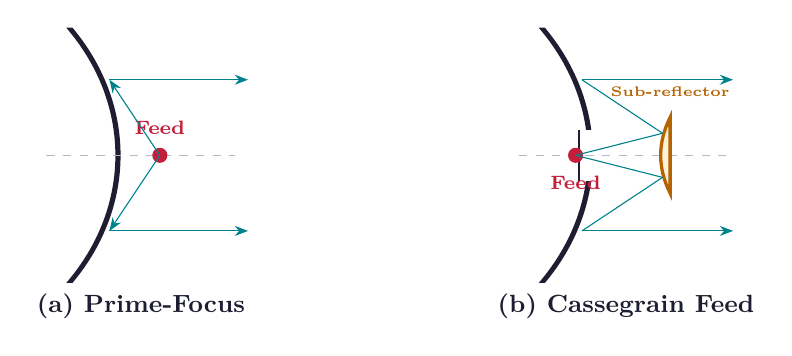
\begin{tikzpicture}[scale=0.8]
  % Prime Focus Reflector
  \begin{scope}[xshift=-4cm]
    % Draw parabola
    \draw[very thick, color=mydark, fill=hdrgray] 
      (-0.8, 2.0) .. controls (0.2, 0.8) and (0.2, -0.8) .. (-0.8, -2.0) -- 
      (-0.83, -2.0) .. controls (0.17, -0.8) and (0.17, 0.8) .. (-0.83, 2.0) -- cycle;
      
    % Axis
    \draw[dashed, color=mgframe] (-1.2, 0) -- (1.8, 0);
    
    % Focal point feed
    \fill[myred] (0.6, 0) circle (0.12) node[above=4pt, font=\scriptsize\bfseries] {Feed};
    
    % Ray tracing
    \draw[color=myteal, -Stealth] (0.6,0) -- (-0.2, 1.2);
    \draw[color=myteal, -Stealth] (-0.2, 1.2) -- (2.0, 1.2);
    \draw[color=myteal, -Stealth] (0.6,0) -- (-0.2, -1.2);
    \draw[color=myteal, -Stealth] (-0.2, -1.2) -- (2.0, -1.2);
    
    \node[font=\small\bfseries\color{mydark}] at (0.3,-2.4) {(a) Prime-Focus};
  \end{scope}

  % Cassegrain Reflector
  \begin{scope}[xshift=3.5cm]
    % Draw main parabola
    \draw[very thick, color=mydark, fill=hdrgray] 
      (-0.8, 2.0) .. controls (0.2, 0.8) and (0.2, -0.8) .. (-0.8, -2.0) -- 
      (-0.83, -2.0) .. controls (0.17, -0.8) and (0.17, 0.8) .. (-0.83, 2.0) -- cycle;
      
    % Hole in main reflector
    \fill[white] (-0.35, -0.4) rectangle (0.05, 0.4);
    \draw[thick, color=mydark] (-0.25, 0.4) -- (-0.25, -0.4);
    
    % Axis
    \draw[dashed, color=mgframe] (-1.2, 0) -- (2.2, 0);
    
    % Sub-reflector (hyperbolic)
    \draw[very thick, color=myamber, fill=hdramber] 
      (1.2, 0.6) .. controls (1.0, 0.2) and (1.0, -0.2) .. (1.2, -0.6) -- cycle;
    \node[above=4pt, font=\tiny\bfseries\color{myamber}] at (1.2, 0.6) {Sub-reflector};
      
    % Actual feed at vertex
    \fill[myred] (-0.3, 0) circle (0.12) node[below=4pt, font=\scriptsize\bfseries] {Feed};
    
    % Rays
    \draw[color=myteal] (-0.3,0) -- (1.08, 0.35);
    \draw[color=myteal] (1.08, 0.35) -- (-0.2, 1.2);
    \draw[color=myteal, -Stealth] (-0.2, 1.2) -- (2.2, 1.2);
    
    \draw[color=myteal] (-0.3,0) -- (1.08, -0.35);
    \draw[color=myteal] (1.08, -0.35) -- (-0.2, -1.2);
    \draw[color=myteal, -Stealth] (-0.2, -1.2) -- (2.2, -1.2);
    
    \node[font=\small\bfseries\color{mydark}] at (0.5,-2.4) {(b) Cassegrain Feed};
  \end{scope}
\end{tikzpicture}
\end{tcolorbox}

\textbf{Characteristics:}
\begin{itemize}[leftmargin=*, itemsep=3pt]
  \item Converts a spherical wavefront radiating from the feed into a highly directive plane wavefront.
  \item All path lengths from the feed to the reflector and out to the aperture plane are identical: $r + r\cos\theta = 2f$.
  \item The $f/D$ ratio (focal length to diameter) is a critical design parameter that determines the curvature of the dish and feed antenna illumination requirements.
  \item \textbf{Gain:} The power gain of a parabolic reflector of diameter $D$ with aperture efficiency $\eta_{ap}$ is:
  \[
  G = \eta_{ap} \left( \frac{\pi D}{\lambda} \right)^{\!2}
  \]
  where $\eta_{ap} \approx 0.5$–$0.7$ for practical dishes (accounts for spillover, illumination taper, phase errors, and blockage). For a typical $\eta_{ap} = 0.55$: a 3 m dish at 10 GHz gives $G \approx 3 \times 10^4$ ($\approx 45\,\text{dBi}$).\end{itemize}

\subsection{Cassegrain Antenna (Dual-Reflector)}
A \textbf{Cassegrain antenna} uses a primary parabolic main reflector and a secondary hyperbolic sub-reflector.
\begin{itemize}[leftmargin=*, itemsep=3pt]
  \item \textbf{Setup:} The primary feed horn is placed at a convenient location, usually at the vertex of the main reflector. The sub-reflector is positioned between the feed and the main focus.
  \item \textbf{Ray Path:} Spherical waves from the feed are reflected by the hyperbolic sub-reflector, directing them toward the main parabolic reflector as if they originated from the paraboloid's focus. The main reflector then reflects them as a collimated plane wave.
\end{itemize}

\par\noindent
\textbf{Cassegrain Advantages:}\par\noindent
{\renewcommand{\arraystretch}{1.45}%
\begin{tabularx}{\linewidth}{|B{3.5cm}|Y|}
\hline
\textbf{Feature} & \textbf{Cassegrain Advantage} \\
\hline
Feed Line Loss & Feed is at the vertex; eliminates long, lossy feed lines to the focus. \\
\hline
Noise Temperature & Feed looks up at the cold sky (via sub-reflector) rather than down at the warm, noisy earth, reducing receiver noise. \\
\hline
Structural Support & Heavy feed equipment (amplifiers, cryogenics) is mounted behind the dish, rather than being suspended at the focus. \\
\hline
\end{tabularx}}

% ===============================================================================
% MANDATORY QUICK REVISION PAGE
% ===============================================================================
\newpage
\begin{center}
  {\large\bfseries\color{myred} Quick Revision --- Module 3}\\[3pt]
  {\small\color{mydark} Aperture and Reflector Antennas $|$ PE-EC801A}
\end{center}
\noindent{\color{myred}\rule{\linewidth}{1.2pt}}
\vspace{4pt}

\begin{tcolorbox}[formulabox, title={\textbf{Key Formulas and Metrics at a Glance}}]
\renewcommand{\arraystretch}{1.35}
\begin{tabularx}{\linewidth}{B{5.2cm} X}
Aperture Max Directivity & $D_{max} = \frac{4\pi}{\lambda^2} A_p$ \quad (uniform distribution) \\[4pt]
Circular Apertity Null & $\theta_{null} \approx 1.22 \frac{\lambda}{2a}$ \\[4pt]
Booker's Relation & $Z_{slot} Z_{dipole} = \frac{\eta_0^2}{4} \approx 35476\,\Omega^2$ \\[4pt]
Resonant Slot Impedance & $Z_{slot} \approx 485\,\Omega$ \quad (complementary to $73\,\Omega$ dipole) \\[4pt]
Parabolic Reflector Gain & $G = \eta_{ap} \left(\frac{\pi D}{\lambda}\right)^2$ \quad ($\eta_{ap} \approx 0.55$) \\[4pt]
Horn Flare Limit (E-plane) & $b^2 < 2\lambda\rho_e$ \quad (limits phase error to $< \pi/2$) \\[4pt]
Horn Flare Limit (H-plane) & $a^2 < 3\lambda\rho_h$ \quad (limits phase error to $< 3\pi/4$) \\[4pt]
Parabola Equation & $y^2 = 4fx$ \quad ($f$ = focal length) \\
\end{tabularx}
\end{tcolorbox}

\begin{tcolorbox}[defbox, title={\textbf{One-Line Definitions}}]
\begin{itemize}[leftmargin=*, itemsep=2pt, topsep=0pt]
  \item \textbf{Equivalence Principle:} A principle allowing actual source fields inside a closed boundary to be replaced by equivalent surface currents.
  \item \textbf{Aperture Efficiency:} The ratio of the effective aperture of an antenna to its physical aperture area.
  \item \textbf{Complementary Screens:} Two screens where the open areas of one correspond to the closed areas of the other.
  \item \textbf{Optimum Horn:} A horn antenna whose dimensions are chosen to achieve maximum gain for a fixed flare length.
  \item \textbf{Spillover Loss:} Power radiated by the feed antenna that misses the reflector dish and is lost.
  \item \textbf{Cassegrain Antenna:} A dual-reflector system using a parabolic main reflector and a hyperbolic sub-reflector.
\end{itemize}
\end{tcolorbox}

\begin{tcolorbox}[exambox, title={\textbf{Frequently Asked / Viva Questions}}]
\begin{enumerate}[topsep=0pt, label=\textbf{Q\arabic*.}, itemsep=5pt]
  \item \Q{State Babinet's principle and its electromagnetic extension (Booker's relation).}
    Babinet's principle states that the sum of the fields behind complementary screens equals the source field without screens. Booker's relation extends this to EM fields, showing that for a slot antenna and its complementary dipole, $Z_{slot} Z_{dipole} = \frac{\eta_0^2}{4}$.
  \item \Q{Why does a slot antenna have a high input impedance compared to a dipole?}
    By Booker's relation, $Z_{slot} Z_{dipole} \approx 35476$. Because a resonant dipole has $Z_{dipole} \approx 73\,\Omega$, its complementary slot antenna has a high impedance: $Z_{slot} = \frac{35476}{73} \approx 485\,\Omega$.
  \item \Q{Compare the polarization of a vertical slot antenna and a vertical dipole.}
    They are orthogonal. A vertical dipole radiates vertically polarized waves, whereas a vertical slot antenna radiates horizontally polarized waves (because the electric field lines span horizontally across the vertical slot).
  \item \Q{Why are horn antennas flared? What happens if the flare angle is too large?}
    Flaring provides a gradual impedance match from the waveguide to free space, reducing reflections. If the flare angle is too large, the path difference between central and edge rays becomes large, causing phase errors that degrade gain and increase sidelobes.
  \item \Q{What are the advantages of a Cassegrain reflector over a prime-focus parabolic reflector?}
    \begin{itemize}[leftmargin=*, itemsep=1pt, topsep=2pt]
      \item Lower transmission line loss because the feed is located at the vertex.
      \item Lower noise temperature since the feed points upward at the cold sky.
      \item Easy installation and maintenance of heavy feed and receiver electronics.
    \end{itemize}
  \item \Q{Explain the trade-off involved in the $f/D$ ratio of a parabolic reflector.}
    A small $f/D$ (deep dish) reduces spillover but requires a wide-angle feed, which is hard to design with uniform phase. A large $f/D$ (flat dish) simplifies feed design but increases spillover loss and requires a longer, heavier feed structure.
  \item \Q{State the field equivalence principle and its use in aperture antennas.}
    It allows replacing the actual sources inside a closed surface with equivalent electric and magnetic currents on the surface. It simplifies analyzing slot, horn, or aperture antennas by integrating fields across the aperture rather than calculating currents on complex conductors.
\end{enumerate}
\end{tcolorbox}

\begin{tcolorbox}[tikzbox, title={Comparison of Aperture Antenna Types}]
\centering
\renewcommand{\arraystretch}{1.55}
{\renewcommand{\arraystretch}{1.55}%
\begin{tabularx}{\linewidth}{|B{3.0cm}|Y|Y|Y|}
\hline
\multicolumn{1}{|>{\centering\arraybackslash}m{3.0cm}|}{\textbf{Parameter}} &
\multicolumn{1}{>{\centering\arraybackslash}Y|}{\textbf{Slot Antenna}} &
\multicolumn{1}{>{\centering\arraybackslash}Y|}{\textbf{Horn Antenna}} &
\multicolumn{1}{>{\centering\arraybackslash}Y|}{\textbf{Parabolic Reflector}} \\
\hline
Directivity / Gain & Low to Medium & Medium ($10$–$25\,\text{dB}$) & Very High ($30$–$50\,\text{dB}$) \\
\hline
Bandwidth & Narrow (resonant) & Wide (waveguide band) & Extremely Wide \\
\hline
Impedance & High ($\approx 485\,\Omega$) & Matched to waveguide & Matches feed antenna \\
\hline
Typical Applications & Aircraft, radar arrays & Feed for reflectors, gain standards & Satellite TV, radar, radio astronomy \\
\hline
\end{tabularx}}
\end{tcolorbox}


% -- Module 4 -----------------------------------------------------------------
\modulestart{4}{Yagi-Uda Antenna}

\section{Yagi-Uda Antenna}
% ===============================================================================

\begin{tcolorbox}[defbox, title={\textbf{Definition of Yagi-Uda Antenna}}]
The \textbf{Yagi-Uda antenna} is a highly directional, narrow-band antenna consisting of a single driven element (usually a half-wave folded dipole) and one or more parasitic elements (a reflector behind it, and directors in front of it) aligned along a central supporting boom.
\end{tcolorbox}

\subsection{Structure and Elements}
The parasitic elements are not connected to the feed line. They receive energy through mutual electromagnetic coupling from the driven element and re-radiate it.

\begin{tcolorbox}[tikzbox, title={Yagi-Uda Antenna Layout}]
\centering
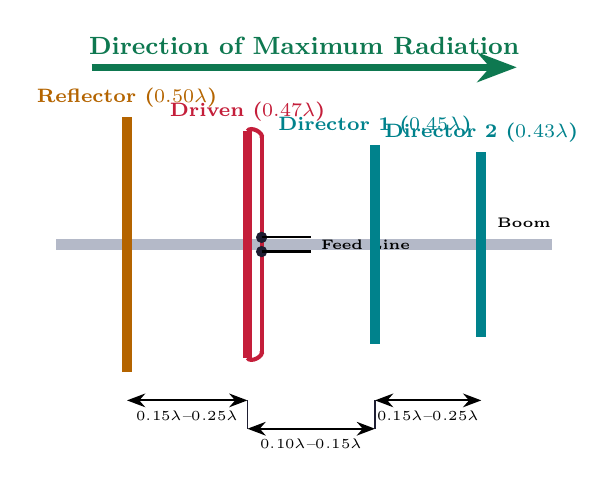
\begin{tikzpicture}[scale=0.9]
  % Supporting Boom
  \draw[line width=4pt, color=mgframe] (-3.5,0) -- (3.5,0);
  \node[above, font=\tiny\bfseries] at (3.1,0.1) {Boom};

  % Reflector
  \draw[line width=3.5pt, color=myamber] (-2.5,-1.8) -- (-2.5,1.8);
  \node[above, font=\scriptsize\bfseries\color{myamber}] at (-2.5,1.8) {Reflector ($0.50\lambda$)};

  % Driven Element (Folded Dipole sketch)
  \draw[line width=3.5pt, color=myred] (-0.8,-1.6) -- (-0.8,1.6);
  \draw[line width=1.5pt, color=myred] (-0.6,-1.5) -- (-0.6,1.5);
  \draw[line width=1.5pt, color=myred] (-0.8,1.6) to[bend left=90] (-0.6,1.5);
  \draw[line width=1.5pt, color=myred] (-0.8,-1.6) to[bend right=90] (-0.6,-1.5);
  \fill[mydark] (-0.6, 0.1) circle (0.08);
  \fill[mydark] (-0.6, -0.1) circle (0.08);
  \draw[thick] (-0.6,0.1) -- (0.1,0.1);
  \draw[thick] (-0.6,-0.1) -- (0.1,-0.1);
  \node[right, font=\tiny\bfseries] at (0.1,0) {Feed Line};
  \node[above, font=\scriptsize\bfseries\color{myred}] at (-0.8,1.6) {Driven ($0.47\lambda$)};

  % Directors
  \draw[line width=3.5pt, color=myteal] (1.0,-1.4) -- (1.0,1.4);
  \node[above, font=\scriptsize\bfseries\color{myteal}] at (1.0,1.4) {Director 1 ($0.45\lambda$)};

  % Director 2
  \draw[line width=3.5pt, color=myteal] (2.5,-1.3) -- (2.5,1.3);
  \node[above, font=\scriptsize\bfseries\color{myteal}] at (2.5,1.3) {Director 2 ($0.43\lambda$)};

  % Spacing dimension lines — staggered vertically to prevent overlap
  \draw[Stealth-Stealth, thick] (-2.5, -2.2) -- (-0.8, -2.2)
    node[midway, below, font=\tiny] {$0.15\lambda$–$0.25\lambda$};
  \draw[Stealth-Stealth, thick] (-0.8, -2.6) -- (1.0, -2.6)
    node[midway, below, font=\tiny] {$0.10\lambda$–$0.15\lambda$};
  \draw[Stealth-Stealth, thick] (1.0, -2.2) -- (2.5, -2.2)
    node[midway, below, font=\tiny] {$0.15\lambda$–$0.25\lambda$};
  % Connector lines for staggered middle arrow
  \draw[thin, color=mydark] (-0.8,-2.2) -- (-0.8,-2.6);
  \draw[thin, color=mydark] (1.0,-2.2) -- (1.0,-2.6);

  % Radiation Direction Arrow
  \draw[-Stealth, line width=2.5pt, color=mygreen] (-3.0, 2.5) -- (3.0, 2.5) 
    node[midway, above, font=\small\bfseries] {Direction of Maximum Radiation};
\end{tikzpicture}
\end{tcolorbox}

\begin{enumerate}[label=\textbf{\arabic*.}, leftmargin=*, itemsep=4pt]
  \item \textbf{Driven Element:} Typically a folded dipole of resonant length $0.47\lambda$–$0.48\lambda$. The folded dipole structure increases the input impedance from $73\,\Omega$ to around $300\,\Omega$, facilitating impedance matching with standard twin-lead transmission lines.
  \item \textbf{Reflector:} Placed behind the driven element. It is approximately $5\%$ longer than the driven element ($\approx 0.50\lambda$) and spaced $0.15\lambda$–$0.25\lambda$ away. Because it is longer, it is inductive. It redirects the wave in the forward direction.
  \item \textbf{Directors:} Placed in front of the driven element in the direction of the main beam. They are $5\%$ shorter than the driven element ($\approx 0.40\lambda$–$0.45\lambda$) and spaced $0.10\lambda$–$0.30\lambda$ apart. Because they are shorter, they are capacitive, directing wave propagation forward.
\end{enumerate}

\subsection{Characteristics}
\begin{itemize}[leftmargin=*, itemsep=2pt]
  \item \textbf{Directivity/Gain:} Typically $7$–$15\,\text{dB}$ depending on the number of director elements.
  \item \textbf{Bandwidth:} Narrow (typically $2\%$ to $10\%$).
  \item \textbf{Front-to-Back Ratio:} High, meaning it effectively rejects noise from the back.
\end{itemize}

% ===============================================================================
\section{Log-Periodic Antennas}
% ===============================================================================

\begin{tcolorbox}[defbox, title={\textbf{Definition of Log-Periodic Antenna}}]
A \textbf{Log-Periodic Dipole Array (LPDA)} is a multi-element directional antenna designed to operate over an extremely wide bandwidth. Its electrical characteristics (gain, radiation pattern, input impedance) repeat periodically with the logarithm of the frequency.
\end{tcolorbox}

\subsection{Geometric Scaling Laws}
The physical dimensions of the LPDA elements scale according to a geometric progression. Let $L_n$ be the length of the $n$-th dipole element, $d_n$ be the spacing between the $n$-th and $(n+1)$-th elements, and $R_n$ be the distance from the apex to the $n$-th element.

\begin{tcolorbox}[formulabox, title={\textbf{LPDA Scaling Ratios}}]
The geometric scale factor $\tau$ and spacing factor $\sigma$ are defined as:
\[
\tau = \frac{L_{n+1}}{L_n} = \frac{R_{n+1}}{R_n} = \frac{d_{n+1}}{d_n} \quad (0 < \tau < 1)
\]
\[
\sigma = \frac{d_n}{2 L_n}
\]
The apex angle $2\alpha$ of the structure is related to these ratios by:
\[
\tan\alpha = \frac{L_n - L_{n+1}}{2 R_n} = \frac{1 - \tau}{4 \sigma}
\]
\end{tcolorbox}

\begin{tcolorbox}[tikzbox, title={Log-Periodic Dipole Array (LPDA)}]
\centering
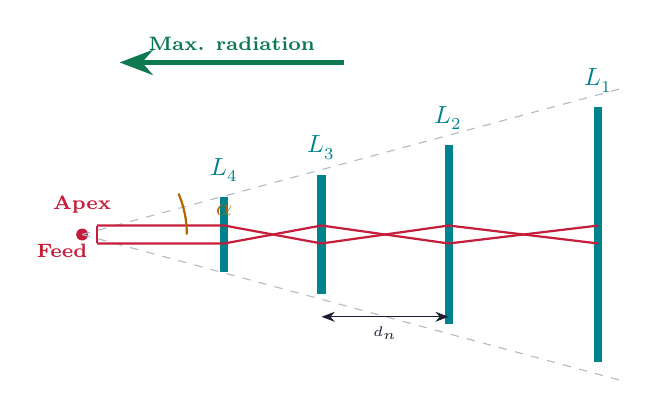
\begin{tikzpicture}[scale=0.95]
  % Apex
  \coordinate (A) at (-4, 0);
  \fill[myred] (A) circle (0.08);
  \node[above=4pt, font=\scriptsize\bfseries\color{myred}] at (-4, 0) {Apex};

  % Envelope lines (showing angular geometry)
  \draw[dashed, color=mgframe, thin] (A) -- (3.2, 1.95);
  \draw[dashed, color=mgframe, thin] (A) -- (3.2, -1.95);

  % Dipole elements (scaled geometrically, myteal)
  % L4 (smallest), L3, L2, L1 (largest)
  \foreach \x/\h/\lab in {-2.1/0.5/$L_4$, -0.8/0.8/$L_3$, 0.9/1.2/$L_2$, 2.9/1.7/$L_1$} {
    \draw[line width=3pt, color=myteal] (\x, -\h) -- (\x, \h);
    \node[above=2pt, font=\small\bfseries\color{myteal}] at (\x, \h) {\lab};
  }

  % Crossed (transposed) feed line — two wires swapping between elements
  \draw[thick, color=myred] (-3.8, 0.12) -- (-2.1, 0.12) -- (-0.8,-0.12) -- (0.9, 0.12) -- (2.9,-0.12);
  \draw[thick, color=myred] (-3.8,-0.12) -- (-2.1,-0.12) -- (-0.8, 0.12) -- (0.9,-0.12) -- (2.9, 0.12);

  % Feed connector at apex end
  \draw[thick, color=myred] (-3.8,-0.12) -- (-3.8, 0.12);
  \node[below left, font=\scriptsize\bfseries\color{myred}] at (-3.8, 0) {Feed};

  % Apex half-angle
  \draw[thick, color=myamber] (-2.6, 0) arc (0:23:1.4);
  \node[font=\small\bfseries\color{myamber}] at (-2.1, 0.32) {$\alpha$};

  % Spacing label d_n between L3 and L2
  \draw[Stealth-Stealth, thin, color=mydark] (-0.8,-1.1) -- (0.9,-1.1)
    node[midway, below, font=\tiny] {$d_n$};

  % Radiation direction (toward apex = left)
  \draw[-Stealth, line width=2pt, color=mygreen] (-0.5, 2.3) -- (-3.5, 2.3)
    node[midway, above, font=\scriptsize\bfseries\color{mygreen}] {Max. radiation};
\end{tikzpicture}
\end{tcolorbox}

\subsection{Principle of Operation (Active Region)}
The feed line is cross-phased between adjacent elements (a $180^\circ$ phase twist). This configuration ensures that at any given frequency:
\begin{itemize}[leftmargin=*, itemsep=3pt]
  \item \textbf{Transmission Region:} Elements that are too short ($L \ll \lambda/2$) present a high capacitive reactance and do not draw much current; they act as a transmission line.
  \item \textbf{Active Region:} Elements whose length is close to half a wavelength ($L \approx \lambda/2$) are resonant. They draw the majority of the current and radiate.
  \item \textbf{Reflective Region:} Elements that are too long ($L \gg \lambda/2$) are highly inductive and act as reflectors.
\end{itemize}
As the operating frequency increases, the active region shifts toward the smaller elements at the apex, maintaining constant beamwidth and input impedance.

% ===============================================================================
\section{Frequency Independent Antennas}
% ===============================================================================

\subsection{Rumsey's Principle}
Rumsey's Principle states that an antenna will be frequency-independent if its physical shape is defined entirely by angles, with no characteristic scale length. If the dimensions are scaled, the antenna looks identical except for a rotation.

\subsection{Examples}
\begin{itemize}[leftmargin=*, itemsep=3pt]
  \item \textbf{Biconical Antenna:} Formed by two co-axial metallic cones with their vertices facing each other. It behaves as a broadband version of a dipole.
  \item \textbf{Equiangular Spiral Antenna:} The boundary curves are defined in polar coordinates by:
  \[
  r = r_0 e^{a\phi}
  \]
  Because the shape is defined purely by exponential growth and angles, it has infinite theoretical bandwidth (practically limited by feed-point dimensions at high frequencies and outer boundaries at low frequencies).
\end{itemize}

\begin{tcolorbox}[tikzbox, title={Biconical Antenna Geometry}]
\centering
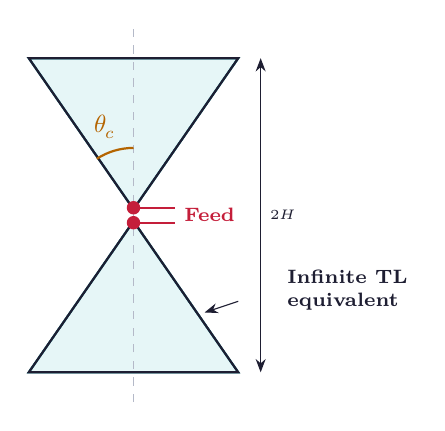
\begin{tikzpicture}[scale=0.95]
  % Top Cone
  \draw[thick, color=myteal, fill=hdrteal, fill opacity=0.7]
    (0,0.08) -- (-1.4,2.1) -- (1.4,2.1) -- cycle;
  % Bottom Cone
  \draw[thick, color=myteal, fill=hdrteal, fill opacity=0.7]
    (0,-0.08) -- (-1.4,-2.1) -- (1.4,-2.1) -- cycle;

  % Axis (dashed centre line)
  \draw[dashed, color=mgframe, thin] (0,-2.5) -- (0,2.5);

  % Cone edge outline for clarity
  \draw[thick, color=mydark] (0,0.08) -- (-1.4,2.1) -- (1.4,2.1) -- (0,0.08);
  \draw[thick, color=mydark] (0,-0.08) -- (-1.4,-2.1) -- (1.4,-2.1) -- (0,-0.08);

  % Half-angle arc and label
  \draw[thick, color=myamber] (0,0.9) arc (90:123:0.9);
  \node[font=\small\bfseries\color{myamber}] at (-0.38, 1.18) {$\theta_c$};

  % Feed gap
  \fill[myred] (0, 0.1) circle (0.09);
  \fill[myred] (0, -0.1) circle (0.09);
  \draw[thick, color=myred] (0,0.1) -- (0.55,0.1);
  \draw[thick, color=myred] (0,-0.1) -- (0.55,-0.1);
  \node[right, font=\scriptsize\bfseries\color{myred}] at (0.55, 0) {Feed};

  % Dimension: overall length
  \draw[Stealth-Stealth, thin, color=mydark] (1.7,-2.1) -- (1.7,2.1)
    node[midway, right, font=\tiny] {$2H$};

  % Label outside (right side, no overlap)
  \node[right=0.5cm, align=left, font=\scriptsize\color{mydark}] at (1.4, -1.0)
    {\textbf{Infinite TL}\\\textbf{equivalent}};
  \draw[-Stealth, thin, color=mydark] (1.4, -1.15) -- (0.95, -1.3);
\end{tikzpicture}
\end{tcolorbox}

% ===============================================================================
\section{Broadcast Antennas}
% ===============================================================================

Broadcast applications require omnidirectional radiation patterns in the horizontal plane to cover a $360^\circ$ service area.

\subsection{Turnstile Antenna}
A \textbf{turnstile antenna} consists of two identical horizontal half-wave dipoles placed perpendicular to each other ($90^\circ$ spatial separation) and excited with a $90^\circ$ phase difference.
\begin{itemize}[leftmargin=*, itemsep=2pt]
  \item The E-field components in the horizontal plane are:
  \[
  E_1 = E_0 \cos\phi, \quad E_2 = E_0 \sin\phi \, e^{j\pi/2} = j E_0 \sin\phi
  \]
  \item The total field is:
  \[
  E_{total} = E_1 + E_2 = E_0 (\cos\phi + j\sin\phi) = E_0 e^{j\phi}
  \]
  \item The magnitude $|E_{total}| = E_0$ is constant, producing a perfectly circular (omnidirectional) radiation pattern in the horizontal plane with circular polarization.
\end{itemize}

\subsection{Vertical Mast Radiators}
For Medium Frequency (MF) AM radio broadcasting, vertical steel towers (mast radiators) of height $H \approx \lambda/4$ or $H \approx 0.583\lambda$ (the anti-fading height, which minimizes sky-wave interference near the ground) are used. The ground acts as a reflector, forming a monopole equivalent.

\textbf{Radiation Pattern:} A vertical monopole of height $H$ over a perfectly conducting ground radiates an omnidirectional pattern in the azimuthal plane (horizontal). The elevation pattern $F(\theta)$ (measured from horizontal) is:
\[
F(\theta) = \frac{\cos(kH\sin\theta) - \cos(kH)}{\cos\theta}
\]
where $\theta$ is the elevation angle above the horizon. The pattern is maximum at $\theta = 0^\circ$ (horizontal, for ground-wave coverage) and zero at $\theta = 90^\circ$ (straight up).

\textbf{Why Anti-Fading Height ($H = 0.583\lambda$)?}
\begin{itemize}[leftmargin=*, itemsep=3pt]
  \item A $\lambda/4$ tower has its maximum radiation at the horizon and also radiates significantly at high angles, which creates strong sky waves. These sky waves reflect off the ionosphere and return as an interfering signal (fading).
  \item At $H = 0.583\lambda$, the pattern has a \textbf{null at the critical elevation angle} ($\approx 20^\circ$–$30^\circ$) from which ionospheric reflections would cause maximum interference in the primary service area. This suppresses the fading-causing sky wave while maintaining strong ground-wave coverage.
\end{itemize}

\textbf{Ground System:} A buried radial ground system (typically 120 radials of $\lambda/4$ length) is used to:
\begin{itemize}[leftmargin=*, itemsep=2pt]
  \item Provide a low-resistance current return path for the monopole image currents.
  \item Minimize ground losses and maximize radiation efficiency.
  \item Without a good ground system, $R_r$ is effectively in series with a high ground resistance, severely reducing efficiency.
\end{itemize}

\textbf{Effective Height ($h_e$):} The effective height of a monopole (a parameter used to calculate the open-circuit voltage induced in a receiving antenna) is:
\[
h_e = \frac{1}{I_0} \int_0^H I(z)\,dz
\]
For a $\lambda/4$ monopole with sinusoidal current: $h_e = \lambda/(2\pi) \approx 0.159\lambda$.

% ===============================================================================
% MANDATORY QUICK REVISION PAGE
% ===============================================================================
\newpage
\begin{center}
  {\large\bfseries\color{myred} Quick Revision --- Module 4}\\[3pt]
  {\small\color{mydark} Broadband and Broadcast Antennas $|$ PE-EC801A}
\end{center}
\noindent{\color{myred}\rule{\linewidth}{1.2pt}}
\vspace{4pt}

\begin{tcolorbox}[formulabox, title={\textbf{Key Formulas and Metrics at a Glance}}]
\renewcommand{\arraystretch}{1.35}
\begin{tabularx}{\linewidth}{B{5.2cm} X}
LPDA Scale Factor ($\tau$) & $\tau = \frac{L_{n+1}}{L_n} = \frac{R_{n+1}}{R_n} = \frac{d_{n+1}}{d_n} < 1$ \\[4pt]
LPDA Spacing Factor ($\sigma$) & $\sigma = \frac{d_n}{2 L_n}$ \\[4pt]
LPDA Apex Angle ($\alpha$) & $\tan\alpha = \frac{1 - \tau}{4 \sigma}$ \\[4pt]
Log-Spiral Geometry & $r = r_0 e^{a\phi}$ \quad (defined purely by angles) \\[4pt]
Yagi Driven Element Length & $L \approx 0.47\lambda$–$0.48\lambda$ \quad (usually folded dipole) \\[4pt]
Yagi Reflector Length & $L \approx 0.50\lambda$ \quad (inductive, reflects wave forward) \\[4pt]
Yagi Director Length & $L \approx 0.40\lambda$–$0.45\lambda$ \quad (capacitive, steers wave forward) \\
\end{tabularx}
\end{tcolorbox}

\begin{tcolorbox}[defbox, title={\textbf{One-Line Definitions}}]
\begin{itemize}[leftmargin=*, itemsep=2pt, topsep=0pt]
  \item \textbf{Parasitic Element:} An antenna element not electrically connected to the receiver/transmitter, excited via mutual coupling.
  \item \textbf{Folded Dipole:} A dipole antenna with its ends folded back and joined, providing a four-fold increase in input impedance.
  \item \textbf{Active Region:} The zone in a log-periodic array where elements are near resonance ($\approx \lambda/2$) and actively radiating.
  \item \textbf{Rumsey's Principle:} The condition that an antenna shape defined only by angles is frequency-independent.
  \item \textbf{Turnstile Antenna:} An arrangement of two crossed dipoles fed out of phase to produce a circular, omnidirectional horizontal pattern.
  \item \textbf{Anti-Fading Mast:} A vertical tower radiator of height $\approx 0.583\lambda$ that suppresses high-angle sky-wave radiation.
\end{itemize}
\end{tcolorbox}

\begin{tcolorbox}[exambox, title={\textbf{Frequently Asked / Viva Questions}}]
\begin{enumerate}[topsep=0pt, label=\textbf{Q\arabic*.}, itemsep=5pt]
  \item \Q{Explain the operation of parasitic elements in a Yagi-Uda antenna.}
    The reflector (longer than $\lambda/2$) acts inductively, shifting the phase of its re-radiated field to add constructively with the driven element's field in the forward direction. The directors (shorter than $\lambda/2$) act capacitively, shifting the phase to pull the beam forward.
  \item \Q{Why is a folded dipole used as the driven element in a Yagi-Uda antenna?}
    Adding parasitic elements near a dipole severely lowers its input impedance (often down to $<15\,\Omega$), causing mismatch loss. A folded dipole has a high impedance ($300\,\Omega$ in free space), which drops to a convenient $50$–$75\,\Omega$ in the array, making it easy to match to coaxial cables.
  \item \Q{What is the difference between a broadband antenna and a frequency-independent antenna?}
    A broadband antenna operates over a wide range (e.g., Yagi-Uda with $10\%$ bandwidth). A frequency-independent antenna satisfies Rumsey's principle (angular geometry) and has a practically unlimited bandwidth (often $10:1$ or more), as its active zone shifts continuously with frequency.
  \item \Q{How does a Log-Periodic Dipole Array (LPDA) achieve frequency independence?}
    As frequency changes, the "active region" (elements near $\lambda/2$ resonance) moves smoothly along the boom. The active elements scale geometrically, so the antenna's electrical size relative to the operating wavelength remains constant.
  \item \Q{What parameters define the geometry of an LPDA?}
    The geometric scale factor $\tau$ (ratio of adjacent lengths/spacings), the spacing factor $\sigma$ (ratio of spacing to element length), and the apex angle $\alpha$.
  \item \Q{How does a Turnstile antenna produce an omnidirectional pattern in the horizontal plane?}
    It uses two crossed horizontal dipoles fed in phase quadrature ($90^\circ$ phase shift). The resulting fields $E_0\cos\phi$ and $jE_0\sin\phi$ combine vectorially to yield a constant amplitude $|E| = E_0$ at all horizontal angles $\phi$.
  \item \Q{Why is the height of $0.583\lambda$ chosen for AM broadcast mast radiators?}
    At $0.583\lambda$, the antenna produces maximum ground-wave radiation while minimizing high-angle sky-wave radiation. This reduces interference between the ground wave and the ionospheric sky wave, preventing fading in the primary coverage zone.
\end{enumerate}
\end{tcolorbox}

\begin{tcolorbox}[tikzbox, title={Yagi-Uda vs. Log-Periodic Dipole Array (LPDA)}]
\centering
\renewcommand{\arraystretch}{1.55}
{\renewcommand{\arraystretch}{1.55}%
\begin{tabularx}{\linewidth}{|B{3.2cm}|Y|Y|}
\hline
\multicolumn{1}{|>{\centering\arraybackslash}m{3.2cm}|}{\textbf{Parameter}} &
\multicolumn{1}{>{\centering\arraybackslash}Y|}{\textbf{Yagi-Uda Antenna}} &
\multicolumn{1}{>{\centering\arraybackslash}Y|}{\textbf{Log-Periodic (LPDA)}} \\
\hline
Bandwidth & Narrow (typically $2\%$–$10\%$) & Extremely Wide ($10:1$ ratio or more) \\
\hline
Gain & High ($7$–$15\,\text{dB}$ depending on elements) & Moderate ($6$–$10\,\text{dB}$) \\
\hline
Element Design & Parasitic elements of specific lengths & Driven elements of geometrically scaled lengths \\
\hline
Feeder Connection & Driven element only (others mutually coupled) & All elements connected to a cross-phased line \\
\hline
\end{tabularx}}
\end{tcolorbox}


% -- Module 5 -----------------------------------------------------------------
\modulestart{5}{Characteristics of Microstrip Antennas}

\section{Characteristics of Microstrip Antennas}
% ===============================================================================

\begin{tcolorbox}[defbox, title={\textbf{Definition of Microstrip Patch Antenna}}]
A \textbf{microstrip patch antenna} consists of a radiating metallic patch (usually rectangular or circular) etched on one side of a thin, grounded dielectric substrate (dielectric constant $\epsilon_r$ and thickness $h$, where $h \ll \lambda$).
\end{tcolorbox}

\subsection{Physical Structure and Radiation Mechanism}
The metallic patch is usually made of copper or gold. The substrate thickness is typically $0.003\lambda_0 \le h \le 0.05\lambda_0$.
The patch acts as a resonant cavity with open-circuited edges. Fringing fields at the edges of the patch (along the length) act as the source of radiation. These fields extend slightly outside the physical boundaries, meaning the patch behaves electrically as if it were slightly larger than its physical dimensions.

\begin{tcolorbox}[tikzbox, title={Rectangular Microstrip Patch Antenna (Cross-Section and Top View)}]
\centering
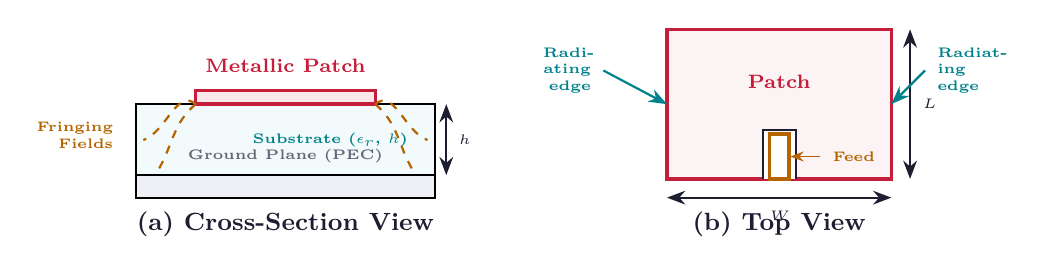
\begin{tikzpicture}[scale=0.95]
  % ── Cross-section view (left) ──────────────────────────────────────────────
  \begin{scope}[xshift=-3.8cm]
    % Ground plane — label above the bar so it doesn't clash with view title
    \draw[thick, fill=hdrgray] (-2.0,-1.25) rectangle (2.0,-0.95);
    \node[above=1pt, font=\tiny\bfseries\color{mydark}] at (0,-0.95) {Ground Plane (PEC)};
    % Substrate
    \draw[thick, fill=hdrteal, fill opacity=0.35] (-2.0,-0.95) rectangle (2.0,0.0);
    \node[font=\tiny\bfseries\color{myteal}] at (0.6,-0.48) {Substrate ($\epsilon_r$, $h$)};
    % Patch
    \draw[very thick, color=myred, fill=hdrred] (-1.2,0.0) rectangle (1.2,0.18);
    \node[above=3pt, font=\scriptsize\bfseries\color{myred}] at (0,0.18) {Metallic Patch};
    % Fringing fields — left edge only (symmetric), label well left
    \draw[thick, color=myamber, dashed] (-1.2, 0.0) to[out=140, in=20] (-1.9, -0.48);
    \draw[thick, color=myamber, dashed] (-1.2, 0.0) to[out=220, in=60] (-1.7, -0.88);
    \draw[thick, color=myamber, dashed] (1.2, 0.0) to[out=40, in=160] (1.9, -0.48);
    \draw[thick, color=myamber, dashed] (1.2, 0.0) to[out=-40, in=120] (1.7, -0.88);
    \node[left=2pt, align=right, font=\tiny\bfseries\color{myamber}] at (-2.1, -0.42) {Fringing\\Fields};
    % Height dimension — right side
    \draw[Stealth-Stealth, thick, color=mydark] (2.15,-0.95) -- (2.15, 0.0)
      node[midway, right=1pt, font=\tiny\bfseries] {$h$};
    % View label — placed well below with extra gap
    \node[font=\small\bfseries\color{mydark}] at (0,-1.6) {(a) Cross-Section View};
  \end{scope}

  % ── Top view (right) ───────────────────────────────────────────────────────
  \begin{scope}[xshift=2.8cm]
    % Patch rectangle
    \draw[very thick, color=myred, fill=hdrred, fill opacity=0.5]
      (-1.5,-1.0) rectangle (1.5,1.0);
    \node[font=\scriptsize\bfseries\color{myred}] at (0, 0.3) {Patch};
    % W dimension arrow — below patch, clear of feed line
    \draw[Stealth-Stealth, thick, color=mydark] (-1.5,-1.25) -- (1.5,-1.25)
      node[midway, below=1pt, font=\tiny\bfseries] {$W$};
    % L dimension arrow — right side
    \draw[Stealth-Stealth, thick, color=mydark] (1.75,-1.0) -- (1.75,1.0)
      node[midway, right=1pt, font=\tiny\bfseries] {$L$};
    % Inset notch in patch
    \fill[white] (-0.22,-1.0) rectangle (0.22,-0.35);
    \draw[thick, color=mydark] (-0.22,-1.0) -- (-0.22,-0.35)
      -- (0.22,-0.35) -- (0.22,-1.0);
    % Feed line — short, just below patch
    \draw[very thick, color=myamber] (-0.13,-1.0) rectangle (0.13,-0.4);
    % Feed line label — placed to the right with leader, NOT below W arrow
    \draw[-Stealth, thin, color=myamber] (0.55,-0.7) -- (0.15,-0.7);
    \node[right=1pt, font=\tiny\bfseries\color{myamber}] at (0.55,-0.7) {Feed};
    % Radiating edge labels — leader arrows pointing at edges
    \draw[Stealth-, thick, color=myteal] (-1.5, 0.0) -- (-2.35, 0.45);
    \node[left=1pt, align=right, text width=1.1cm, font=\tiny\bfseries\color{myteal}]
      at (-2.35, 0.45) {Radiating\\edge};
    \draw[Stealth-, thick, color=myteal] (1.5, 0.0) -- (1.95, 0.45);
    \node[right=1pt, align=left, text width=1.1cm, font=\tiny\bfseries\color{myteal}]
      at (1.95, 0.45) {Radiating\\edge};
    % View label
    \node[font=\small\bfseries\color{mydark}] at (0,-1.6) {(b) Top View};
  \end{scope}
\end{tikzpicture}
\end{tcolorbox}

\par\noindent
\textbf{Advantages and Disadvantages:}\par\noindent
{\renewcommand{\arraystretch}{1.45}%
\begin{tabularx}{\linewidth}{|Y|Y|}
\hline
\textbf{Advantages} & \textbf{Disadvantages} \\
\hline
Low profile, lightweight, conformable to surfaces. & Extremely narrow bandwidth (typically $1\%$–$5\%$). \\
\hline
Low fabrication cost (easy to print on PCBs). & Low radiation efficiency (due to dielectric and surface losses). \\
\hline
Supports dual-frequency and dual-polarization. & Low power handling capability. \\
\hline
\end{tabularx}}

% ===============================================================================
\section{Feeding Methods}
% ===============================================================================

To transfer electromagnetic energy into the patch, several feed techniques are used:

\begin{enumerate}[label=\textbf{\arabic*.}, leftmargin=*, itemsep=4pt]
  \item \textbf{Microstrip Line Feed:} A microstrip conducting strip feed is directly connected to the edge of the patch.
    \begin{itemize}[leftmargin=*, itemsep=1pt]
      \item \textit{Match method:} Inset cuts are made in the patch to match the high patch edge impedance to the feed line.
      \item \textit{Pros/Cons:} Easy to fabricate; but causes spurious feed radiation.
    \end{itemize}
  \item \textbf{Coaxial Probe Feed:} The outer conductor of a coaxial cable is connected to the ground plane, and the inner pin extends through the substrate and is soldered to the patch.
    \begin{itemize}[leftmargin=*, itemsep=1pt]
      \item \textit{Match method:} Match is achieved by choosing the insertion point offset from the patch edges.
      \item \textit{Pros/Cons:} Low spurious radiation; but requires drilling holes, making it harder to fabricate.
    \end{itemize}
  \item \textbf{Aperture-Coupled Feed:} The feed line is on a lower substrate, separated from the patch substrate by a common ground plane. Coupling occurs via a slot/aperture cut in the ground plane.
    \begin{itemize}[leftmargin=*, itemsep=1pt]
      \item \textit{Pros/Cons:} Shields feed line spurious radiation, improves bandwidth; but requires multilayer fabrication.
    \end{itemize}
  \item \textbf{Proximity-Coupled Feed:} The feed line is sandwiched between two substrate layers, and the patch is on the top surface. Energy couples electromagnetically.
    \begin{itemize}[leftmargin=*, itemsep=1pt]
      \item \textit{Pros/Cons:} Widest bandwidth (up to $13\%$), no contact needed; but complex to align.
    \end{itemize}
\end{enumerate}

\begin{tcolorbox}[tikzbox, title={Microstrip Line Feed vs. Coaxial Probe Feed}]
\centering
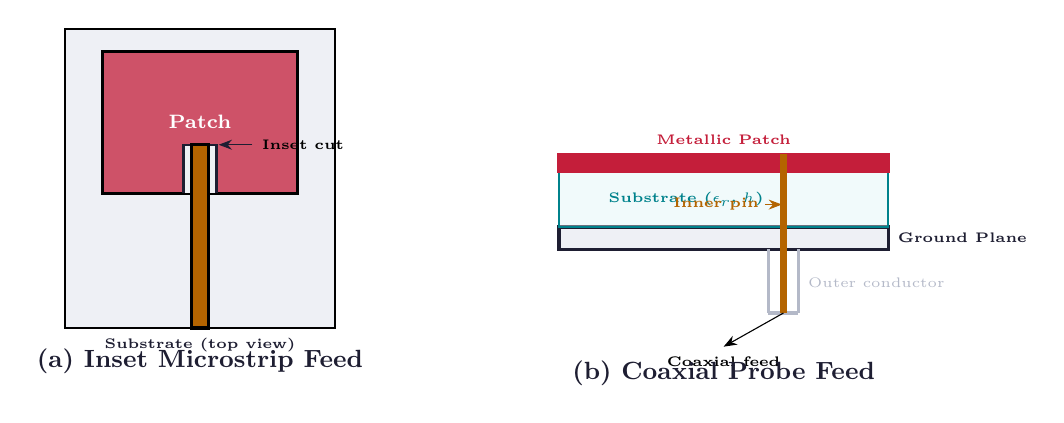
\begin{tikzpicture}[scale=0.95]
  % ── (a) Inset Microstrip Line Feed (top view) ──────────────────────────────
  \begin{scope}[xshift=-3.8cm]
    % Substrate / ground boundary shown as outer box
    \draw[thick, fill=hdrgray] (-1.8,-2.1) rectangle (1.8,1.9);
    \node[below, font=\tiny\bfseries\color{mydark}] at (0,-2.1) {Substrate (top view)};
    % Patch
    \draw[very thick, fill=myred, fill opacity=0.75] (-1.3,-0.3) rectangle (1.3,1.6);
    \node[font=\scriptsize\bfseries\color{white}] at (0, 0.65) {Patch};
    % Inset notch cut into patch
    \fill[hdrgray] (-0.22,-0.3) rectangle (0.22,0.35);
    \draw[thick, color=mydark] (-0.22,-0.3) -- (-0.22,0.35) -- (0.22,0.35) -- (0.22,-0.3);
    % Feed line (amber strip coming from bottom)
    \draw[very thick, fill=myamber] (-0.11,-2.1) rectangle (0.11,0.35);
    % Inset feed label
    \draw[-Stealth, thin, color=mydark] (0.7, 0.35) -- (0.25, 0.35);
    \node[right, font=\tiny\bfseries] at (0.7, 0.35) {Inset cut};
    % Dimension arrows
    \node[font=\tiny\bfseries\color{myamber}, below] at (0,-2.1) {};
    \node[font=\small\bfseries\color{mydark}] at (0,-2.55) {(a) Inset Microstrip Feed};
  \end{scope}

  % ── (b) Coaxial Probe Feed (cross-section view) ────────────────────────────
  \begin{scope}[xshift=3.2cm]
    % Ground plane (thick copper bar)
    \draw[very thick, fill=hdrgray, draw=mydark] (-2.2,-1.05) rectangle (2.2,-0.75);
    \node[right, font=\tiny\bfseries\color{mydark}] at (2.2,-0.9) {Ground Plane};
    % Substrate layer
    \draw[thick, fill=hdrteal, fill opacity=0.4, draw=myteal]
      (-2.2,-0.75) rectangle (2.2,0.0);
    \node[font=\tiny\bfseries\color{myteal}] at (-0.5,-0.38) {Substrate ($\epsilon_r$, $h$)};
    % Patch (top copper strip)
    \draw[very thick, fill=myred, draw=myred] (-2.2,0.0) rectangle (2.2,0.22);
    \node[above, font=\tiny\bfseries\color{myred}] at (0,0.22) {Metallic Patch};
    % Outer conductor of coax (below ground)
    \draw[very thick, color=mgframe] (0.6,-1.05) -- (0.6,-1.9);
    \draw[very thick, color=mgframe] (1.0,-1.05) -- (1.0,-1.9);
    \draw[very thick, color=mgframe] (0.6,-1.9) -- (1.0,-1.9);
    \node[right, font=\tiny\color{mgframe}] at (1.0,-1.5) {Outer conductor};
    % Inner pin (amber, goes through substrate to patch)
    \draw[line width=2.5pt, color=myamber] (0.8,-1.9) -- (0.8, 0.22);
    \node[left, font=\tiny\bfseries\color{myamber}] at (0.6,-0.45) {Inner pin};
    \draw[-Stealth, thin, color=myamber] (0.55,-0.45) -- (0.78,-0.45);
    % Coax label at bottom
    \draw[-Stealth, thin] (0.8,-1.9) -- (0.0,-2.35) node[below, font=\tiny\bfseries] {Coaxial feed};
    \node[font=\small\bfseries\color{mydark}] at (0,-2.7) {(b) Coaxial Probe Feed};
  \end{scope}
\end{tikzpicture}
\end{tcolorbox}

% ===============================================================================
\section{Methods of Analysis}
% ===============================================================================

\begin{itemize}[leftmargin=*, itemsep=3pt]
  \item \textbf{Transmission Line Model:} Simplest model. It represents the patch as a microstrip transmission line of length $L$ terminated by two radiating slots (modeled as parallel conductances $G$ and susceptances $B$). It yields good physical insight but is less accurate.
  \item \textbf{Cavity Model:} Represents the region between the patch and ground plane as a dielectric-loaded cavity with electric conductors on top/bottom, and artificial magnetic walls along the patch edges. It is more accurate and models higher-order modes.
  \item \textbf{Full-Wave Models:} Numerical techniques (such as the Method of Moments (MoM), Finite Element Method (FEM), or Finite Difference Time Domain (FDTD)). They are highly accurate for arbitrary shapes but are computationally demanding.
\end{itemize}

% ===============================================================================
\section{Design of Rectangular and Circular Patch Antennas}
% ===============================================================================

\subsection{Rectangular Patch Antenna Design}
The design parameters are: substrate height $h$, dielectric constant $\epsilon_r$, and resonant frequency $f_r$.

\begin{tcolorbox}[formulabox, title={\textbf{Rectangular Patch Design Calculations}}]
\begin{enumerate}[leftmargin=*, label=\textbf{\arabic*.}, itemsep=3pt, topsep=1pt]
  \item \textbf{Width ($W$):} To ensure high radiation efficiency, the width is:
  \[
  W = \frac{v_0}{2 f_r} \sqrt{\frac{2}{\epsilon_r + 1}}
  \]
  where $v_0 \approx 3 \times 10^8\,\text{m/s}$.
  \item \textbf{Effective Dielectric Constant ($\epsilon_{reff}$):} Accounts for fringing fields:
  \[
  \epsilon_{reff} = \frac{\epsilon_r + 1}{2} + \frac{\epsilon_r - 1}{2} \left[ 1 + 12 \frac{h}{W} \right]^{\!-1/2}
  \]
  \item \textbf{Extended Patch Length ($\Delta L$):} Due to fringing fields:
  \[
  \Delta L = 0.412 h \frac{(\epsilon_{reff} + 0.3)\left(\frac{W}{h} + 0.264\right)}{(\epsilon_{reff} - 0.258)\left(\frac{W}{h} + 0.8\right)}
  \]
  \item \textbf{Physical Length ($L$):}
  \[
  L = L_{eff} - 2\Delta L = \frac{v_0}{2 f_r \sqrt{\epsilon_{reff}}} - 2\Delta L
  \]
\end{enumerate}
\end{tcolorbox}

\begin{tcolorbox}[examplebox, title={\textbf{Worked Example: Rectangular Patch at 2.4 GHz}}]
\textbf{Given:} $f_r = 2.4\,\text{GHz}$, FR-4 substrate: $\epsilon_r = 4.4$, $h = 1.6\,\text{mm}$.

\textbf{Step 1 — Width:}
\[
W = \frac{3 \times 10^8}{2 \times 2.4 \times 10^9}\sqrt{\frac{2}{4.4+1}} = 0.0625 \times 0.609 \approx 38.0\,\text{mm}
\]

\textbf{Step 2 — Effective dielectric constant:}
\[
\epsilon_{reff} = \frac{4.4+1}{2} + \frac{4.4-1}{2}\left[1 + 12\frac{1.6}{38.0}\right]^{-1/2} = 2.7 + 1.7 \times 0.857 \approx 4.16
\]

\textbf{Step 3 — Extension:}
\[
\Delta L = 0.412 \times 1.6 \times \frac{(4.16+0.3)(38.0/1.6+0.264)}{(4.16-0.258)(38.0/1.6+0.8)} \approx 0.749\,\text{mm}
\]

\textbf{Step 4 — Physical length:}
\[
L = \frac{3\times10^8}{2 \times 2.4\times10^9 \times \sqrt{4.16}} - 2 \times 0.749 = 30.7 - 1.5 \approx 29.2\,\text{mm}
\]

\textbf{Result:} $W \approx 38\,\text{mm}$, $L \approx 29.2\,\text{mm}$ on a $1.6\,\text{mm}$ FR-4 substrate.
\end{tcolorbox}

\subsection{Circular Patch Antenna Design}
For a circular patch of radius $a$ on a substrate of height $h$, the dominant resonant mode is $TM^z_{110}$.

\subsubsection*{Resonant Modes and Radiation Mechanism}
The circular patch behaves as a \textbf{resonant cavity} bounded by:
\begin{itemize}[leftmargin=*, itemsep=2pt]
  \item \textbf{Top and bottom:} Perfect Electric Conductor (PEC) walls — the patch and ground plane.
  \item \textbf{Side boundary:} Perfect Magnetic Conductor (PMC) wall (fringing field approximation).
\end{itemize}
The resonant modes are designated $TM^z_{nmp}$ where:
\begin{itemize}[leftmargin=*, itemsep=2pt]
  \item $n$ = number of full-period variations in $\phi$ (azimuthal direction)
  \item $m$ = number of zeros of $J_n'(\cdot)$ in the radial direction ($m = 1, 2, 3, \dots$)
  \item $p$ = number of variations in $z$ (always $0$ for thin patches since $h \ll \lambda$)
\end{itemize}

The \textbf{dominant mode} $TM^z_{110}$ has:
\begin{itemize}[leftmargin=*, itemsep=2pt]
  \item One full-period azimuthal variation ($n=1$) and the first radial maximum ($m=1$).
  \item The constant $1.8412$ is the first root of $J_1'(\chi_{11}) = 0$ (derivative of first-order Bessel function), which defines the resonance condition.
  \item \textbf{Broadside radiation pattern} — maximum gain perpendicular to the patch surface ($\theta = 0^\circ$).
  \item \textbf{Linear polarization} — the $E$-field across the radiating edge is linearly polarized.
\end{itemize}

\subsubsection*{Higher-Order Modes}
Other useful modes include:
\begin{itemize}[leftmargin=*, itemsep=3pt]
  \item $TM^z_{010}$: Omnidirectional (monopole-like) radiation; used for low-profile omnidirectional antennas.
  \item $TM^z_{210}$: Figure-8 pattern; used for circular polarization when combined with $TM^z_{110}$.
  \item \textbf{Dual-Band Operation:} By stacking two circular patches of different radii on separate substrate layers, two resonant frequencies can be achieved independently.
\end{itemize}

\subsubsection*{Circular Polarization from a Circular Patch}
Circular polarization (CP) is an important feature achievable with circular patches:
\begin{itemize}[leftmargin=*, itemsep=3pt]
  \item \textbf{Single feed CP:} A slight perturbation (small notch or truncation of the circular boundary) splits the degenerate $TM^z_{110}$ mode into two orthogonal modes with a $90^\circ$ phase separation. CP results when the two modes are excited with equal amplitude and $90^\circ$ phase shift.
  \item \textbf{Two-feed CP:} Two coaxial probes placed at $90^\circ$ apart on the patch perimeter, fed with equal amplitude and a $90^\circ$ hybrid coupler, produce clean CP over a wider bandwidth.
\end{itemize}

\subsubsection*{Fringing Fields and Effective Radius}
The fringing fields at the patch edge extend the effective electrical radius beyond the physical radius:
\[
a_e = a + \Delta a \quad \text{where} \quad \Delta a = a\left[\sqrt{1 + \frac{2h}{\pi\epsilon_r a}\left(\ln\frac{\pi a}{2h} + 1.7726\right)} - 1\right]
\]
Typically $\Delta a / a \approx 1\%$–$5\%$ for standard substrates. A higher $\epsilon_r$ or thinner substrate reduces the fringing correction.

\subsubsection*{Substrate Selection Tradeoffs}

\par\noindent
{\renewcommand{\arraystretch}{1.55}
\begin{tabularx}{\linewidth}{|B{3.0cm}|Y|Y|}
\hline
\textbf{Parameter} & \textbf{High $\epsilon_r$ (e.g., 10)} & \textbf{Low $\epsilon_r$ (e.g., 2.2)} \\
\hline
Patch Size & Smaller (compact) & Larger \\
\hline
Bandwidth & Narrower & Wider \\
\hline
Radiation Efficiency & Lower (more stored energy) & Higher \\
\hline
Surface Wave Loss & Higher & Lower \\
\hline
Typical Use & Miniaturised antenna-on-chip & High-performance arrays \\
\hline
\end{tabularx}}

\textbf{Design Procedure:}
\begin{enumerate}[label=\textbf{\arabic*.}, leftmargin=*, itemsep=3pt]
  \item Specify desired resonant frequency $f_r$, substrate $\epsilon_r$ and thickness $h$.
  \item Compute intermediate parameter $F$ (an estimate of the effective radius assuming no fringing).
  \item Solve for physical radius $a$ by applying the fringing correction factor.
  \item Compute effective radius $a_e$.
  \item Verify by back-calculating $(f_r)_{110}$ — should match the target within $1\%$.
  \item Choose feed position (coaxial probe offset from centre) to match $50\,\Omega$.
\end{enumerate}

\textbf{Typical example:} Circular patch at $f_r = 2.4\,\text{GHz}$, FR-4 substrate ($\epsilon_r = 4.4$, $h = 1.6\,\text{mm}$):
$F \approx 17.5\,\text{mm}$, $a \approx 16.8\,\text{mm}$, $a_e \approx 17.2\,\text{mm}$.
Bandwidth $\approx 1\%$–$3\%$, directivity $\approx 6$–$7\,\text{dBi}$.

\subsubsection*{Comparison: Circular vs. Rectangular Patch}

\par\noindent
{\renewcommand{\arraystretch}{1.55}
\begin{tabularx}{\linewidth}{|B{3.2cm}|Y|Y|}
\hline
\textbf{Property} & \textbf{Rectangular Patch} & \textbf{Circular Patch} \\
\hline
Shape & Rectangular ($W \times L$) & Circular (radius $a$) \\
\hline
Resonant parameter & Length $L \approx \lambda/(2\sqrt{\epsilon_{reff}})$ & Radius $a$ from Bessel zero \\
\hline
Dominant mode & $TM^x_{100}$ & $TM^z_{110}$ \\
\hline
Bandwidth & $\approx 1\%$–$5\%$ & $\approx 1\%$–$3\%$ (slightly narrower) \\
\hline
Circular Polarization & Possible with square patch + notch & Easier — natural symmetry aids CP \\
\hline
Compactness & Larger footprint & More compact (round shape) \\
\hline
Design Complexity & Simpler formulas & Slightly more involved (Bessel functions) \\
\hline
\end{tabularx}}

\begin{tcolorbox}[formulabox, title={\textbf{Circular Patch Design Equations}}]
The physical radius $a$ is calculated as:
\[
a = \frac{F}{\left\{ 1 + \frac{2h}{\pi \epsilon_r F} \left[ \ln\left(\frac{\pi F}{2h}\right) + 1.7726 \right] \right\}^{1/2}}
\]
where:
\[
F = \frac{8.791 \times 10^9}{f_r \sqrt{\epsilon_r}} \quad (\text{for } f_r \text{ in Hz})
\]
The effective radius $a_e$ incorporating fringing fields is:
\[
a_e = a \left\{ 1 + \frac{2h}{\pi \epsilon_r a} \left[ \ln\left(\frac{\pi a}{2h}\right) + 1.7726 \right] \right\}^{1/2}
\]
The resonant frequency for the $TM^z_{110}$ mode is:
\[
(f_r)_{110} = \frac{1.8412 v_0}{2\pi a_e \sqrt{\epsilon_r}}
\]
\end{tcolorbox}

% ===============================================================================
% MANDATORY QUICK REVISION PAGE
% ===============================================================================
\newpage
\begin{center}
  {\large\bfseries\color{myred} Quick Revision --- Module 5}\\[3pt]
  {\small\color{mydark} Microstrip Antennas $|$ PE-EC801A}
\end{center}
\noindent{\color{myred}\rule{\linewidth}{1.2pt}}
\vspace{4pt}

\begin{tcolorbox}[formulabox, title={\textbf{Key Formulas and Metrics at a Glance}}]
\renewcommand{\arraystretch}{1.35}
\begin{tabularx}{\linewidth}{B{5.2cm} X}
Rectangular Patch Width ($W$) & $W = \frac{v_0}{2 f_r} \sqrt{\frac{2}{\epsilon_r + 1}}$ \\[4pt]
Effective Dielectric ($\epsilon_{reff}$) & $\epsilon_{reff} = \frac{\epsilon_r + 1}{2} + \frac{\epsilon_r - 1}{2} \left[ 1 + 12 \frac{h}{W} \right]^{-1/2}$ \\[4pt]
Extended Length ($\Delta L$) & $\Delta L \approx 0.412 h \frac{(\epsilon_{reff} + 0.3)(W/h + 0.264)}{(\epsilon_{reff} - 0.258)(W/h + 0.8)}$ \\[4pt]
Physical Length ($L$) & $L = \frac{v_0}{2 f_r \sqrt{\epsilon_{reff}}} - 2\Delta L$ \\[4pt]
Resonant circular frequency & $(f_r)_{110} = \frac{1.8412 v_0}{2\pi a_e \sqrt{\epsilon_r}}$ \\[4pt]
Effective circular radius ($a_e$) & $a_e = a \left\{ 1 + \frac{2h}{\pi \epsilon_r a} \left[ \ln\left(\frac{\pi a}{2h}\right) + 1.7726 \right] \right\}^{1/2}$ \\
\end{tabularx}
\end{tcolorbox}

\begin{tcolorbox}[defbox, title={\textbf{One-Line Definitions}}]
\begin{itemize}[leftmargin=*, itemsep=2pt, topsep=0pt]
  \item \textbf{Fringing Fields:} The bending of electric field lines at the open-circuit boundaries of a microstrip patch, which enables radiation.
  \item \textbf{Inset Feed:} A feed technique where notch cuts are made in the patch to match the low line impedance ($\approx 50\,\Omega$) directly inside the patch.
  \item \textbf{Transmission Line Model:} An analytical model that treats a rectangular patch antenna as two radiating slots separated by a transmission line.
  \item \textbf{Cavity Model:} An analysis model that treats the patch as a cavity bounded by perfect electric and magnetic walls.
  \item \textbf{Full-Wave Analysis:} Direct numerical solvers of Maxwell's equations (e.g., FEM, FDTD) used for complex microstrip geometries.
\end{itemize}
\end{tcolorbox}

\begin{tcolorbox}[exambox, title={\textbf{Frequently Asked / Viva Questions}}]
\begin{enumerate}[topsep=0pt, label=\textbf{Q\arabic*.}, itemsep=5pt]
  \item \Q{What is the primary mechanism of radiation in microstrip patch antennas?}
    Radiation is generated by the fringing fields at the patch edges. These fringing fields act as slot sources along the radiating edges (separated by $L \approx \lambda/2$).
  \item \Q{Compare microstrip line feeding and coaxial probe feeding.}
    Microstrip line feeds are simple to fabricate but introduce spurious radiation from the feed line, which degrades the radiation pattern. Coaxial probe feeding offers lower spurious radiation and easy matching, but requires drilling holes, making fabrication more complex.
  \item \Q{What is the purpose of an inset feed in microstrip antennas?}
    The input impedance at the edge of a patch is high (typically $200$–$300\,\Omega$). An inset notch shifts the contact point of the feed line toward the center of the patch, where the impedance is lower, matching it to a standard $50\,\Omega$ transmission line.
  \item \Q{Why does a microstrip patch antenna have a narrow bandwidth?}
    The patch antenna behaves electrically as a high-Q resonant cavity with a small volume. Since the substrate height $h$ is thin ($h \ll \lambda$), the energy stored in the cavity is high compared to the energy radiated, leading to a narrow bandwidth.
  \item \Q{Explain the physical meaning of the effective dielectric constant ($\epsilon_{reff}$).}
    Because the fringing field lines travel partly through the dielectric substrate and partly through the surrounding air, the wave behaves as if it were propagating through a homogeneous medium with a dielectric constant $\epsilon_{reff}$ that lies between $1$ (air) and $\epsilon_r$ (substrate).
  \item \Q{State the advantages of aperture-coupled feeds over direct feeding methods.}
    The ground plane separates the feed line from the radiating patch, preventing spurious feed line radiation from distorting the antenna's far-field radiation pattern. It also allows independent optimization of the feed and patch substrate thicknesses.
\end{enumerate}
\end{tcolorbox}

\begin{tcolorbox}[tikzbox, title={Comparison of Patch Feeding Methods}]
\centering
\renewcommand{\arraystretch}{1.55}
{\renewcommand{\arraystretch}{1.55}%
\begin{tabularx}{\linewidth}{|B{3.2cm}|Y|Y|Y|}
\hline
\multicolumn{1}{|>{\centering\arraybackslash}m{3.2cm}|}{\textbf{Feed Type}} &
\multicolumn{1}{>{\centering\arraybackslash}Y|}{\textbf{Ease of Fab}} &
\textbf{Spurious Radiation} &
\textbf{Relative Bandwidth} \\
\hline
Microstrip Line & Very Easy & High & Narrow ($1$–$2\%$) \\
\hline
Coaxial Probe & Moderate (requires drilling) & Low & Narrow ($1$–$3\%$) \\
\hline
Aperture Coupled & Complex (multilayer alignment) & Lowest (shielded by ground) & Moderate ($4$–$5\%$) \\
\hline
Proximity Coupled & Complex (multilayer alignment) & Low & Widest ($10$–$13\%$) \\
\hline
\end{tabularx}}
\end{tcolorbox}


% -- Module 6 -----------------------------------------------------------------
\modulestart{6}{Uniform Linear Arrays (ULA)}

\section{Uniform Linear Arrays (ULA)}
% ===============================================================================

\begin{tcolorbox}[defbox, title={\textbf{Definition of an Antenna Array}}]
An \textbf{antenna array} is a set of two or more identical antenna elements positioned and excited such that their individual radiation fields combine constructively in desired directions and cancel destructively in other directions, increasing directivity.
\end{tcolorbox}

\subsection{Two-Element Array Analysis}
Consider two identical antennas separated by a distance $d$ along the $z$-axis. Antenna 1 is at the origin and serves as the phase reference ($I_1 = I_0 e^{j0}$). Antenna 2 is fed with a phase lead $\beta$ ($I_2 = I_0 e^{j\beta}$).

\begin{tcolorbox}[tikzbox, title={Two-Element Array Geometry}]
\centering
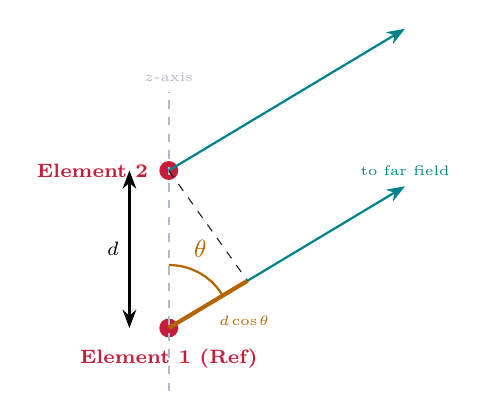
\begin{tikzpicture}[scale=1.0]
  % Antennas
  \fill[myred] (0,0) circle (0.12) node[below=4pt, font=\scriptsize\bfseries] {Element 1 (Ref)};
  \fill[myred] (0,2.0) circle (0.12) node[left=4pt, font=\scriptsize\bfseries] {Element 2};

  % Array axis
  \draw[dashed, thick, color=mgframe] (0,-0.8) -- (0,3.0) node[above, font=\tiny] {$z$-axis};

  % Rays to far field
  \draw[-Stealth, thick, color=myteal] (0,0) -- (3.0,1.8) node[above, font=\tiny] {to far field};
  \draw[-Stealth, thick, color=myteal] (0,2.0) -- (3.0,3.8);

  % Perpendicular for path difference
  \draw[dashed, color=mydark] (0,2.0) -- (1.0, 0.6);
  \draw[line width=1.5pt, color=myamber] (0,0) -- (1.0,0.6) node[midway, below right, font=\tiny\bfseries] {$d\cos\theta$};

  % Angle
  \draw[thick, color=myamber] (0,0.8) arc (90:31:0.8);
  \node[color=myamber, font=\small\bfseries] at (0.4, 1.0) {$\theta$};

  % Spacing
  \draw[Stealth-Stealth, thick] (-0.5,0) -- (-0.5,2.0) node[midway, left, font=\scriptsize] {$d$};

\end{tikzpicture}
\end{tcolorbox}

In the far field, the path difference between the waves is $d\cos\theta$ (where $\theta$ is measured from the array axis). The total phase difference $\psi$ between the fields is:
\[
\psi = kd\cos\theta + \beta
\]
The total far-field electric field is:
\[
E_{total} = E_1 + E_2 = E_0 \left( 1 + e^{j(kd\cos\theta + \beta)} \right) = E_0 e^{j\psi/2} \left( 2\cos\frac{\psi}{2} \right)
\]
The normalized \textbf{Array Factor (AF)} is:
\[
AF_n(\theta) = \cos\left( \frac{kd\cos\theta + \beta}{2} \right)
\]

\subsection{N-Element Uniform Linear Array (ULA)}
For $N$ identical elements fed with equal amplitude $I_0$ and progressive phase shift $\beta$:
\[
AF = \sum_{n=0}^{N-1} e^{j n (kd\cos\theta + \beta)} = \sum_{n=0}^{N-1} e^{j n \psi}
\]
Summing this geometric progression:
\[
|AF| = \left| \frac{\sin\left(\frac{N}{2}\psi\right)}{\sin\left(\frac{1}{2}\psi\right)} \right| \implies |AF_n| = \left| \frac{\sin\left(\frac{N}{2}(kd\cos\theta + \beta)\right)}{N \sin\left(\frac{1}{2}(kd\cos\theta + \beta)\right)} \right|
\]

\subsection{Broadside vs. End-Fire Arrays}
\begin{enumerate}[label=\textbf{\arabic*.}, leftmargin=*, itemsep=4pt]
  \item \textbf{Broadside Array:} Maximum radiation is perpendicular to the array axis ($\theta = 90^\circ$).
    \begin{itemize}[leftmargin=*, itemsep=1pt]
      \item \textit{Condition:} $\psi = 0$ at $\theta = 90^\circ \implies kd\cos(90^\circ) + \beta = 0 \implies \beta = 0$.
      \item \textit{Nulls:} Occur when $\sin(N\psi/2) = 0 \implies \theta_{null} = \cos^{-1}\left( \pm \frac{m\lambda}{Nd} \right), \quad m = 1, 2, 3, \dots$
    \end{itemize}
  \item \textbf{End-Fire Array:} Maximum radiation is along the array axis ($\theta = 0^\circ$ or $180^\circ$).
    \begin{itemize}[leftmargin=*, itemsep=1pt]
      \item \textit{Condition for $\theta = 0^\circ$:} $\psi = 0 \implies kd\cos(0^\circ) + \beta = 0 \implies \beta = -kd$.
      \item \textit{Condition for $\theta = 180^\circ$:} $\psi = 0 \implies kd\cos(180^\circ) + \beta = 0 \implies \beta = kd$.
    \end{itemize}
\end{enumerate}

\subsection{Key ULA Performance Formulas}
For a uniform linear array of $N$ elements with spacing $d$:
\begin{itemize}[leftmargin=*, itemsep=3pt]
  \item \textbf{Broadside HPBW:}
  \[
  \text{HPBW} \approx \frac{0.886\,\lambda}{N d} \text{ rad} = \frac{50.8^\circ \lambda}{Nd}
  \]
  The beamwidth narrows as $N$ or $d$ increases — doubling the array length halves the HPBW.
  \item \textbf{Broadside Directivity:}
  \[
  D \approx \frac{2Nd}{\lambda} \quad \text{(for } d \le \lambda/2 \text{)}
  \]
  \item \textbf{End-Fire HPBW:}
  \[
  \text{HPBW} \approx 2\sqrt{\frac{2\lambda}{Nd}} \text{ rad}
  \]
  \item \textbf{First Sidelobe Level (Uniform Excitation):} $-13.5\,\text{dB}$ below the main beam — independent of $N$.
\end{itemize}

% ===============================================================================
\section{Non-Uniform Amplitude Arrays}
% ===============================================================================

Uniform arrays have high directivity but suffer from relatively high sidelobes ($-13.5\,\text{dB}$ for the first sidelobe). To reduce sidelobes, elements can be excited with non-uniform current amplitudes.

\subsection{Binomial Array}
The excitation amplitudes of the elements correspond to the coefficients of a binomial expansion:
\[
a_n = \binom{N-1}{n}, \quad n = 0, 1, \dots, N-1
\]
For example, for a 5-element array, the amplitudes scale as $1 : 4 : 6 : 4 : 1$.
\begin{itemize}[leftmargin=*, itemsep=2pt]
  \item \textbf{Advantage:} Completely eliminates sidelobes if the element spacing $d \le \lambda/2$.
  \item \textbf{Disadvantage:} Broader beamwidth (HPBW) and lower directivity than a uniform array of equivalent length.
\end{itemize}

\subsection{Dolph-Tschebyscheff Array}
This array uses Tschebyscheff (Chebyshev) polynomials $T_m(z)$ to design a pattern with a specified sidelobe level (SLL) and the narrowest possible main beamwidth.
The Chebyshev polynomials are defined by:
\[
T_m(z) = \cos(m \cos^{-1} z) \quad (|z| \le 1)
\]
\[
T_m(z) = \cosh(m \cosh^{-1} z) \quad (|z| > 1)
\]
This method optimizes the trade-off by ensuring that all sidelobes are at the exact same specified level (e.g., $-20\,\text{dB}$ or $-30\,\text{dB}$).

\textbf{Design Procedure:}
\begin{enumerate}[label=\textbf{\arabic*.}, leftmargin=*, itemsep=3pt]
  \item Specify the number of elements $N$ (array order $m = N-1$) and the desired sidelobe level ratio $R$ (e.g., $R = 26.3$ for $-20\,\text{dB}$ SLL; $R = 10^{SLL_{dB}/20}$).
  \item Compute the parameter $z_0$ that maps the main lobe maximum to $T_m(z_0)$:
  \[
  z_0 = \cosh\!\left[ \frac{1}{m} \cosh^{-1}(R) \right]
  \]
  \item Substitute $z = z_0 \cos\!\left(\frac{\psi}{2}\right)$ into $T_m(z)$ to obtain the array polynomial. The AF takes the form $AF(\psi) = T_m\!\left(z_0 \cos\frac{\psi}{2}\right)$.
  \item Extract the excitation coefficients $a_n$ by expanding the Chebyshev polynomial in powers of $\cos^n\!\left(\frac{\psi}{2}\right)$.
\end{enumerate}

\textbf{Key result:} For a 5-element array with $-20\,\text{dB}$ SLL, the excitation amplitudes are approximately $1 : 2.41 : 3.14 : 2.41 : 1$ (compare to binomial $1:4:6:4:1$ — Dolph gives a narrower beam for the same SLL).

% ===============================================================================
\section{Extension to Planar Arrays}
% ===============================================================================

A \textbf{planar array} consists of elements positioned in a two-dimensional grid (e.g., $M$ elements along $x$ with spacing $d_x$, and $N$ elements along $y$ with spacing $d_y$).

The overall Array Factor is the product of the individual linear array factors along the two directions:
\[
AF_{planar} = AF_x \cdot AF_y = \left[ \frac{\sin\left(\frac{M}{2}\psi_x\right)}{\sin\left(\frac{1}{2}\psi_x\right)} \right] \left[ \frac{\sin\left(\frac{N}{2}\psi_y\right)}{\sin\left(\frac{1}{2}\psi_y\right)} \right]
\]
where:
\[
\psi_x = k d_x \sin\theta \cos\phi + \beta_x
\]
\[
\psi_y = k d_y \sin\theta \sin\phi + \beta_y
\]
By dynamically adjusting the phase shifters $\beta_x$ and $\beta_y$, the main beam can be steered to any coordinate ($\theta_0, \phi_0$) in 3D space:
\[
\beta_x = -k d_x \sin\theta_0 \cos\phi_0
\]
\[
\beta_y = -k d_y \sin\theta_0 \sin\phi_0
\]

% ===============================================================================
\section{Antenna Array Synthesis}
% ===============================================================================

Array synthesis involves finding the feeding currents (amplitudes and phases) and element locations required to produce a desired radiation pattern.

\subsection{Schelkunoff Polynomial Method}
Schelkunoff represented the array factor of an $N$-element linear array as a polynomial in the complex variable $z = e^{j\psi}$:
\[
AF = \sum_{n=0}^{N-1} a_n z^n = a_{N-1} (z - z_1)(z - z_2) \dots (z - z_{N-1})
\]
where $z_i$ are the roots (zeros) of the polynomial. Since $z$ lies on the unit circle ($|z| = 1$), the nulls in the radiation pattern correspond to the roots that lie on the unit circle.

\textbf{Visible Region:} As $\theta$ varies from $0^\circ$ to $180^\circ$, $\psi = kd\cos\theta + \beta$ traces an arc on the unit circle in the complex $z$-plane. This arc is called the \textbf{visible region}:
\[
-kd + \beta \le \psi \le kd + \beta
\]
\begin{itemize}[leftmargin=*, itemsep=3pt]
  \item For $d = \lambda/2$ and $\beta = 0$: visible region spans $-\pi \le \psi \le \pi$ (full circle).
  \item For $d < \lambda/2$: visible region is less than a full circle — some roots in the \textbf{invisible region} do not contribute to the radiation pattern.
  \item Placing a root \textit{inside} the visible region creates a null in the pattern. Placing a root \textit{outside} the visible region eliminates that null.
\end{itemize}
This allows designers to synthesize specific patterns by precisely controlling which roots lie on vs. off the visible arc.

\subsection{Woodward-Lawson Method}
The Woodward-Lawson method synthesizes a desired source pattern by superimposing several independent, orthogonal beams (each having a $\frac{\sin(N\psi/2)}{N\sin(\psi/2)}$ shape centred at different angles). The excitation coefficients are found by sampling the desired pattern at the beam centres.

\textbf{Sampling formula:} For $N$ elements, the array factor is:
\[
AF(\psi) = \sum_{m=-(N-1)/2}^{(N-1)/2} c_m \cdot \frac{\sin\!\left[\frac{N}{2}(\psi - \psi_m)\right]}{N\sin\!\left[\frac{1}{2}(\psi - \psi_m)\right]}
\]
where each beam is centred at $\psi_m = \frac{2\pi m}{N}$ and the sampling coefficients $c_m$ are found by evaluating the desired pattern $F_d(\psi)$ at those points:
\[
c_m = F_d(\psi_m) = F_d\!\left(\frac{2\pi m}{N}\right)
\]

\textbf{Key properties:}
\begin{itemize}[leftmargin=*, itemsep=2pt]
  \item The synthesized pattern passes exactly through the desired sample values.
  \item Between sample points, the approximation may deviate (Gibbs-like ripple for abrupt transitions).
  \item Adding more elements $N$ increases the number of sample points and improves accuracy.
  \item Suitable for pencil-beam, sector, flat-top, or shaped beam synthesis.
\end{itemize}

% ===============================================================================
% MANDATORY QUICK REVISION PAGE
% ===============================================================================
\newpage
\begin{center}
  {\large\bfseries\color{myred} Quick Revision --- Module 6}\\[3pt]
  {\small\color{mydark} Antenna Arrays and Synthesis $|$ PE-EC801A}
\end{center}
\noindent{\color{myred}\rule{\linewidth}{1.2pt}}
\vspace{4pt}

\begin{tcolorbox}[formulabox, title={\textbf{Key Formulas and Metrics at a Glance}}]
\renewcommand{\arraystretch}{1.35}
\begin{tabularx}{\linewidth}{B{5.2cm} X}
N-Element ULA Array Factor ($AF$) & $AF = \frac{\sin(N\psi/2)}{\sin(\psi/2)}$ \quad where $\psi = kd\cos\theta + \beta$ \\[4pt]
Broadside Phase Shift ($\beta$) & $\beta = 0$ \\[4pt]
End-Fire Phase Shift ($\beta$) & $\beta = \mp kd$ \quad (for $\theta = 0^\circ$ or $180^\circ$ main beam) \\[4pt]
Broadside HPBW & $\text{HPBW} \approx \frac{0.886\lambda}{Nd}$ rad $\approx \frac{50.8^\circ\lambda}{Nd}$ \\[4pt]
Broadside Directivity & $D \approx \frac{2Nd}{\lambda}$ \quad (uniform excitation, $d \le \lambda/2$) \\[4pt]
Binomial Array Coefficients & $a_n = \binom{N-1}{n} = \frac{(N-1)!}{n!(N-1-n)!}$ \\[4pt]
Planar Beam Steering Phase & $\beta_x = -k d_x \sin\theta_0 \cos\phi_0, \quad \beta_y = -k d_y \sin\theta_0 \sin\phi_0$ \\[4pt]
Schelkunoff Complex Variable ($z$) & $z = e^{j\psi} = e^{j(kd\cos\theta + \beta)}$ \\
\end{tabularx}
\end{tcolorbox}

\begin{tcolorbox}[defbox, title={\textbf{One-Line Definitions}}]
\begin{itemize}[leftmargin=*, itemsep=2pt, topsep=0pt]
  \item \textbf{Array Factor:} The radiation pattern of an array of isotropic elements, describing how the geometry and feeds affect the pattern.
  \item \textbf{Grating Lobe:} An unwanted duplicate main beam of radiation that occurs when element spacing $d \ge \lambda$.
  \item \textbf{Binomial Array:} An array with non-uniform excitation coefficients that completely eliminates sidelobes.
  \item \textbf{Phased Array:} An array where the phase of each element is dynamically adjusted to steer the radiation beam without moving the antenna.
  \item \textbf{Woodward-Lawson Method:} A pattern synthesis technique based on the superposition of orthogonal beam patterns.
\end{itemize}
\end{tcolorbox}

\begin{tcolorbox}[exambox, title={\textbf{Frequently Asked / Viva Questions}}]
\begin{enumerate}[topsep=0pt, label=\textbf{Q\arabic*.}, itemsep=5pt]
  \item \Q{Define Array Factor ($AF$). State the Principle of Pattern Multiplication.}
    The Array Factor is the radiation pattern of the array assuming isotropic radiating elements. The Principle of Pattern Multiplication states that the total far-field pattern ($E_{total}$) of an array of identical non-isotropic elements is the product of the single-element field pattern ($E_{single}$) and the Array Factor ($AF$):
    \[
    E_{total}(\theta, \phi) = E_{single}(\theta, \phi) \times AF(\theta, \phi)
    \]
  \item \Q{Differentiate between broadside and end-fire arrays.}
    A broadside array radiates its maximum power perpendicular to the axis of the array ($\theta = 90^\circ$), which requires in-phase feeds ($\beta = 0$). An end-fire array radiates along the axis ($\theta = 0^\circ$ or $180^\circ$), which requires a progressive phase shift $\beta = \mp kd$.
  \item \Q{What are grating lobes? How can they be avoided in array design?}
    Grating lobes are secondary maximum beams that have the same amplitude as the main beam. They represent a waste of energy in undesired directions. They can be avoided by keeping the element spacing smaller than a wavelength ($d < \lambda$, or $d < \lambda/2$ for steering).
  \item \Q{Why are binomial arrays designed? What is their main drawback?}
    Binomial arrays are designed to completely eliminate sidelobes in their radiation pattern. Their main drawback is that they produce a wider main beam width (reduced resolution) and have lower directivity compared to a uniform array of the same length.
  \item \Q{Explain the key concept of the Dolph-Tschebyscheff array design.}
    It uses Chebyshev polynomials to find the optimal balance between beamwidth and sidelobe level. It yields the narrowest possible main beam width for a specified, constant sidelobe level.
  \item \Q{Describe the basic idea of the Schelkunoff polynomial method.}
    The array factor is written as a complex polynomial $AF(z) = \sum a_n z^n$. The nulls of the radiation pattern correspond to the roots of the polynomial that lie on the unit circle in the complex plane ($|z| = 1$). Moving these roots allows shaping the pattern.
  \item \Q{How does a 2D planar array steer a beam in three dimensions?}
    By using two independent progressive phase shifts $\beta_x$ and $\beta_y$ along the $x$- and $y$-axes, the phase can be matched to create a flat constructive wavefront in any direction ($\theta_0, \phi_0$).
\end{enumerate}
\end{tcolorbox}

\begin{tcolorbox}[tikzbox, title={Comparison of Linear Array Types}]
\centering
\renewcommand{\arraystretch}{1.55}
{\renewcommand{\arraystretch}{1.55}%
\begin{tabularx}{\linewidth}{|B{3.2cm}|Y|Y|Y|}
\hline
\multicolumn{1}{|>{\centering\arraybackslash}m{3.2cm}|}{\textbf{Parameter}} &
\multicolumn{1}{>{\centering\arraybackslash}Y|}{\textbf{Uniform ULA}} &
\multicolumn{1}{>{\centering\arraybackslash}Y|}{\textbf{Binomial Array}} &
\multicolumn{1}{>{\centering\arraybackslash}Y|}{\textbf{Dolph-Tschebyscheff}} \\
\hline
Excitation Amplitudes & Equal ($1 : 1 : 1 : 1$) & Binomial coefficients ($1:3:3:1$) & Calculated using Chebyshev polynomials \\
\hline
Sidelobe Level & High (first SLL $\approx -13.5\,\text{dB}$) & No sidelobes (SLL $= -\infty$) & Constant SLL (set by designer) \\
\hline
Directivity & High & Low (broad beamwidth) & Optimum (narrowest beam for SLL) \\
\hline
\end{tabularx}}
\end{tcolorbox}


% -- Module 7 -----------------------------------------------------------------
\modulestart{7}{Basic Concepts of Smart Antennas}

\section{Basic Concepts of Smart Antennas}
% ===============================================================================

\begin{tcolorbox}[defbox, title={\textbf{Definition of Smart Antennas}}]
A \textbf{smart antenna} (or adaptive array) system combines an antenna array with digital signal processing (DSP) algorithms to automatically optimize its radiation pattern in response to the signal environment, steering beams toward desired users and placing nulls toward interferers.
\end{tcolorbox}

\subsection{Smart Antenna Architecture}
A typical smart antenna receiver consists of an antenna array, an RF downconverter, analog-to-digital converters (ADCs), and a digital signal processor (DSP).

\begin{tcolorbox}[tikzbox, title={Smart Antenna Receiver Block Diagram}]
\centering
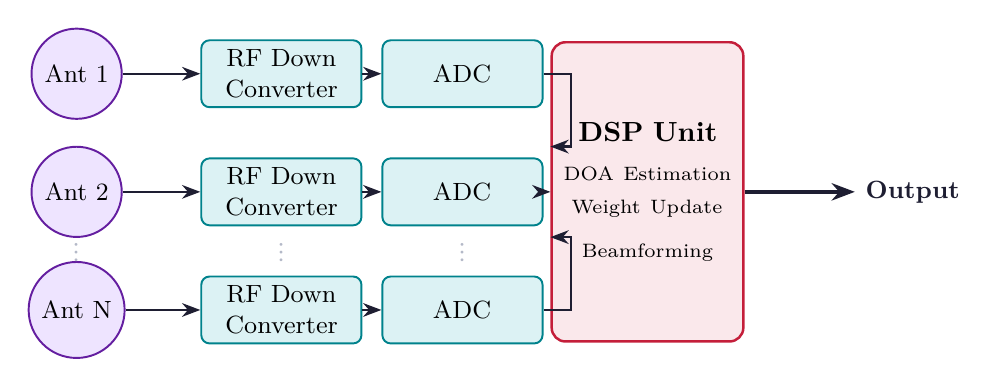
\begin{tikzpicture}[
  sblock/.style={rectangle, draw=myteal, fill=hdrteal, text width=1.8cm,
    align=center, minimum height=0.85cm, font=\small,
    rounded corners=3pt, line width=0.7pt},
  ablock/.style={circle, draw=mypurple, fill=hdrpurple,
    minimum size=0.72cm, font=\small, line width=0.7pt}]

  % ── Row y-coordinates: evenly spaced ─────────────────────────────────────
  % Row 1 (Ant 1) at y=1.5, Row 2 (Ant 2) at y=0, Row N at y=-1.5
  % Dot row midway between rows 2 and N at y=-0.75

  % ── Column x-coordinates ──────────────────────────────────────────────────
  % Ant: x=0, RF: x=2.4, ADC: x=4.65, DSP: x=7.0

  % ── Antenna column ────────────────────────────────────────────────────────
  \node[ablock] (a1) at (0,  1.5) {Ant 1};
  \node[ablock] (a2) at (0,  0.0) {Ant 2};
  \node[ablock] (aN) at (0, -1.5) {Ant N};

  % ── RF Downconverter column ───────────────────────────────────────────────
  \node[sblock] (rf1) at (2.6,  1.5) {RF Down\\Converter};
  \node[sblock] (rf2) at (2.6,  0.0) {RF Down\\Converter};
  \node[sblock] (rfN) at (2.6, -1.5) {RF Down\\Converter};

  % ── ADC column ────────────────────────────────────────────────────────────
  \node[sblock] (adc1) at (4.9,  1.5) {ADC};
  \node[sblock] (adc2) at (4.9,  0.0) {ADC};
  \node[sblock] (adcN) at (4.9, -1.5) {ADC};

  % ── DSP Unit — centred at y=0, height spans all 3 rows ────────────────────
  \node[draw=myred, fill=hdrred, line width=0.9pt, rounded corners=5pt,
        minimum height=3.8cm, text width=2.2cm, align=center]
       (dsp) at (7.25, 0)
       {\textbf{DSP Unit}\\[6pt]
        \scriptsize DOA Estimation\\[4pt]
        \scriptsize Weight Update\\[4pt]
        \scriptsize Beamforming};

  % ── Dot rows — centred in the gap between row 2 and row N ─────────────────
  \node[font=\normalsize, color=mgframe] at (0,   -0.77) {$\vdots$};
  \node[font=\normalsize, color=mgframe] at (2.6, -0.77) {$\vdots$};
  \node[font=\normalsize, color=mgframe] at (4.9, -0.77) {$\vdots$};

  % ── Connections — row 1 ───────────────────────────────────────────────────
  \draw[arrow] (a1)   -- (rf1);
  \draw[arrow] (rf1)  -- (adc1);
  \draw[arrow] (adc1.east) -- ++(0.35,0) |- (dsp.155);

  % ── Connections — row 2 ───────────────────────────────────────────────────
  \draw[arrow] (a2)   -- (rf2);
  \draw[arrow] (rf2)  -- (adc2);
  \draw[arrow] (adc2.east) -- (dsp.west);

  % ── Connections — row N ───────────────────────────────────────────────────
  \draw[arrow] (aN)   -- (rfN);
  \draw[arrow] (rfN)  -- (adcN);
  \draw[arrow] (adcN.east) -- ++(0.35,0) |- (dsp.205);

  % ── Output ────────────────────────────────────────────────────────────────
  \draw[arrow, line width=1.2pt] (dsp.east) -- ++(1.4,0)
    node[right, font=\small\bfseries\color{mydark}] {Output};

\end{tikzpicture}
\end{tcolorbox}

\subsection{Beamforming Basics}
\begin{itemize}[leftmargin=*, itemsep=3pt]
  \item \textbf{Phased Array / Fixed-Weight Beamforming:} The weights (amplitudes and phases) are predefined or adjusted using analog phase shifters to steer the main beam in a specific fixed direction.
  \item \textbf{Adaptive Beamforming:} The weights are dynamically computed in real-time by a DSP processor using feedback algorithms to optimize the Signal-to-Interference-plus-Noise Ratio (SINR).
  \item \textbf{Algorithms:} Common adaptive weight-updating algorithms include:
    \begin{itemize}[leftmargin=*, itemsep=1pt]
      \item \textbf{LMS (Least Mean Squares):} Low complexity, gradient descent.
      \item \textbf{RLS (Recursive Least Squares):} Fast convergence, high complexity.
      \item \textbf{MUSIC / ESPRIT:} High-resolution algorithms used to find the Direction of Arrival (DOA) of incoming signals.
    \end{itemize}
\end{itemize}

\subsection{Weight Vector Formulation}
Let the $N$-element array receive a signal. The received signal vector is:
\[
\mathbf{x}(t) = [x_1(t),\ x_2(t),\ \dots,\ x_N(t)]^T
\]
The array output is a linear combination of the received signals weighted by a complex weight vector $\mathbf{w} = [w_1, w_2, \dots, w_N]^T$:
\[
y(t) = \mathbf{w}^H \mathbf{x}(t) = \sum_{n=1}^{N} w_n^* x_n(t)
\]
where $(\cdot)^H$ denotes the Hermitian (conjugate transpose). The weights control both the amplitude and phase applied to each antenna element output.

\textbf{Fixed-weight (Conventional) Beamformer:} For steering toward direction $\theta_0$, the optimal weights are the \textbf{steering vector} $\mathbf{a}(\theta_0)$:
\[
\mathbf{w} = \mathbf{a}(\theta_0) = [1,\ e^{j\psi},\ e^{j2\psi},\ \dots,\ e^{j(N-1)\psi}]^T, \quad \psi = kd\cos\theta_0
\]
This applies a phase ramp across the array to align and coherently add the signals from direction $\theta_0$.

\subsection{LMS Adaptive Algorithm}
The \textbf{Least Mean Squares (LMS)} algorithm updates the weight vector iteratively to minimize the mean square error between the array output $y(k)$ and a reference signal $d(k)$ (desired signal):

\begin{tcolorbox}[formulabox, title={\textbf{LMS Weight Update Rule}}]
\[
e(k) = d(k) - \mathbf{w}^H(k)\,\mathbf{x}(k) \quad \text{(error signal)}
\]
\[
\mathbf{w}(k+1) = \mathbf{w}(k) + 2\mu\, \mathbf{x}(k)\, e^*(k) \quad \text{(weight update)}
\]
where $\mu$ is the step-size parameter ($0 < \mu < \frac{1}{N \cdot P_{in}}$, $P_{in}$ = input power).
\end{tcolorbox}

\begin{itemize}[leftmargin=*, itemsep=2pt]
  \item \textbf{Small $\mu$:} Slow convergence, low misadjustment (stable, accurate steady state).
  \item \textbf{Large $\mu$:} Fast convergence, high misadjustment (may diverge if too large).
  \item The LMS algorithm steers the main beam toward the desired user while automatically placing nulls in the directions of interferers — no explicit knowledge of interferer locations is needed.
\end{itemize}

\begin{tcolorbox}[tikzbox, title={Switched-Beam vs. Adaptive Array Patterns}]
\centering
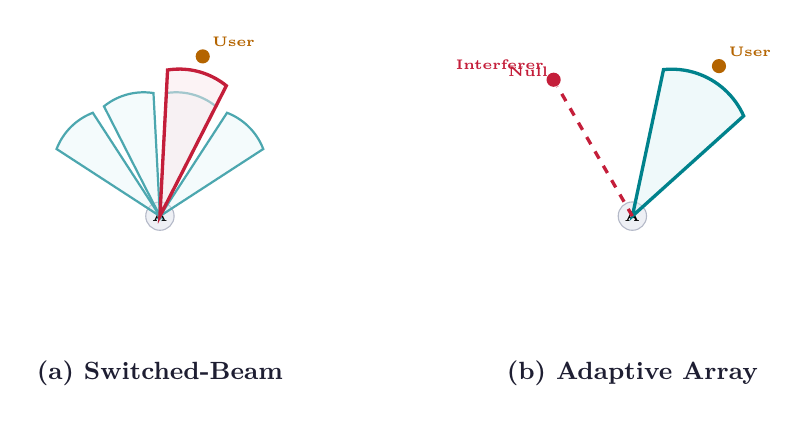
\begin{tikzpicture}[scale=1.0]
  % ── (a) Switched-Beam ──────────────────────────────────────────────────────
  \begin{scope}[xshift=-3.0cm]
    % Array element at centre
    \fill[hdrgray, draw=mgframe] (0,0) circle (0.18);
    \node[font=\tiny\bfseries] at (0,0) {A};

    % Four fixed beams as filled wedges (using proper polar coords)
    % Beam angles from vertical: 45, 75, 105, 135 deg (measured from positive x-axis)
    \foreach \ang/\hw in {45/12, 75/12, 105/12, 135/12} {
      \draw[color=myteal!70, fill=hdrteal, fill opacity=0.30, thick,
            domain={-\hw}:{\hw}, samples=20, variable=\r]
        plot ({1.6*cos(\r)*cos(\ang + \r)}, {1.6*cos(\r)*sin(\ang + \r)}) -- (0,0) -- cycle;
    }
    % Active (selected) beam highlighted in red — beam at 75 deg
    \draw[color=myred, fill=hdrred, fill opacity=0.5, very thick,
          domain=-12:12, samples=20, variable=\r]
      plot ({1.9*cos(\r)*cos(75 + \r)}, {1.9*cos(\r)*sin(75 + \r)}) -- (0,0) -- cycle;

    % User dot
    \fill[myamber] ({2.1*cos(75)},{2.1*sin(75)}) circle (0.09)
      node[above right, font=\tiny\bfseries\color{myamber}] {User};

    \node[font=\small\bfseries\color{mydark}] at (0,-2.0) {(a) Switched-Beam};
  \end{scope}

  % ── (b) Adaptive Array ─────────────────────────────────────────────────────
  \begin{scope}[xshift=3.0cm]
    % Array element
    \fill[hdrgray, draw=mgframe] (0,0) circle (0.18);
    \node[font=\tiny\bfseries] at (0,0) {A};

    % Steered beam toward user at 60 deg (narrow)
    \draw[color=myteal, fill=hdrteal, fill opacity=0.45, very thick,
          domain=-18:18, samples=25, variable=\r]
      plot ({2.0*cos(\r)*cos(60 + \r)}, {2.0*cos(\r)*sin(60 + \r)}) -- (0,0) -- cycle;

    % Null line toward interferer at 120 deg
    \draw[very thick, color=myred, dashed] (0,0) -- ({1.9*cos(120)},{1.9*sin(120)});
    \node[above left, font=\tiny\bfseries\color{myred}] at ({1.9*cos(120)},{1.9*sin(120)}) {Null};

    % User and interferer dots
    \fill[myamber] ({2.2*cos(60)},{2.2*sin(60)}) circle (0.09)
      node[above right, font=\tiny\bfseries\color{myamber}] {User};
    \fill[myred] ({2.0*cos(120)},{2.0*sin(120)}) circle (0.09)
      node[above left, font=\tiny\bfseries\color{myred}] {Interferer};

    \node[font=\small\bfseries\color{mydark}] at (0,-2.0) {(b) Adaptive Array};
  \end{scope}
\end{tikzpicture}
\end{tcolorbox}

% ===============================================================================
\section{Radio Wave Propagation Modes}
% ===============================================================================

Radio waves propagate from transmitter to receiver via three primary modes depending on their frequency.

\begin{tcolorbox}[tikzbox, title={Radio Wave Propagation Modes}]
\centering
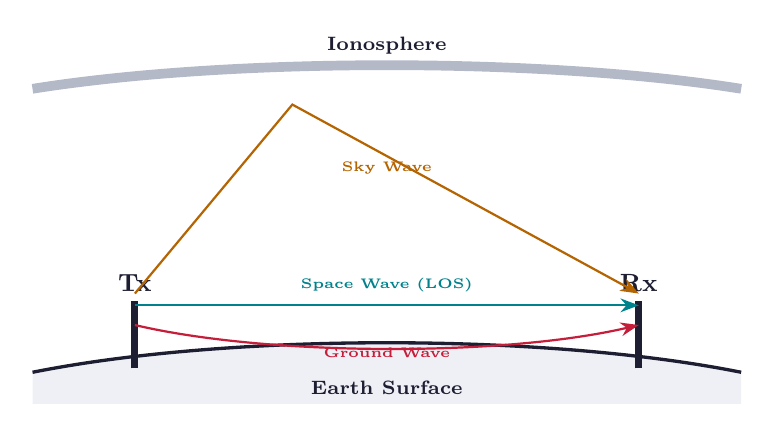
\begin{tikzpicture}[scale=1.0]
  % ── Earth surface (gentle arc, bounded) ────────────────────────────────────
  \fill[hdrgray] (-4.5,-1.4) .. controls (-2,-0.9) and (2,-0.9) .. (4.5,-1.4) --
                 (4.5,-1.8) -- (-4.5,-1.8) -- cycle;
  \draw[very thick, color=mydark] (-4.5,-1.4) .. controls (-2,-0.9) and (2,-0.9) .. (4.5,-1.4);
  \node[font=\scriptsize\bfseries\color{mydark}] at (0,-1.6) {Earth Surface};

  % ── Ionosphere (arc at top, bounded) ───────────────────────────────────────
  \draw[line width=3.5pt, color=mgframe]
    (-4.5, 2.2) .. controls (-2, 2.6) and (2, 2.6) .. (4.5, 2.2);
  \node[font=\scriptsize\bfseries\color{mydark}] at (0, 2.75) {Ionosphere};

  % ── Tx and Rx towers ───────────────────────────────────────────────────────
  \draw[line width=2.5pt, color=mydark] (-3.2,-1.35) -- (-3.2,-0.5);
  \node[above, font=\small\bfseries\color{mydark}] at (-3.2,-0.5) {Tx};

  \draw[line width=2.5pt, color=mydark] (3.2,-1.35) -- (3.2,-0.5);
  \node[above, font=\small\bfseries\color{mydark}] at (3.2,-0.5) {Rx};

  % ── 1. Ground Wave ─────────────────────────────────────────────────────────
  \draw[thick, color=myred, -Stealth]
    (-3.2,-0.8) .. controls (-1.5,-1.2) and (1.5,-1.2) .. (3.2,-0.8);
  \node[font=\tiny\bfseries\color{myred}] at (0,-1.15) {Ground Wave};

  % ── 2. Space Wave (LOS) ────────────────────────────────────────────────────
  \draw[thick, color=myteal, -Stealth] (-3.2,-0.55) -- (3.2,-0.55);
  \node[above, font=\tiny\bfseries\color{myteal}] at (0,-0.5) {Space Wave (LOS)};

  % ── 3. Sky Wave ────────────────────────────────────────────────────────────
  \draw[thick, color=myamber, -Stealth]
    (-3.2,-0.4) -- (-1.2, 2.0) -- (3.2,-0.4);
  \node[font=\tiny\bfseries\color{myamber}] at (0, 1.2) {Sky Wave};
\end{tikzpicture}
\end{tcolorbox}

\subsection{Ground Wave (Surface Wave) Propagation}
Ground waves travel along the surface of the Earth, guided by the boundary between the atmosphere and the ground.
\begin{itemize}[leftmargin=*, itemsep=2pt]
  \item \textbf{Frequency Range:} Very Low Frequency (VLF) to Medium Frequency (MF) ($< 2\,\text{MHz}$).
  \item \textbf{Mechanism:} The wave induces currents in the ground, causing attenuation. Attenuation increases rapidly with frequency, limiting this mode to low frequencies.
  \item \textbf{Application:} AM radio broadcasting, maritime communications.
\end{itemize}

\subsection{Space Wave (Line-of-Sight) Propagation}
Space waves travel through the troposphere directly from transmitter to receiver, or via ground reflection.
\begin{itemize}[leftmargin=*, itemsep=2pt]
  \item \textbf{Frequency Range:} Very High Frequency (VHF) and above ($> 30\,\text{MHz}$).
  \item \textbf{Radio Horizon ($d$):} The maximum line-of-sight distance is limited by the curvature of the Earth. Accounting for atmospheric refraction (effective Earth radius factor $k = 4/3$):
  \[
  d \approx \sqrt{17 h_t} + \sqrt{17 h_r} \approx 4.12 \left( \sqrt{h_t} + \sqrt{h_r} \right) \,\text{km}
  \]
  where $h_t$ and $h_r$ are the heights of the transmitting and receiving towers in meters.
  \item \textbf{Other modes:} Tropospheric scatter, duct propagation.
\end{itemize}

\subsection{Sky Wave Propagation}
Sky waves travel upward and are reflected (refracted) back to Earth by the ionosphere.
\begin{itemize}[leftmargin=*, itemsep=2pt]
  \item \textbf{Frequency Range:} High Frequency (HF) ($3$–$30\,\text{MHz}$).
  \item \textbf{Ionospheric Layers:} Formed by solar UV/X-ray ionization.
\end{itemize}

\par\noindent
\textbf{Ionosphere Layers Properties:}\par\noindent
{\renewcommand{\arraystretch}{1.45}%
\begin{tabularx}{\linewidth}{|B{1.5cm}|B{2.2cm}|Y|Y|}
\hline
\textbf{Layer} & \textbf{Altitude} & \textbf{Day Behavior} & \textbf{Night Behavior} \\
\hline
D Layer & $50$–$90\,\text{km}$ & Absorbs HF; reflects VLF/LF. & Disappears (recombines). \\
\hline
E Layer & $90$–$140\,\text{km}$ & Partially reflects HF. & Weakens significantly. \\
\hline
F1 Layer & $140$–$250\,\text{km}$ & Merges with F2 at night. & Disappears. \\
\hline
F2 Layer & $250$–$400\,\text{km}$ & Highest electron density; primary sky wave reflector. & Merges into a single F layer. \\
\hline
\end{tabularx}}

% ===============================================================================
\section{Ionospheric Parameters}
% ===============================================================================

The ionosphere acts as a refracting medium. Its refractive index $n$ is:
\[
n = \sqrt{1 - \frac{81 N}{f^2}}
\]
where $N$ is the electron density (electrons/$\text{m}^3$) and $f$ is the wave frequency (Hz).

\textbf{Physical Interpretation:} When a sky wave enters the ionosphere at an oblique angle, successive layers of increasing electron density bend the wave progressively away from vertical (like Snell's law in optics). Eventually, at the height where $n = \cos\theta_i$, the wave is totally reflected and returns to Earth. If the frequency is too high, $n$ never equals $\cos\theta_i$ and the wave escapes into space.

\subsection{Virtual Height}
The \textbf{virtual height} ($h_{virt}$) is the apparent height from which a short pulse of radio energy appears to be reflected, assuming the wave traveled at the speed of light in free space for the entire round trip. It is always greater than the actual reflection height because the wave slows down as electron density increases.
\[
h_{virt} = \frac{c \cdot \Delta t}{2}
\]
where $\Delta t$ is the round-trip time for a vertically launched pulse.

\subsection{Lowest Usable Frequency (LUF)}
The \textbf{LUF} is the lowest frequency at which sky-wave communication is possible over a given path. Below the LUF, the D-layer absorption becomes so severe that the signal is absorbed before reaching the receiver. The LUF depends on:
\begin{itemize}[leftmargin=*, itemsep=2pt]
  \item Solar activity (higher absorption during daytime and solar maxima).
  \item Path length and required signal level.
  \item Transmitter power (higher power lowers the effective LUF).
\end{itemize}
The \textbf{Optimum Working Frequency (OWF)} is typically chosen as $85\%$ of the MUF to provide a safety margin against day-to-day variability:
\[
f_{OWF} \approx 0.85 \times f_{MUF}
\]

\begin{tcolorbox}[formulabox, title={\textbf{Key Sky-Wave Design Parameters}}]
\begin{enumerate}[leftmargin=*, label=\textbf{\arabic*.}, itemsep=3pt, topsep=1pt]
  \item \textbf{Critical Frequency ($f_c$):} The highest frequency that is reflected back to Earth when launched vertically ($90^\circ$ elevation):
  \[
  f_c = 9\sqrt{N_{max}}
  \]
  where $N_{max}$ is the maximum electron density in the reflecting layer (electrons/m$^3$).
  \item \textbf{Maximum Usable Frequency (MUF):} The highest frequency reflected back to Earth when launched at an oblique angle of incidence $\theta_i$ (measured from vertical):
  \[
  f_{MUF} = f_c \sec\theta_i = \frac{f_c}{\cos\theta_i} \quad (\text{Secant Law})
  \]
  For a flat Earth approximation with path length $D$ and reflection height $h$:
  \[
  \sec\theta_i = \sqrt{1 + \left(\frac{D}{2h}\right)^{\!2}}
  \]
  \item \textbf{Skip Distance ($D_{skip}$):} The minimum distance from the transmitter where a sky wave of frequency $f$ ($f > f_c$) returns to Earth. Within this distance, no sky-wave signal is received — this region is called the \textbf{skip zone}:
  \[
  D_{skip} = 2 h_{virt} \sqrt{\left(\frac{f_{MUF}}{f_c}\right)^{\!2} - 1}
  \]
  \item \textbf{Optimum Working Frequency (OWF):}
  \[
  f_{OWF} \approx 0.85 \times f_{MUF}
  \]
\end{enumerate}
\end{tcolorbox}

\subsection{Skip Zone and Dead Zone}
\begin{itemize}[leftmargin=*, itemsep=3pt]
  \item \textbf{Skip Zone (Dead Zone):} The annular region around the transmitter where neither the ground wave (which has died out) nor the sky wave (which overshoots) can be received. For a sky wave of frequency $f$, the inner edge of the skip zone is at the skip distance $D_{skip}$.
  \item \textbf{Effect of Frequency:} As frequency increases toward the MUF, the skip distance increases. As frequency decreases toward $f_c$, the skip distance decreases to zero (the wave returns almost vertically).
  \item \textbf{Multiple Hops:} Sky waves can undergo successive reflections between the ionosphere and the Earth's surface, allowing communication over very long distances ($> 10{,}000\,\text{km}$).
\end{itemize}

% ===============================================================================
% MANDATORY QUICK REVISION PAGE
% ===============================================================================
\newpage
\begin{center}
  {\large\bfseries\color{myred} Quick Revision --- Module 7}\\[3pt]
  {\small\color{mydark} Smart Antennas and Propagation $|$ PE-EC801A}
\end{center}
\noindent{\color{myred}\rule{\linewidth}{1.2pt}}
\vspace{4pt}

\begin{tcolorbox}[formulabox, title={\textbf{Key Formulas and Metrics at a Glance}}]
\renewcommand{\arraystretch}{1.35}
\begin{tabularx}{\linewidth}{B{5.2cm} X}
Radio Horizon Distance ($d$) & $d \approx 4.12 (\sqrt{h_t} + \sqrt{h_r})$ \quad (in km, $h$ in meters) \\[4pt]
Ionospheric Refractive Index ($n$) & $n = \sqrt{1 - \frac{81 N}{f^2}}$ \\[4pt]
Critical Frequency ($f_c$) & $f_c = 9\sqrt{N_{max}}$ \quad (vertical incidence) \\[4pt]
Oblique Secant Law (MUF) & $f_{MUF} = f_c \sec\theta_i$ \\[4pt]
Skip Distance ($D_{skip}$) & $D_{skip} = 2 h \sqrt{(f_{MUF}/f_c)^2 - 1}$ \\[4pt]
Smart Weight Vector ($\vec{w}$) & $\vec{y}(t) = \vec{w}^H \vec{x}(t)$ \quad (combining array outputs) \\
\end{tabularx}
\end{tcolorbox}

\begin{tcolorbox}[defbox, title={\textbf{One-Line Definitions}}]
\begin{itemize}[leftmargin=*, itemsep=2pt, topsep=0pt]
  \item \textbf{DOA Estimation:} Direction of Arrival; calculating the angle from which a signal hits the antenna array.
  \item \textbf{Adaptive Beamforming:} Real-time DSP weight adjustment to maximize wanted signals and null out noise/interference.
  \item \textbf{Ground Wave:} A low-frequency electromagnetic wave that travels guided by the curvature and conductivity of the Earth.
  \item \textbf{Skip Distance:} The minimum distance from a transmitter where sky wave signals return to the Earth's surface.
  \item \textbf{Critical Frequency:} The limit frequency below which waves return to Earth at vertical incidence, and above which they escape to space.
  \item \textbf{Duct Propagation:} The trapping of VHF/UHF waves in a tropospheric layer due to temperature inversions, allowing long-range propagation.
\end{itemize}
\end{tcolorbox}

\begin{tcolorbox}[exambox, title={\textbf{Frequently Asked / Viva Questions}}]
\begin{enumerate}[topsep=0pt, label=\textbf{Q\arabic*.}, itemsep=5pt]
  \item \Q{What are the benefits of using smart antennas in wireless networks?}
    Smart antennas increase system capacity (via Space Division Multiple Access - SDMA), extend coverage range (via directive beam gain), reduce co-channel interference (by steering nulls toward interferers), and mitigate multipath fading.
  \item \Q{Compare switched-beam and adaptive array smart antennas.}
    Switched-beam systems select from a set of predefined, fixed beams. Adaptive arrays continuously track the user's location and steer the beam and nulls dynamically using DSP algorithms, offering higher performance but at a higher cost.
  \item \Q{Explain the physical mechanism of ground wave propagation. Why is it limited to low frequencies?}
    As ground waves travel, they induce currents in the Earth's surface. Since the Earth acts as a lossy dielectric, it dissipates power. Ground attenuation increases rapidly with frequency, limiting this mode to frequencies below $2\,\text{MHz}$.
  \item \Q{Define critical frequency, MUF, and skip zone.}
    \begin{itemize}[leftmargin=*, itemsep=1pt, topsep=2pt]
      \item \textbf{Critical Frequency ($f_c$):} The maximum frequency reflected at vertical incidence.
      \item \textbf{MUF:} The maximum frequency reflected at oblique incidence ($f_{MUF} = f_c \sec\theta_i$).
      \item \textbf{Skip Zone:} The region between the limit of ground-wave coverage and the point where the first sky-wave returns to Earth. No signal is received in this zone.
    \end{itemize}
  \item \Q{Why does the D-layer of the ionosphere disappear at night?}
    The D-layer is the lowest layer ($50$–$90\,\text{km}$) where atmospheric density is high. It is ionized during the day by solar radiation. At night, without solar rays, free electrons recombine rapidly with ions due to the high collision rate, causing the layer to disappear.
  \item \Q{State the formula for the line-of-sight range of space waves. How does the earth's atmosphere affect it?}
    $d \approx 4.12 (\sqrt{h_t} + \sqrt{h_r})$ km. The atmosphere has a refractive index that decreases with height, which bends waves slightly downward, extending the radio horizon about $15\%$ beyond the geometric optical horizon. This is modeled using an effective Earth radius factor $k = 4/3$.
\end{enumerate}
\end{tcolorbox}

\begin{tcolorbox}[tikzbox, title={Comparison of Wave Propagation Modes}]
\centering
\renewcommand{\arraystretch}{1.55}
{\renewcommand{\arraystretch}{1.55}%
\begin{tabularx}{\linewidth}{|B{3.2cm}|Y|Y|Y|}
\hline
\multicolumn{1}{|>{\centering\arraybackslash}m{3.2cm}|}{\textbf{Parameter}} &
\multicolumn{1}{>{\centering\arraybackslash}Y|}{\textbf{Ground Wave}} &
\multicolumn{1}{>{\centering\arraybackslash}Y|}{\textbf{Space Wave}} &
\multicolumn{1}{>{\centering\arraybackslash}Y|}{\textbf{Sky Wave}} \\
\hline
Frequency Range & $< 2\,\text{MHz}$ (LF/MF) & $> 30\,\text{MHz}$ (VHF/UHF/SHF) & $3$–$30\,\text{MHz}$ (HF) \\
\hline
Propagation Path & Curves along Earth's surface & Direct line-of-sight path & Ionospheric reflection/refraction \\
\hline
Primary Limitation & High ground attenuation at higher frequencies & Earth curvature blockage (radio horizon) & Solar ionization variations (day/night/seasonal) \\
\hline
Typical Applications & AM radio, maritime navigation & FM, TV, cellular, satellite & Long-range amateur radio, SW broadcasting \\
\hline
\end{tabularx}}
\end{tcolorbox}


\end{document}
